\clearpage
\chapter{HNL discovery with the DUNE experiment}
\label{cha:hnl_dune}

It is exciting to note that current and upcoming neutrino oscillation
experiments will be able to perform beam dump style measurements \cite{Kusenko:2004qc, Asaka:2012bb, Abe:2019kgx}. 
%
A crucial difference between oscillation detectors and dedicated beam dump searches of the past is that %
the former tries to maximise its Standard Model neutrino scattering rate, while the latter goes to lengths %
to suppress it in order to reduce backgrounds.
%
However, for some of the current and future accelerator neutrino experiments, %
such as the Short Baseline Neutrino (SBN) program~\cite{Antonello:2015lea}, %
the strong particle reconstruction capabilities of Liquid Argon detectors and distinctive kinematics %
of neutrino decays have been shown to allow competitive bounds on heavy neutrinos %
to be made despite naively large backgrounds \cite{Ballett:2016opr}. 
%
Long baseline oscillation experiments, such as the upcoming Deep Underground Neutrino Experiment (DUNE)~\cite{Abi:2018dnh}, %
will see a greatly diluted flux of nearly-sterile neutrinos at their far detectors and consequently poor sensitivity.
However, the DUNE Near Detector (DUNE ND), placed \np{574}\,m from the target, has a great potential %
for searches for new physics~\cite{Adams:2013qkq}.
Even if the final design of the ND has not been confirmed as yet, the options being considered combine a large active volume, %
in close proximity to a very intense neutrino beam and cutting-edge event reconstruction capabilities.
These will allow DUNE ND to undertake valuable searches for BSM physics in a entirely complementary way %
to the central oscillation physics programme. 

The strongest limits were set by the PS191 experiment~\cite{Bernardi:1985ny, Bernardi:1987ek}, %
a beam dump experiment which ran at CERN in 1984.

In this chapter, we present a detailed analysis of the sensitivity of DUNE ND to HNL in beam dump style searches.
We ground our discussion in theoretically consistent models, in which sterile neutrinos %
are associated with neutrino mass generation via a low-scale seesaw mechanism.
We extend and refine previous analysis~\cite{Krasnov:2019kdc, Adams:2013qkq}, %
using the latest configuration of the DUNE ND~\cite{DUNETDR:2019, DUNEND:2019}.
%Differently from previous sensitivity studies
%we ground our discussion in theoretically consistent models, in which sterile neutrinos are associated with neutrino %
%mass generation via a low-scale seesaw mechanism. %, such as inverse seesaw (ISS) mechanisms.
We note that the range of masses and mixing angles testable at DUNE~ND is of interest for the generation of %
the baryon asymmetry in the context of the ASR mechanism~\cite{Akhmedov:1998qx, Asaka:2005pn, Hernandez:2015wna, Hernandez:2016kel, Drewes:2017zyw}.
We consider both Majorana and pseudo-Dirac states and calculate their decay and production rates, 
with careful consideration given to helicity arguments.
These formulae are then used to estimate the sensitivity of the experiment, %
taking into account the beam and detector performance capabilities thanks to simulations of both event and background signals.
We stress that DUNE will be able to extend the current limits on new fermionic singlets, %
including those with masses above 500\,MeV, probing models of theoretical significance for the generation of neutrino mass.
We show that bounds can be put also on the mixing with tau neutrinos, thanks to the high energy~beam.

\section{The Near Detector of DUNE as a beam dump experiment}
\label{sec:beamdump}

\section{Simulation of events at DUNE ND}
\label{sec:experiment}

DUNE~\cite{Abi:2018dnh} is a long-baseline oscillation experiment that will study neutrino physics in great detail, %
focusing mainly on the determination of the CP violating phase, $\delta_\text{CP}$, %
of the mass ordering, %
%i.e.\ the sign of $\Delta m_{31}^2$,
and on the precision measurement of other oscillation parameters, in particular $\theta_{23}$.
These goals can be achieved thanks to both an intense neutrino beam and a high-resolution Far Detector (FD), %
consisting of a 40\,kt Liquid Argon Time Projection Chamber (LArTPC), situated \np{1300}\,km from the beam target.
The drift velocity of ionised electrons in LAr, typically of the order of cm/\textmu s, %
can be controlled with sufficient precision, by tuning the electric field, %
to result in high spatial resolution for event reconstruction~\cite{Rubbia:1977zz}.
%The c
%with liquefied argon instead of its gaseous phase.
%The LAr is advantageous compared to the gaseous counterpart because it is around one thousand times denser, %
%increasing the interaction probability, which is valuable for neutrino physics.
%Employing very pure argon, the recombination of released electrons can be reduced and %
%so the LArTPC design can be scaled to large volumes, as it will be done for DUNE.
%LAr also scintillates with a high light yield, around 40 photons/keV, but, differently from other liquefied noble gasses, %
%LAr is transparent to its scintillation wavelength, which peaks at \np{126.8}~nm.
%A photo-detection system can collect the scintillation light giving an additional handle on event reconstruction.
%All these exceptional properties make LArTPC a powerful tool for precision neutrino physics.
A very sensitive FD alone, however, is not enough due to numerous uncertainties on neutrino flux and cross sections.
A smaller and closer detector, called Near Detector (ND), is therefore adopted to normalise the flux of neutrinos reaching the FD and to help cancel out many of %
the neutrino-nucleon cross section systematics.

The DUNE ND will be placed \np{574}\,m from the target.
Its definitive design has not been finalised yet, but it will likely be a hybrid concept, %
consisting of a small LArTPC placed in front of a magnetised high-pressure gaseous TPC~\cite{DUNETDR:2019, DUNEND:2019}.
This module is complementary to the front detector, controlling escaping or below-threshold particles from the LArTPC, %
but is also capable of performing standalone measurement.
For its versatile nature, it is called Multi-Purpose Detector (MPD).
The sub-system LArTPC/MPD will be movable inside the ND hall---following the DUNE-PRISM concept---for %
better profiling the neutrino flux at different angles.
There will be a third module, a 3D Scintillation Tracker (3DST), on-axis, to monitor %
the stability of the beam flux and neutron contamination.
Currently, the proposed fiducial volume for the LArTPC module is 36\,m\tapi{3} and 50\,t of LAr, %
employing the ArgonCube technology~\cite{Amsler:1993255}, %
whereas the design for the MPD is based on the TPC in \mbox{ALICE}~\cite{Glassel:2004jv}, %
a cylinder of 102\,m\tapi{3} with gas at a pressure of 10\,atm and a fiducial mass of~1\,t.
The gas assumed for the studies in the TDR is a an 80--20 mixture of Ar--CH\tped{4}.
The~3DST is designed to have a fiducial mass of around \np{8.7}\,t of plastic scintillating material and %
wavelength shifting plates.
%($3\times2\times6$)\,m\tapi{3},
%and for the HPArFGT is ($3.5\times3.5\times6.4$)\,m\tapi{3}.
For this analysis, we take only in account the two core sub-detectors, the LArTPC and the MPD.
The main difference between these two ND modules is that the gaseous TPC has a larger volume than the LArTPC.
This feature is favourable when studying rare events, like heavy neutrino decays, because more neutrinos enter the fiducial volume.
Furthermore, the lower density of the MPD helps reduce the number of neutrino scattering events, which are background to rare signatures.
Apart from volume and density differences and relative positions in the detector hall, %
we treat the two ND units as with similar detection performances, on-axis, and do not take in account the magnetisation of the gaseous~TPC. 
%Optical partitioning, short electron drift distance, and pixelated readout are features being taken in consideration to %
%improve the performance of the LArTPC to the anticipated high-rate environment %
%and the efficiency of reconstructing events at the near site.

Thanks to its proximity to the accelerator, the ND will be exposed to an extremely intense neutrino beam, %
with a flux peak around five million times greater than at the FD.
The Long Baseline Neutrino Facility (LBNF) at Fermilab will deploy a very energetic beam of protons, %
extracted from the Main Injector (MI) and delivered to a graphite target.
The collision produces secondary particles, which are collimated by a focusing horn system and then decay forming a neutrino beam.
Assuming an 80\,GeV proton beam at 1.2\,MW for the first six years and at 2.4\,MW for a second set of six years~\cite{Abi:2018dnh}, 
the ND will collect a total of \np{2.65e22} protons on target (POT) over the lifespan of the experiment, %
running for the same amount of time in neutrino and antineutrino mode.
The ND will be placed on-axis for half of the total runtime, whereas it will be positioned %
at different angles off-axis for the remaining acquisition period, enacting the DUNE-PRISM concept.
The search for HNL decays can benefit to some extent at off-axis angles, %
as the SM neutrino background is particularly reduced, despite a reduced event rate.
However, the modelling of the neutrino beam profile at different angles using only the on-axis spectrum is not trivial.
Half of the total statistics will be collected with a reversed horn current configuration, %
but the parentage composition of the neutrino spectrum with the antineutrino-mode beam is not available to us, %
as well as the off-axis beam flux.
In this work, we simply consider the on-axis configuration of the ND with a forward horn current configuration, %
which would correspond to a quarter of the runtime, or \np{0.66e22}\,POT.
The same analysis of this study can nonetheless be applied equally to the beam in antineutrino mode, %
which should result in a sensitivity similar to the neutrino mode configuration, %
being wary of the different composition of the neutrino spectrum.
Even though we cannot achieve an accurate estimate of the DUNE ND sensitivity, %
we make the naive assumption, with the above caveats, that the total sensitivity to HNL%
---including off-axis angles and antineutrino mode beam---%
is equivalent to six years of data taking, \ie \np{1.32e22}\,POT, %
with the beam in neutrino mode and the ND on-axis.

%In this work we consider only the beam in the neutrino mode configuration, %
%which corresponds to half of the total runtime, or \np{1.32e22}\,POT.
%The same study of this article can be applied equally to the beam in reversed horn current configuration, %
%but its details are not available to us.
%Including the analysis for the beam in antineutrino mode should result in an increment on the overall sensitivity, %
%approximately a factor of two better.

%Moreover, the ND system could implement the $\nu$PRISM concept~\cite{Bhadra:2014oma}, which would make the detector %
%	movable, to take advantage of the monochromatic nature of the neutrino beam off-axis.

\begin{table}
	\centering
	\small
	\begin{tabular}{lccccc}
		\toprule
		&\textbf{PS191}	& \textbf{DUNE ND}& \textbf{SBND}	& \textbf{NA62} & \textbf{SHiP} \\
		\midrule
		Baseline& 128\,m		    & 574\,m			& 110\,m		    & 220\,m         & 60\,m          \\
		Volume  & 216\,m\tapi{3} & 150\,m\tapi{3} & 80\,m\tapi{3}  & 750\,m\tapi{3} & 590\,m\tapi{3} \\
		Energy	& 19.2\,GeV	    & 80\,GeV	    & 8\,GeV		    & 400\,GeV       & 400\,GeV       \\
		POT	    & \np{0.86e19}	& \np{1.32e22}	& \np{6.6e20}	& \np{3e18}     & \np{2e20}     \\
		\midrule
		Exposure& 1.0 	        & 220.9         & 16.4	        & 8.5           & 5820          \\
		\bottomrule
	\end{tabular}
	\caption{Comparison between experiments mentioned in this work.
		The exposure is defined as POT$\times$Energy$\times$Volume$\times$Baseline${}^{-2}$ with respect to %
		PS191, where ``Energy'' is the proton beam energy.
		The NA62 and SHiP experiments are not directly comparable with SBND and DUNE ND, %
		in that different technologies are involved;
		the RICH detectors are adopted as fiducial volume for NA62, whereas %
		for SHiP, we estimate the volume as the cone contained in the ``hidden sector'' vacuum vessel. 
		The volume is a driving feature in the definition of the total exposure and it is of utter importance %
		for searches of decay-in-flight events.}
	\label{tab:nd}
\end{table}

A summary of the features of the ND system is reported in~\reftab{tab:nd}, where it is compared to other beam dump experiments: %
PS191~\cite{Bernardi:1985ny,Bernardi:1987ek}, SBND which is the detector of the SBN programme with the best sensitivity to %
HNL~\cite{Ballett:2016opr}, NA62~\cite{NA62:2017rwk}, and SHiP~\cite{Anelli:2015pba}.
We define the total exposure of the experiment as the proton accelerator beam power, integrated over the total run time, %
and scaled by the volume of the detector over its baseline squared.
The beam power times the run time corresponds to the number of POT times the proton energy. 
With this definition, an exposure twelve times bigger is expected for the DUNE ND system with respect to SBND, %
and around two hundred times bigger than PS191.
The NA62 and SHiP experiments have a different design and are not directly comparable to TPC and tracker experiments, %
but we report them here for thoroughness.
The estimated exposure of NA62 is limited by its number of POT and by just one year of data taking; %
despite this fact, the experiment is optimised to study kaon decays and has good %
sensitivity to HNL~\cite{Drewes:2018irr}.
The SHiP experiment presents an exposure thirty times bigger than DUNE ND, but the detector is specifically %
designed to search for BSM physics, including heavy neutrinos~\cite{SHiP:2018xqw} (see also~\refref{Caputo:2016ojx}).
The decay-in-flight search hugely benefits from its 50\,m long decay vessel and short baseline.

On the collider physics frontier, the MATHUSLA~\cite{Curtin:2018mvb} and the FASER~\cite{Ariga:2018uku} experiments %
will perform a dedicated search for extremely weakly-interacting and long lived particles, %
like HNLs for which they presents interesting sensitivity~\cite{Curtin:2018mvb, Kling:2018wct}.
MATHUSLA will be a \np{800e3}\,m\tapi{3} hodoscope placed on the surface above the ATLAS or the CMS detectors.
FASER will consist of a 10\,m cylindrical decay volume located 480\,m downstream of the ATLAS interaction point. 

\subsection{Flux prediction}
\label{sec:tauneutrino}

\begin{figure}
	\centering
	\resizebox{.5\textwidth}{!}{% GNUPLOT: LaTeX picture with Postscript
\begingroup
  \makeatletter
  \providecommand\color[2][]{%
    \GenericError{(gnuplot) \space\space\space\@spaces}{%
      Package color not loaded in conjunction with
      terminal option `colourtext'%
    }{See the gnuplot documentation for explanation.%
    }{Either use 'blacktext' in gnuplot or load the package
      color.sty in LaTeX.}%
    \renewcommand\color[2][]{}%
  }%
  \providecommand\includegraphics[2][]{%
    \GenericError{(gnuplot) \space\space\space\@spaces}{%
      Package graphicx or graphics not loaded%
    }{See the gnuplot documentation for explanation.%
    }{The gnuplot epslatex terminal needs graphicx.sty or graphics.sty.}%
    \renewcommand\includegraphics[2][]{}%
  }%
  \providecommand\rotatebox[2]{#2}%
  \@ifundefined{ifGPcolor}{%
    \newif\ifGPcolor
    \GPcolortrue
  }{}%
  \@ifundefined{ifGPblacktext}{%
    \newif\ifGPblacktext
    \GPblacktexttrue
  }{}%
  % define a \g@addto@macro without @ in the name:
  \let\gplgaddtomacro\g@addto@macro
  % define empty templates for all commands taking text:
  \gdef\gplbacktext{}%
  \gdef\gplfronttext{}%
  \makeatother
  \ifGPblacktext
    % no textcolor at all
    \def\colorrgb#1{}%
    \def\colorgray#1{}%
  \else
    % gray or color?
    \ifGPcolor
      \def\colorrgb#1{\color[rgb]{#1}}%
      \def\colorgray#1{\color[gray]{#1}}%
      \expandafter\def\csname LTw\endcsname{\color{white}}%
      \expandafter\def\csname LTb\endcsname{\color{black}}%
      \expandafter\def\csname LTa\endcsname{\color{black}}%
      \expandafter\def\csname LT0\endcsname{\color[rgb]{1,0,0}}%
      \expandafter\def\csname LT1\endcsname{\color[rgb]{0,1,0}}%
      \expandafter\def\csname LT2\endcsname{\color[rgb]{0,0,1}}%
      \expandafter\def\csname LT3\endcsname{\color[rgb]{1,0,1}}%
      \expandafter\def\csname LT4\endcsname{\color[rgb]{0,1,1}}%
      \expandafter\def\csname LT5\endcsname{\color[rgb]{1,1,0}}%
      \expandafter\def\csname LT6\endcsname{\color[rgb]{0,0,0}}%
      \expandafter\def\csname LT7\endcsname{\color[rgb]{1,0.3,0}}%
      \expandafter\def\csname LT8\endcsname{\color[rgb]{0.5,0.5,0.5}}%
    \else
      % gray
      \def\colorrgb#1{\color{black}}%
      \def\colorgray#1{\color[gray]{#1}}%
      \expandafter\def\csname LTw\endcsname{\color{white}}%
      \expandafter\def\csname LTb\endcsname{\color{black}}%
      \expandafter\def\csname LTa\endcsname{\color{black}}%
      \expandafter\def\csname LT0\endcsname{\color{black}}%
      \expandafter\def\csname LT1\endcsname{\color{black}}%
      \expandafter\def\csname LT2\endcsname{\color{black}}%
      \expandafter\def\csname LT3\endcsname{\color{black}}%
      \expandafter\def\csname LT4\endcsname{\color{black}}%
      \expandafter\def\csname LT5\endcsname{\color{black}}%
      \expandafter\def\csname LT6\endcsname{\color{black}}%
      \expandafter\def\csname LT7\endcsname{\color{black}}%
      \expandafter\def\csname LT8\endcsname{\color{black}}%
    \fi
  \fi
    \setlength{\unitlength}{0.0500bp}%
    \ifx\gptboxheight\undefined%
      \newlength{\gptboxheight}%
      \newlength{\gptboxwidth}%
      \newsavebox{\gptboxtext}%
    \fi%
    \setlength{\fboxrule}{0.5pt}%
    \setlength{\fboxsep}{1pt}%
\begin{picture}(7200.00,5040.00)%
    \gplgaddtomacro\gplbacktext{%
      \csname LTb\endcsname%%
      \put(924,704){\makebox(0,0)[r]{\strut{}\np{e8}}}%
      \put(924,2285){\makebox(0,0)[r]{\strut{}\np{e9}}}%
      \put(924,3867){\makebox(0,0)[r]{\strut{}\np{e10}}}%
      \put(1056,484){\makebox(0,0){\strut{}0}}%
      \put(2526,484){\makebox(0,0){\strut{}5}}%
      \put(3996,484){\makebox(0,0){\strut{}10}}%
      \put(5465,484){\makebox(0,0){\strut{}15}}%
      \put(6935,484){\makebox(0,0){\strut{}20}}%
    }%
    \gplgaddtomacro\gplfronttext{%
      \csname LTb\endcsname%%
      \put(176,2761){\rotatebox{-270}{\makebox(0,0){\strut{}$\nu_e / \text{cm}^2 / \text{GeV}$}}}%
      \put(3995,154){\makebox(0,0){\strut{}Energy (GeV)}}%
      \csname LTb\endcsname%%
      \put(6318,4624){\makebox(0,0)[r]{\strut{}Total}}%
      \csname LTb\endcsname%%
      \put(6318,4360){\makebox(0,0)[r]{\strut{}$\pi$}}%
      \csname LTb\endcsname%%
      \put(6318,4096){\makebox(0,0)[r]{\strut{}$K$}}%
      \csname LTb\endcsname%%
      \put(6318,3832){\makebox(0,0)[r]{\strut{}$K^0$}}%
      \csname LTb\endcsname%%
      \put(6318,3568){\makebox(0,0)[r]{\strut{}$\mu$}}%
      \csname LTb\endcsname%%
      \put(6318,3304){\makebox(0,0)[r]{\strut{}$D_s$}}%
    }%
    \gplbacktext
    \put(0,0){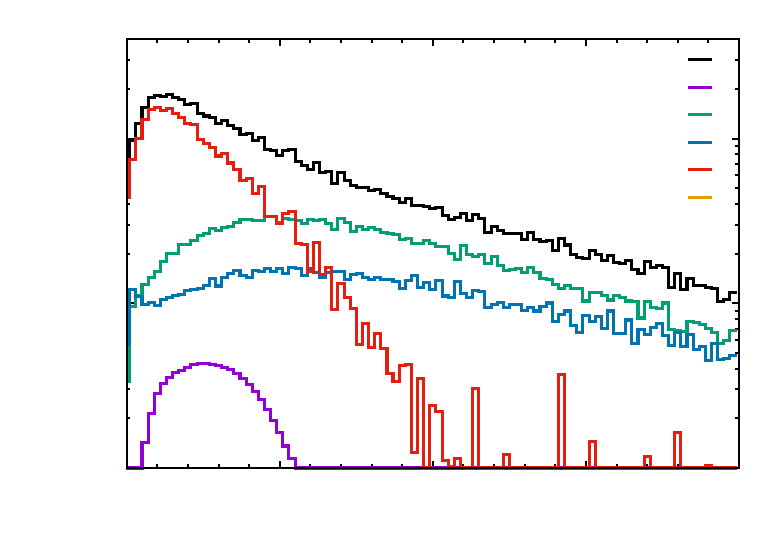
\includegraphics{pics/fluxnue}}%
    \gplfronttext
  \end{picture}%
\endgroup
}
	\hspace{-1em}
	\resizebox{.5\textwidth}{!}{% GNUPLOT: LaTeX picture with Postscript
\begingroup
  \makeatletter
  \providecommand\color[2][]{%
    \GenericError{(gnuplot) \space\space\space\@spaces}{%
      Package color not loaded in conjunction with
      terminal option `colourtext'%
    }{See the gnuplot documentation for explanation.%
    }{Either use 'blacktext' in gnuplot or load the package
      color.sty in LaTeX.}%
    \renewcommand\color[2][]{}%
  }%
  \providecommand\includegraphics[2][]{%
    \GenericError{(gnuplot) \space\space\space\@spaces}{%
      Package graphicx or graphics not loaded%
    }{See the gnuplot documentation for explanation.%
    }{The gnuplot epslatex terminal needs graphicx.sty or graphics.sty.}%
    \renewcommand\includegraphics[2][]{}%
  }%
  \providecommand\rotatebox[2]{#2}%
  \@ifundefined{ifGPcolor}{%
    \newif\ifGPcolor
    \GPcolortrue
  }{}%
  \@ifundefined{ifGPblacktext}{%
    \newif\ifGPblacktext
    \GPblacktexttrue
  }{}%
  % define a \g@addto@macro without @ in the name:
  \let\gplgaddtomacro\g@addto@macro
  % define empty templates for all commands taking text:
  \gdef\gplbacktext{}%
  \gdef\gplfronttext{}%
  \makeatother
  \ifGPblacktext
    % no textcolor at all
    \def\colorrgb#1{}%
    \def\colorgray#1{}%
  \else
    % gray or color?
    \ifGPcolor
      \def\colorrgb#1{\color[rgb]{#1}}%
      \def\colorgray#1{\color[gray]{#1}}%
      \expandafter\def\csname LTw\endcsname{\color{white}}%
      \expandafter\def\csname LTb\endcsname{\color{black}}%
      \expandafter\def\csname LTa\endcsname{\color{black}}%
      \expandafter\def\csname LT0\endcsname{\color[rgb]{1,0,0}}%
      \expandafter\def\csname LT1\endcsname{\color[rgb]{0,1,0}}%
      \expandafter\def\csname LT2\endcsname{\color[rgb]{0,0,1}}%
      \expandafter\def\csname LT3\endcsname{\color[rgb]{1,0,1}}%
      \expandafter\def\csname LT4\endcsname{\color[rgb]{0,1,1}}%
      \expandafter\def\csname LT5\endcsname{\color[rgb]{1,1,0}}%
      \expandafter\def\csname LT6\endcsname{\color[rgb]{0,0,0}}%
      \expandafter\def\csname LT7\endcsname{\color[rgb]{1,0.3,0}}%
      \expandafter\def\csname LT8\endcsname{\color[rgb]{0.5,0.5,0.5}}%
    \else
      % gray
      \def\colorrgb#1{\color{black}}%
      \def\colorgray#1{\color[gray]{#1}}%
      \expandafter\def\csname LTw\endcsname{\color{white}}%
      \expandafter\def\csname LTb\endcsname{\color{black}}%
      \expandafter\def\csname LTa\endcsname{\color{black}}%
      \expandafter\def\csname LT0\endcsname{\color{black}}%
      \expandafter\def\csname LT1\endcsname{\color{black}}%
      \expandafter\def\csname LT2\endcsname{\color{black}}%
      \expandafter\def\csname LT3\endcsname{\color{black}}%
      \expandafter\def\csname LT4\endcsname{\color{black}}%
      \expandafter\def\csname LT5\endcsname{\color{black}}%
      \expandafter\def\csname LT6\endcsname{\color{black}}%
      \expandafter\def\csname LT7\endcsname{\color{black}}%
      \expandafter\def\csname LT8\endcsname{\color{black}}%
    \fi
  \fi
    \setlength{\unitlength}{0.0500bp}%
    \ifx\gptboxheight\undefined%
      \newlength{\gptboxheight}%
      \newlength{\gptboxwidth}%
      \newsavebox{\gptboxtext}%
    \fi%
    \setlength{\fboxrule}{0.5pt}%
    \setlength{\fboxsep}{1pt}%
\begin{picture}(7200.00,5040.00)%
    \gplgaddtomacro\gplbacktext{%
      \csname LTb\endcsname%%
      \put(924,704){\makebox(0,0)[r]{\strut{}\np{e8}}}%
      \put(924,1527){\makebox(0,0)[r]{\strut{}\np{e9}}}%
      \put(924,2350){\makebox(0,0)[r]{\strut{}\np{e10}}}%
      \put(924,3173){\makebox(0,0)[r]{\strut{}\np{e11}}}%
      \put(924,3996){\makebox(0,0)[r]{\strut{}\np{e12}}}%
      \put(924,4819){\makebox(0,0)[r]{\strut{}\np{e13}}}%
      \put(1056,484){\makebox(0,0){\strut{}0}}%
      \put(2526,484){\makebox(0,0){\strut{}5}}%
      \put(3996,484){\makebox(0,0){\strut{}10}}%
      \put(5465,484){\makebox(0,0){\strut{}15}}%
      \put(6935,484){\makebox(0,0){\strut{}20}}%
    }%
    \gplgaddtomacro\gplfronttext{%
      \csname LTb\endcsname%%
      \put(176,2761){\rotatebox{-270}{\makebox(0,0){\strut{}$\nu_\mu / \text{cm}^2 / \text{GeV}$}}}%
      \put(3995,154){\makebox(0,0){\strut{}Energy (GeV)}}%
      \csname LTb\endcsname%%
      \put(6318,4624){\makebox(0,0)[r]{\strut{}Total}}%
      \csname LTb\endcsname%%
      \put(6318,4360){\makebox(0,0)[r]{\strut{}$\pi$}}%
      \csname LTb\endcsname%%
      \put(6318,4096){\makebox(0,0)[r]{\strut{}$K$}}%
      \csname LTb\endcsname%%
      \put(6318,3832){\makebox(0,0)[r]{\strut{}$K^0$}}%
      \csname LTb\endcsname%%
      \put(6318,3568){\makebox(0,0)[r]{\strut{}$\mu$}}%
      \csname LTb\endcsname%%
      \put(6318,3304){\makebox(0,0)[r]{\strut{}$D_s$}}%
    }%
    \gplbacktext
    \put(0,0){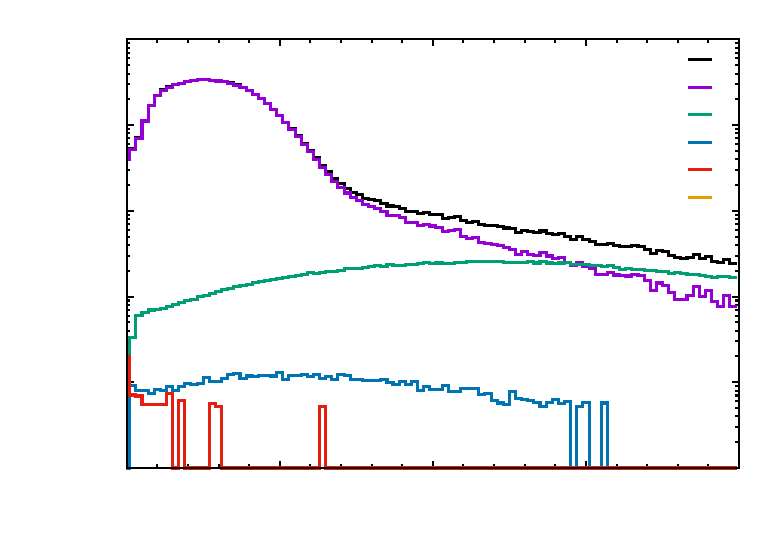
\includegraphics{pics/fluxnumu}}%
    \gplfronttext
  \end{picture}%
\endgroup
}
	\\
	\resizebox{.5\textwidth}{!}{% GNUPLOT: LaTeX picture with Postscript
\begingroup
  \makeatletter
  \providecommand\color[2][]{%
    \GenericError{(gnuplot) \space\space\space\@spaces}{%
      Package color not loaded in conjunction with
      terminal option `colourtext'%
    }{See the gnuplot documentation for explanation.%
    }{Either use 'blacktext' in gnuplot or load the package
      color.sty in LaTeX.}%
    \renewcommand\color[2][]{}%
  }%
  \providecommand\includegraphics[2][]{%
    \GenericError{(gnuplot) \space\space\space\@spaces}{%
      Package graphicx or graphics not loaded%
    }{See the gnuplot documentation for explanation.%
    }{The gnuplot epslatex terminal needs graphicx.sty or graphics.sty.}%
    \renewcommand\includegraphics[2][]{}%
  }%
  \providecommand\rotatebox[2]{#2}%
  \@ifundefined{ifGPcolor}{%
    \newif\ifGPcolor
    \GPcolortrue
  }{}%
  \@ifundefined{ifGPblacktext}{%
    \newif\ifGPblacktext
    \GPblacktexttrue
  }{}%
  % define a \g@addto@macro without @ in the name:
  \let\gplgaddtomacro\g@addto@macro
  % define empty templates for all commands taking text:
  \gdef\gplbacktext{}%
  \gdef\gplfronttext{}%
  \makeatother
  \ifGPblacktext
    % no textcolor at all
    \def\colorrgb#1{}%
    \def\colorgray#1{}%
  \else
    % gray or color?
    \ifGPcolor
      \def\colorrgb#1{\color[rgb]{#1}}%
      \def\colorgray#1{\color[gray]{#1}}%
      \expandafter\def\csname LTw\endcsname{\color{white}}%
      \expandafter\def\csname LTb\endcsname{\color{black}}%
      \expandafter\def\csname LTa\endcsname{\color{black}}%
      \expandafter\def\csname LT0\endcsname{\color[rgb]{1,0,0}}%
      \expandafter\def\csname LT1\endcsname{\color[rgb]{0,1,0}}%
      \expandafter\def\csname LT2\endcsname{\color[rgb]{0,0,1}}%
      \expandafter\def\csname LT3\endcsname{\color[rgb]{1,0,1}}%
      \expandafter\def\csname LT4\endcsname{\color[rgb]{0,1,1}}%
      \expandafter\def\csname LT5\endcsname{\color[rgb]{1,1,0}}%
      \expandafter\def\csname LT6\endcsname{\color[rgb]{0,0,0}}%
      \expandafter\def\csname LT7\endcsname{\color[rgb]{1,0.3,0}}%
      \expandafter\def\csname LT8\endcsname{\color[rgb]{0.5,0.5,0.5}}%
    \else
      % gray
      \def\colorrgb#1{\color{black}}%
      \def\colorgray#1{\color[gray]{#1}}%
      \expandafter\def\csname LTw\endcsname{\color{white}}%
      \expandafter\def\csname LTb\endcsname{\color{black}}%
      \expandafter\def\csname LTa\endcsname{\color{black}}%
      \expandafter\def\csname LT0\endcsname{\color{black}}%
      \expandafter\def\csname LT1\endcsname{\color{black}}%
      \expandafter\def\csname LT2\endcsname{\color{black}}%
      \expandafter\def\csname LT3\endcsname{\color{black}}%
      \expandafter\def\csname LT4\endcsname{\color{black}}%
      \expandafter\def\csname LT5\endcsname{\color{black}}%
      \expandafter\def\csname LT6\endcsname{\color{black}}%
      \expandafter\def\csname LT7\endcsname{\color{black}}%
      \expandafter\def\csname LT8\endcsname{\color{black}}%
    \fi
  \fi
    \setlength{\unitlength}{0.0500bp}%
    \ifx\gptboxheight\undefined%
      \newlength{\gptboxheight}%
      \newlength{\gptboxwidth}%
      \newsavebox{\gptboxtext}%
    \fi%
    \setlength{\fboxrule}{0.5pt}%
    \setlength{\fboxsep}{1pt}%
\begin{picture}(7200.00,5040.00)%
    \gplgaddtomacro\gplbacktext{%
      \csname LTb\endcsname%%
      \put(924,1079){\makebox(0,0)[r]{\strut{}\np{e9}}}%
      \put(924,2326){\makebox(0,0)[r]{\strut{}\np{e10}}}%
      \put(924,3572){\makebox(0,0)[r]{\strut{}\np{e11}}}%
      \put(924,4819){\makebox(0,0)[r]{\strut{}\np{e12}}}%
      \put(1056,484){\makebox(0,0){\strut{}0}}%
      \put(2526,484){\makebox(0,0){\strut{}5}}%
      \put(3996,484){\makebox(0,0){\strut{}10}}%
      \put(5465,484){\makebox(0,0){\strut{}15}}%
      \put(6935,484){\makebox(0,0){\strut{}20}}%
    }%
    \gplgaddtomacro\gplfronttext{%
      \csname LTb\endcsname%%
      \put(176,2761){\rotatebox{-270}{\makebox(0,0){\strut{}$\cj{\nu}_\mu / \text{cm}^2 / \text{GeV}$}}}%
      \put(3995,154){\makebox(0,0){\strut{}Energy (GeV)}}%
      \csname LTb\endcsname%%
      \put(6318,4624){\makebox(0,0)[r]{\strut{}Total}}%
      \csname LTb\endcsname%%
      \put(6318,4360){\makebox(0,0)[r]{\strut{}$\pi$}}%
      \csname LTb\endcsname%%
      \put(6318,4096){\makebox(0,0)[r]{\strut{}$K$}}%
      \csname LTb\endcsname%%
      \put(6318,3832){\makebox(0,0)[r]{\strut{}$K^0$}}%
      \csname LTb\endcsname%%
      \put(6318,3568){\makebox(0,0)[r]{\strut{}$\mu$}}%
    }%
    \gplbacktext
    \put(0,0){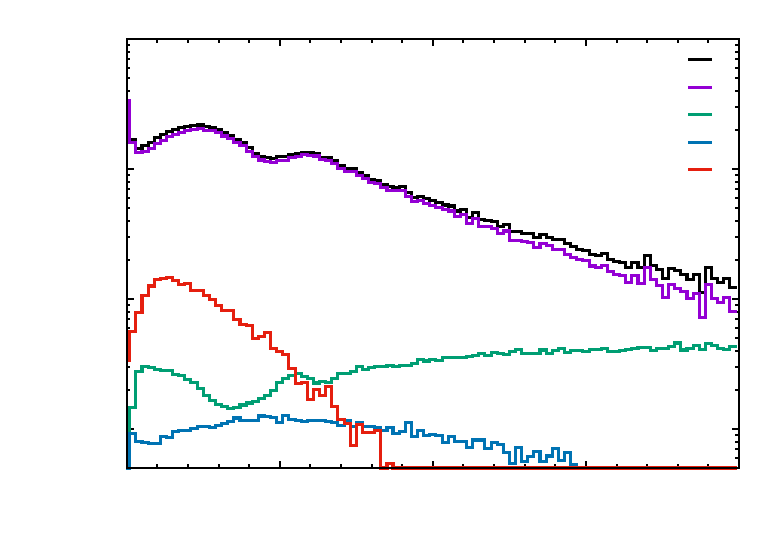
\includegraphics{pics/fluxnubar}}%
    \gplfronttext
  \end{picture}%
\endgroup
}
	\hspace{-1em}
	\resizebox{.5\textwidth}{!}{% GNUPLOT: LaTeX picture with Postscript
\begingroup
  \makeatletter
  \providecommand\color[2][]{%
    \GenericError{(gnuplot) \space\space\space\@spaces}{%
      Package color not loaded in conjunction with
      terminal option `colourtext'%
    }{See the gnuplot documentation for explanation.%
    }{Either use 'blacktext' in gnuplot or load the package
      color.sty in LaTeX.}%
    \renewcommand\color[2][]{}%
  }%
  \providecommand\includegraphics[2][]{%
    \GenericError{(gnuplot) \space\space\space\@spaces}{%
      Package graphicx or graphics not loaded%
    }{See the gnuplot documentation for explanation.%
    }{The gnuplot epslatex terminal needs graphicx.sty or graphics.sty.}%
    \renewcommand\includegraphics[2][]{}%
  }%
  \providecommand\rotatebox[2]{#2}%
  \@ifundefined{ifGPcolor}{%
    \newif\ifGPcolor
    \GPcolortrue
  }{}%
  \@ifundefined{ifGPblacktext}{%
    \newif\ifGPblacktext
    \GPblacktexttrue
  }{}%
  % define a \g@addto@macro without @ in the name:
  \let\gplgaddtomacro\g@addto@macro
  % define empty templates for all commands taking text:
  \gdef\gplbacktext{}%
  \gdef\gplfronttext{}%
  \makeatother
  \ifGPblacktext
    % no textcolor at all
    \def\colorrgb#1{}%
    \def\colorgray#1{}%
  \else
    % gray or color?
    \ifGPcolor
      \def\colorrgb#1{\color[rgb]{#1}}%
      \def\colorgray#1{\color[gray]{#1}}%
      \expandafter\def\csname LTw\endcsname{\color{white}}%
      \expandafter\def\csname LTb\endcsname{\color{black}}%
      \expandafter\def\csname LTa\endcsname{\color{black}}%
      \expandafter\def\csname LT0\endcsname{\color[rgb]{1,0,0}}%
      \expandafter\def\csname LT1\endcsname{\color[rgb]{0,1,0}}%
      \expandafter\def\csname LT2\endcsname{\color[rgb]{0,0,1}}%
      \expandafter\def\csname LT3\endcsname{\color[rgb]{1,0,1}}%
      \expandafter\def\csname LT4\endcsname{\color[rgb]{0,1,1}}%
      \expandafter\def\csname LT5\endcsname{\color[rgb]{1,1,0}}%
      \expandafter\def\csname LT6\endcsname{\color[rgb]{0,0,0}}%
      \expandafter\def\csname LT7\endcsname{\color[rgb]{1,0.3,0}}%
      \expandafter\def\csname LT8\endcsname{\color[rgb]{0.5,0.5,0.5}}%
    \else
      % gray
      \def\colorrgb#1{\color{black}}%
      \def\colorgray#1{\color[gray]{#1}}%
      \expandafter\def\csname LTw\endcsname{\color{white}}%
      \expandafter\def\csname LTb\endcsname{\color{black}}%
      \expandafter\def\csname LTa\endcsname{\color{black}}%
      \expandafter\def\csname LT0\endcsname{\color{black}}%
      \expandafter\def\csname LT1\endcsname{\color{black}}%
      \expandafter\def\csname LT2\endcsname{\color{black}}%
      \expandafter\def\csname LT3\endcsname{\color{black}}%
      \expandafter\def\csname LT4\endcsname{\color{black}}%
      \expandafter\def\csname LT5\endcsname{\color{black}}%
      \expandafter\def\csname LT6\endcsname{\color{black}}%
      \expandafter\def\csname LT7\endcsname{\color{black}}%
      \expandafter\def\csname LT8\endcsname{\color{black}}%
    \fi
  \fi
    \setlength{\unitlength}{0.0500bp}%
    \ifx\gptboxheight\undefined%
      \newlength{\gptboxheight}%
      \newlength{\gptboxwidth}%
      \newsavebox{\gptboxtext}%
    \fi%
    \setlength{\fboxrule}{0.5pt}%
    \setlength{\fboxsep}{1pt}%
\begin{picture}(7200.00,5040.00)%
    \gplgaddtomacro\gplbacktext{%
      \csname LTb\endcsname%%
      \put(924,704){\makebox(0,0)[r]{\strut{}\np{1}}}%
      \put(924,1733){\makebox(0,0)[r]{\strut{}\np{10}}}%
      \put(924,2762){\makebox(0,0)[r]{\strut{}\np{e2}}}%
      \put(924,3790){\makebox(0,0)[r]{\strut{}\np{e3}}}%
      \put(924,4819){\makebox(0,0)[r]{\strut{}\np{e4}}}%
      \put(1056,484){\makebox(0,0){\strut{}0}}%
      \put(2526,484){\makebox(0,0){\strut{}5}}%
      \put(3996,484){\makebox(0,0){\strut{}10}}%
      \put(5465,484){\makebox(0,0){\strut{}15}}%
      \put(6935,484){\makebox(0,0){\strut{}20}}%
    }%
    \gplgaddtomacro\gplfronttext{%
      \csname LTb\endcsname%%
      \put(308,2761){\rotatebox{-270}{\makebox(0,0){\strut{}$\overset{(-)}{\nu}_\tau / \text{cm}^2 / \text{GeV}$}}}%
      \put(3995,154){\makebox(0,0){\strut{}Energy (GeV)}}%
      \csname LTb\endcsname%%
      \put(6318,4624){\makebox(0,0)[r]{\strut{}$D_s\to\nu_\tau$}}%
      \csname LTb\endcsname%%
      \put(6318,4360){\makebox(0,0)[r]{\strut{}$\tau\to\cj{\nu}_\tau e$}}%
      \csname LTb\endcsname%%
      \put(6318,4096){\makebox(0,0)[r]{\strut{}$\tau\to\cj{\nu}_\tau \mu$}}%
      \csname LTb\endcsname%%
      \put(6318,3832){\makebox(0,0)[r]{\strut{}$\tau\to\cj{\nu}_\tau \pi$}}%
      \csname LTb\endcsname%%
      \put(6318,3568){\makebox(0,0)[r]{\strut{}$\tau\to\cj{\nu}_\tau \pi\pi^0$}}%
    }%
    \gplbacktext
    \put(0,0){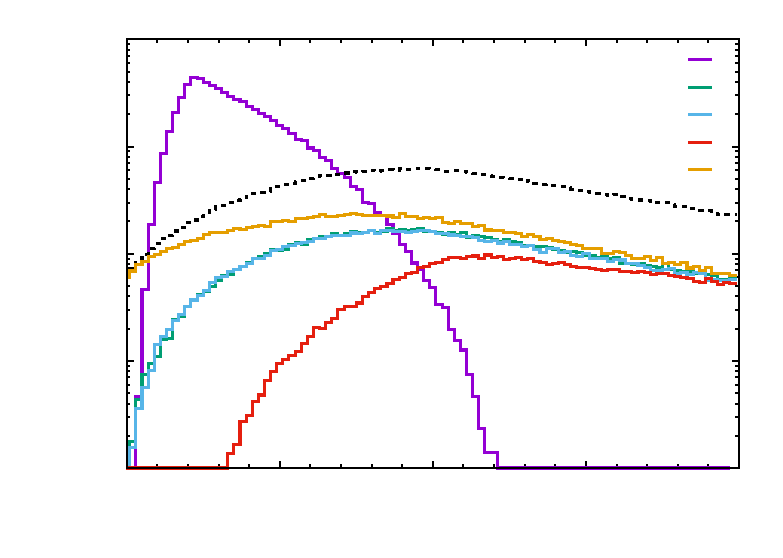
\includegraphics{pics/fluxnutau}}%
    \gplfronttext
  \end{picture}%
\endgroup
}
	\caption{The prediction of neutrino fluxes, in neutrino mode, divided by parentage at the ND are shown above, %
		normalised to \np{e20}\,POT.
		The $\nu_e$ component (top left) predominately originates from $\mu^+$ decays;
		kaon decays are responsible for the high energy part of the spectrum.
		The $\nu_\mu$ component (top right) obtains its main contribution from $\pi^+$ decays at low energies, %
		whereas the $K^+$ decays are accountable for the long tail of the spectrum.
		Contributions from $D_s^+$ decay are out of scale for both $\nu_e$ and $\nu_\mu$.
		The distribution of the $\cj{\nu}_\mu$ component (bottom left) is due to %
		negative charged secondary particles which are not successfully deflected by the horn system;
		the muon contribution is much more relevant than for the $\nu_\mu$ component.
		The $\nu_\tau$ component (bottom right) is only sourced from $D_s$ decays and presents a prominent peak at low energies, %
		whereas the $\cj{\nu}_\tau$ are produced in $\tau^+$ lepton decays.
		The dotted black line is the total $\cj{\nu}_\tau$ component of the flux.}
	\label{fig:fluxes}
\end{figure}

%A powerful proton beam is responsible for the very intense neutrino flux at the LBNF facility.
In order to implement our analysis, the various components of the flux by parentage must be known separately.
We study only the beam operating with a forward horn current, which selects %
positively charged secondary particles and results in a beam dominantly made of neutrinos %
with a smaller component of antineutrinos.
%
The flux predictions for $\nu_e$, $\nu_\mu$, and $\cj{\nu}_\mu$, provided by \refref{LauraFields} for the reference beam, %
are shown in~\reffig{fig:fluxes} subdivided in their parent components.
The $\nu_\mu$ flux is the dominant component and is principally originated %
by pion decays, whilst its long tail comes from kaon decays.
Unsuccessfully deflected negative particles, like $\pi^-$ or $K^-$, and the $\mu^+$ are the main contributors %
to the $\cj{\nu}_\mu$ components, and $\nu_e$ comes predominately from the muon %
and both $K^+$ and $K^0$ decays.
We consider only the energy range $E < 20\,\text{GeV}$, because it is the most intense region of the flux %
and, as it will be explained in~\refsec{sec:numevt}, the most relevant for this study.

\begin{figure}[t]
	\centering
	\resizebox{\linewidth}{!}{% GNUPLOT: LaTeX picture with Postscript
\begingroup
  \makeatletter
  \providecommand\color[2][]{%
    \GenericError{(gnuplot) \space\space\space\@spaces}{%
      Package color not loaded in conjunction with
      terminal option `colourtext'%
    }{See the gnuplot documentation for explanation.%
    }{Either use 'blacktext' in gnuplot or load the package
      color.sty in LaTeX.}%
    \renewcommand\color[2][]{}%
  }%
  \providecommand\includegraphics[2][]{%
    \GenericError{(gnuplot) \space\space\space\@spaces}{%
      Package graphicx or graphics not loaded%
    }{See the gnuplot documentation for explanation.%
    }{The gnuplot epslatex terminal needs graphicx.sty or graphics.sty.}%
    \renewcommand\includegraphics[2][]{}%
  }%
  \providecommand\rotatebox[2]{#2}%
  \@ifundefined{ifGPcolor}{%
    \newif\ifGPcolor
    \GPcolortrue
  }{}%
  \@ifundefined{ifGPblacktext}{%
    \newif\ifGPblacktext
    \GPblacktexttrue
  }{}%
  % define a \g@addto@macro without @ in the name:
  \let\gplgaddtomacro\g@addto@macro
  % define empty templates for all commands taking text:
  \gdef\gplbacktext{}%
  \gdef\gplfronttext{}%
  \makeatother
  \ifGPblacktext
    % no textcolor at all
    \def\colorrgb#1{}%
    \def\colorgray#1{}%
  \else
    % gray or color?
    \ifGPcolor
      \def\colorrgb#1{\color[rgb]{#1}}%
      \def\colorgray#1{\color[gray]{#1}}%
      \expandafter\def\csname LTw\endcsname{\color{white}}%
      \expandafter\def\csname LTb\endcsname{\color{black}}%
      \expandafter\def\csname LTa\endcsname{\color{black}}%
      \expandafter\def\csname LT0\endcsname{\color[rgb]{1,0,0}}%
      \expandafter\def\csname LT1\endcsname{\color[rgb]{0,1,0}}%
      \expandafter\def\csname LT2\endcsname{\color[rgb]{0,0,1}}%
      \expandafter\def\csname LT3\endcsname{\color[rgb]{1,0,1}}%
      \expandafter\def\csname LT4\endcsname{\color[rgb]{0,1,1}}%
      \expandafter\def\csname LT5\endcsname{\color[rgb]{1,1,0}}%
      \expandafter\def\csname LT6\endcsname{\color[rgb]{0,0,0}}%
      \expandafter\def\csname LT7\endcsname{\color[rgb]{1,0.3,0}}%
      \expandafter\def\csname LT8\endcsname{\color[rgb]{0.5,0.5,0.5}}%
    \else
      % gray
      \def\colorrgb#1{\color{black}}%
      \def\colorgray#1{\color[gray]{#1}}%
      \expandafter\def\csname LTw\endcsname{\color{white}}%
      \expandafter\def\csname LTb\endcsname{\color{black}}%
      \expandafter\def\csname LTa\endcsname{\color{black}}%
      \expandafter\def\csname LT0\endcsname{\color{black}}%
      \expandafter\def\csname LT1\endcsname{\color{black}}%
      \expandafter\def\csname LT2\endcsname{\color{black}}%
      \expandafter\def\csname LT3\endcsname{\color{black}}%
      \expandafter\def\csname LT4\endcsname{\color{black}}%
      \expandafter\def\csname LT5\endcsname{\color{black}}%
      \expandafter\def\csname LT6\endcsname{\color{black}}%
      \expandafter\def\csname LT7\endcsname{\color{black}}%
      \expandafter\def\csname LT8\endcsname{\color{black}}%
    \fi
  \fi
    \setlength{\unitlength}{0.0500bp}%
    \ifx\gptboxheight\undefined%
      \newlength{\gptboxheight}%
      \newlength{\gptboxwidth}%
      \newsavebox{\gptboxtext}%
    \fi%
    \setlength{\fboxrule}{0.5pt}%
    \setlength{\fboxsep}{1pt}%
\begin{picture}(14400.00,5040.00)%
    \gplgaddtomacro\gplbacktext{%
      \csname LTb\endcsname%%
      \put(444,440){\makebox(0,0)[r]{\strut{}\np{10}}}%
      \put(444,1509){\makebox(0,0)[r]{\strut{}\np{e2}}}%
      \put(444,2579){\makebox(0,0)[r]{\strut{}\np{e3}}}%
      \put(444,3648){\makebox(0,0)[r]{\strut{}\np{e4}}}%
      \put(444,4717){\makebox(0,0)[r]{\strut{}\np{e5}}}%
      \put(576,220){\makebox(0,0){\strut{}$0$}}%
      \put(2336,220){\makebox(0,0){\strut{}$5$}}%
      \put(4095,220){\makebox(0,0){\strut{}$10$}}%
    }%
    \gplgaddtomacro\gplfronttext{%
      \csname LTb\endcsname%%
      \put(-172,2739){\rotatebox{-270}{\makebox(0,0){\strut{}$\nu_\tau$/cm\tapi{2}/GeV}}}%
      \put(2687,-110){\makebox(0,0){\strut{}Energy (GeV)}}%
      \csname LTb\endcsname%%
      \put(4182,4844){\makebox(0,0)[r]{\strut{}0 MeV}}%
      \csname LTb\endcsname%%
      \put(4182,4580){\makebox(0,0)[r]{\strut{}100 MeV}}%
      \csname LTb\endcsname%%
      \put(4182,4316){\makebox(0,0)[r]{\strut{}150 MeV}}%
      \csname LTb\endcsname%%
      \put(4182,4052){\makebox(0,0)[r]{\strut{}180 MeV}}%
      \csname LTb\endcsname%%
      \put(4182,3788){\makebox(0,0)[r]{\strut{}190 MeV}}%
    }%
    \gplgaddtomacro\gplbacktext{%
      \csname LTb\endcsname%%
      \put(5820,440){\makebox(0,0)[r]{\strut{}0.8}}%
      \put(5820,1590){\makebox(0,0)[r]{\strut{}0.85}}%
      \put(5820,2740){\makebox(0,0)[r]{\strut{}0.9}}%
      \put(5820,3889){\makebox(0,0)[r]{\strut{}0.95}}%
      \put(5820,5039){\makebox(0,0)[r]{\strut{}1}}%
      \put(5952,220){\makebox(0,0){\strut{}$0$}}%
      \put(6936,220){\makebox(0,0){\strut{}$0.5$}}%
      \put(7920,220){\makebox(0,0){\strut{}$1$}}%
      \put(8903,220){\makebox(0,0){\strut{}$1.5$}}%
      \put(9887,220){\makebox(0,0){\strut{}$2$}}%
    }%
    \gplgaddtomacro\gplfronttext{%
      \csname LTb\endcsname%%
      \put(5072,2739){\rotatebox{-270}{\makebox(0,0){\strut{}Factor}}}%
      \put(7919,-110){\makebox(0,0){\strut{}Mass $m_N$ (GeV)}}%
      \csname LTb\endcsname%%
      \put(9270,4844){\makebox(0,0)[r]{\strut{}$\tau \to \cj{\nu}_\tau e$}}%
      \csname LTb\endcsname%%
      \put(9270,4580){\makebox(0,0)[r]{\strut{}$\tau \to \cj{\nu}_\tau \mu$}}%
      \csname LTb\endcsname%%
      \put(9270,4316){\makebox(0,0)[r]{\strut{}$\tau \to \cj{\nu}_\tau \pi$}}%
      \csname LTb\endcsname%%
      \put(9270,4052){\makebox(0,0)[r]{\strut{}$\tau \to \cj{\nu}_\tau \pi \pi^0$}}%
    }%
    \gplgaddtomacro\gplbacktext{%
      \csname LTb\endcsname%%
      \put(10332,440){\makebox(0,0)[r]{\strut{}0}}%
      \put(10332,1276){\makebox(0,0)[r]{\strut{}0.2}}%
      \put(10332,2112){\makebox(0,0)[r]{\strut{}0.4}}%
      \put(10332,2949){\makebox(0,0)[r]{\strut{}0.6}}%
      \put(10332,3785){\makebox(0,0)[r]{\strut{}0.8}}%
      \put(10332,4621){\makebox(0,0)[r]{\strut{}1}}%
      \put(10464,220){\makebox(0,0){\strut{}$0$}}%
      \put(11448,220){\makebox(0,0){\strut{}$0.5$}}%
      \put(12432,220){\makebox(0,0){\strut{}$1$}}%
      \put(13415,220){\makebox(0,0){\strut{}$1.5$}}%
      \put(14399,220){\makebox(0,0){\strut{}$2$}}%
    }%
    \gplgaddtomacro\gplfronttext{%
      \csname LTb\endcsname%%
      \put(12431,-110){\makebox(0,0){\strut{}Mass $m_N$ (GeV)}}%
      \csname LTb\endcsname%%
      \put(13782,4844){\makebox(0,0)[r]{\strut{}$\tau \to \cj{\nu}_\tau e$}}%
      \csname LTb\endcsname%%
      \put(13782,4580){\makebox(0,0)[r]{\strut{}$\tau \to \cj{\nu}_\tau \mu$}}%
      \csname LTb\endcsname%%
      \put(13782,4316){\makebox(0,0)[r]{\strut{}$\tau \to \cj{\nu}_\tau \pi$}}%
      \csname LTb\endcsname%%
      \put(13782,4052){\makebox(0,0)[r]{\strut{}$\tau \to \cj{\nu}_\tau \pi \pi^0$}}%
    }%
    \gplbacktext
    \put(0,0){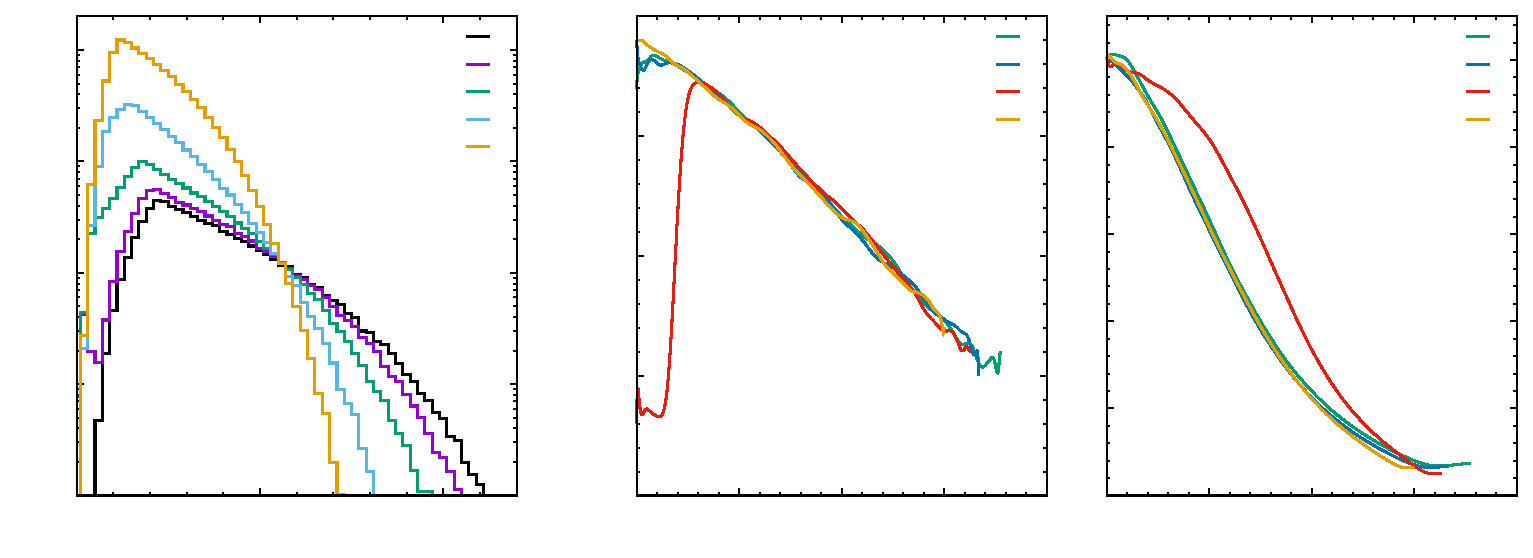
\includegraphics{pics/modmulti}}%
    \gplfronttext
  \end{picture}%
\endgroup
}
	\caption{The fluxes of heavy neutrinos from $D_s^+\to \tau^+ N$ (left) are presented %
		for different neutrino masses and normalised to \np{e20}~POT at the ND.
		Only phase space effects are considered here.
		For each different value of the neutrino mass, information on the start and end point of the spectrum %
		and the peak of the flux are extracted and used to reshape the $\nu_\tau$ spectrum.
		We show the distortion factors used in the scaling process for the channel producing $\cj{\nu}_\tau$: %
		the energy range normalised to 20\,GeV (middle) and the inverse of the peak re-scaling (right). }
	\label{fig:taudist}
\end{figure}

We highlight here the fact that we expect also an albeit-small flux of HNLs with masses above the kaon one.
This could be inferred from the $\nu_\tau$ flux, but this is not available in the literature.
In fact, the lightest meson with an interesting decay width to tau neutrinos is the charmed-strange meson~$D_s^+$, %
which has a mass $m_{D_s} = \np{1968.34}\pm\np{0.07}$\,MeV~\cite{PDG}.
It~decays into $\tau^+ \nu_\tau$ with a branching ratio of $\np{5.48}\pm\np{0.23}$\,\%.
HNL with masses above the $K^0$ can be produced via the tau mixing, but more importantly via %
the muonic and electronic ones which are enhanced, as shown in \refsec{sec:production}.
The meson $D^+$ also decays into $\tau^+ \nu_\tau$, but being lighter than the $D_s^+$, %
the decay is disfavoured by the smaller phase space, with a branching ratio~50 times smaller.
This meson presents three-body decay channels into $\nu_e$ and $\nu_\mu$ with much higher branching ratio, %
but there is no enhancement for such channels into HNL, as explained in \refsec{sec:production}, and so these subdominant components %
are not taken in account in the present study.

%However, HNL with masses above the $K^0$ mass can only be produced by the decays of $D^+$ and $D_s^+$, %
%and the production of massive neutrinos could be enhanced, especially if produced via the $|U_{e 4}|^2$ mixing.
%{\color{red} What about the decay of $D^+$?? The considerations of it being disfavoured because of phase space would not apply to decay into N and muons or N and electron, which are enhanced compared to the standard case.}
%We make an estimate of the $\nu_\tau$ spectrum, starting from the $D_s^+$ production by %
%an 80\,GeV proton beam hitting a fixed graphite target.
The proton beam has a relatively low energy for producing charm quarks with a high cross-section, %
so the prediction of $\nu_\tau$ has not been carried out by the collaboration to the best of our knowledge.
For the reasons stated above, we make a prediction for the $D_s^+$ production by %
an 80\,GeV proton beam hitting a fixed graphite target.
The distribution at the production site will be then used to estimate the $\nu_\tau$ flux at the ND system.
In the literature, the following parametrisation has been successfully used to describe %
the charm meson production in proton-proton collision in the Centre of Mass frame~\cite{Ammar:1988ta}
\begin{equation}
	\label{eq:dsflux}
	\frac{\dd[2]{\sigma}}{\dd{x_F}\dd{p_T^2}} \sim (1-|x_F|)^n e^{-b p_T^2}~,
\end{equation}
where $x_F = 2 p_z/\sqrt{s}$, with $p_z$ the longitudinal momentum in the CM frame. %
The parameters $n$ and $b$ were fitted from the E769 experiment and found to be %
$n = \np{6.1}\pm\np{0.7}$ and \mbox{$b = \np{1.08}\pm\np{0.09}$}~\cite{Alves:1996qz}.
We assume that the $D_s^+$ meson production at the target follows the same distribution.
With the help of a Monte Carlo simulation, we generate the $D_s^+$ four-momenta starting from~\refeq{eq:dsflux} %
and simulate the meson decay and the subsequent tau decays.
A key simplification here is that because of the short lifetime of the $D_s^+$ and $\tau^+$, %
of the order of \np{e-13}\,s, their path is not affected by the horn system nor by interactions with other accelerator components. 
This results in no focusing of these secondary particles, and so only neutrinos emitted %
within the geometric acceptance of the ND are considered to form the $\nu_\tau$ and $\cj{\nu}_\tau$ spectrum.
The overall normalisation comes from an open charm calculation (see~\refapp{sec:opencc} for details): %
the number of $D_s^+$ per POT is found to be $(2.8 \pm 0.2) \times \np{e-6}$.
The result of the simulation is reported in the bottom right panel of~\reffig{fig:fluxes}, %
where the different contributions to the $\nu_\tau$ spectrum are shown.
Thanks to the large number of POTs in DUNE, the total number of $D_s^+$ mesons produced is comparable %
to other dedicated experiments~\cite{Alekhin:2015byh}; %
however, the beamline design is not optimised for heavy mesons production %
and the $\nu_\tau$ flux seen at the ND is strongly attenuated.%: %
%according to our simulation, only \np{0.13}\,\% of the neutrinos produced at the target reaches the ND.

Having knowledge of the parent meson distribution, we directly simulate the production of nearly-sterile neutrinos %
from the $D_s$ decays.
The spectrum of heavy neutrinos is distorted when their mass approaches the various phase space thresholds, %
which appears as a further enhancement of the flux. 
This is because heavier neutrinos are more easily boosted inside the geometric acceptance of the detector.
Besides the peak height, the start and the end point of the energy flux are also affected,
as illustrated in~\reffig{fig:taudist}. 
We take these effects in account, modifying the scaled neutrino flux using information retrieved by the $\nu_\tau$ and $\cj{\nu}_\tau$~simulation. 

\subsection{Background evaluation}
\label{sec:background}

%The major source of noise comes from ordinary neutrino-nucleon interactions happening within the fiducial volume of the detector.
%As shown in~\reftab{tab:rate}, the ND will expect a copious number of CC and NC events. %, usually categorised as: %
%\begin{itemize}
%	\item Charged Current Quasi-Elastic (CCQE) interactions whether a charged lepton is present in the final state, %
%		revealing the flavour state of the incoming neutrino;
%	\item Neutral Current Elastic (NCE) scatterings if there is no charged lepton;
%	\item CC resonant pion production (CC1$\pi$) when a pion is also emitted;
%	\item NC resonant pion production (NC1$\pi$) if it is mediated by neutral currents;
%	\item Deep Inelastic Scattering (DIS) which classifies all interaction happening at high energy and with high level %
%	of hadronization.
%\end{itemize}

\begin{table}
	\newcommand{\us}{\hphantom{${}^0$}}
	\newcommand{\ms}{\hphantom{${}^-$}}
	\centering
	\small
	\iffalse
	\begin{tabular}{lrrrrrr}
		\toprule
		& \multicolumn{3}{c}{CC events}	&  \multicolumn{3}{c}{NC events}	\\
		%\midrule
		\cmidrule(lr){2-4} \cmidrule(lr){5-7}
		& Per tonne	& Ratio		& Rate (Hz)	& Per tonne 	& Ratio	& Rate (Hz)	\\
		\cmidrule(lr){2-4} \cmidrule(lr){5-7}
		%\midrule
		$\nu_e$		    & \np{3.0e3}\ms	& 75.6\,\%	& \np{152e-3}\us& \np{1.0e3}\ms	& 24.4\,\%	& \np{48.9e-3}\us	\\
		$\nu_\mu$	    & \np{236e3}\ms	& 75.2\,\%	& \np{12.0e0}\ms\us& \np{77.8e3}\ms& 24.8\,\%	& \np{3.95e0}\ms\us	\\
		$\cj{\nu_\mu}$	& \np{17.7e3}\ms& 70.9\,\%	& \np{898e-3}\us	& \np{7.2e3}\ms	& 29.1\,\%	& \np{368e-3}\us	\\
		$\nu_\tau$	    & \np{1.6e-5}	& 17.1\,\%	& \np{8.3e-10}	& \np{7.9e-5}	& 82.9\,\%	& \np{4.0e-10}	\\
		$\cj{\nu_\tau}$	& \np{5.2e-5}	& 45.3\,\%	& \np{2.6e-9}\us	& \np{6.1e-5}	& 54.7\,\%	& \np{3.0e-9}\us	\\
		\bottomrule
	\end{tabular}
	\fi
	\begin{tabular}{lrrr@{\,}lrrr@{\,}l} 
		\toprule
		& \multicolumn{3}{c}{CC events}	&  \multicolumn{3}{c}{NC events}	\\
		%\midrule
		\cmidrule(lr){2-5} \cmidrule(lr){6-9}
		& Per tonne	& Ratio		& \multicolumn{2}{c}{Rate (Hz)}	& Per tonne 	& Ratio	& \multicolumn{2}{c}{Rate (Hz)}	\\
		\cmidrule(lr){2-5} \cmidrule(lr){6-9}
		%\midrule
	$\nu_e$		    & %
	\np{3.0e3}\ms	& 75.6\,\%	& 152  & $\times\,10^{-3}$ & \np{1.0e3}\ms  & 24.4\,\% & 48.9 & $\times\,10^{-3}$	\\
	$\nu_\mu$	    & %
	\np{236e3}\ms	& 75.2\,\%	& 12.0 &                 & \np{77.8e3}\ms & 24.8\,\% & 3.95 &                  	\\
	$\cj{\nu_\mu}$	& %
	\np{17.7e3}\ms& 70.9\,\%	& 898  & $\times\,10^{-3}$ & \np{7.2e3}\ms  & 29.1\,\% & 368 & $\times\,10^{-3}$	\\
	$\nu_\tau$	    & %
	\np{1.6e-5}	& 17.1\,\%      & 8.3  & $\times\,10^{-10}$& \np{7.9e-5}    & 82.9\,\% & 4.0 & $\times\,10^{-10}$	\\
	$\cj{\nu_\tau}$	& %
	\np{5.2e-5}	& 45.3\,\%      & 2.6  & $\times\,10^{-3}$ & \np{6.1e-5}    & 54.7\,\% & 3.0 & $\times\,10^{-9}$	\\
		\bottomrule
	\end{tabular}
	\caption{The expected rates for CC and NC interaction in the near detector are presented here, normalised to %
		\np{e20}\,POT.
		The values were computed starting from~\refeq{eq:numev}, convolving the fluxes of~\reffig{fig:fluxes} 
		with the CC and NC cross section predictions from \textsc{genie}~\cite{Andreopoulos:2009rq}.
		Detector efficiencies are not applied.
		The first columns show the total number of events per tonne of argon, the second ones %
		the proportion of CC or NC events with respect to the totality, and the last columns the event frequencies %
		assuming \np{1e14}\,POT/s.}
	\label{tab:rate}
\end{table}

The number of SM neutrino--nucleon interactions expected at the DUNE ND, without considering detector effects, is calculated %
by integrating the Charged Current (CC) and Neutral Current (NC) total cross sections multiplied %
by the light neutrino spectrum~$\dv*{\phi_\nu}{E}$:
\begin{equation}
	\label{eq:numev}
	\mathcal{N}_\text{tot} = \mathcal{N}_\text{CC} + \mathcal{N}_\text{NC} = 
	\mathcal{N}_\text{target} \int \dd{E} \qty[\sigma_\text{CC}(E) + \sigma_\text{NC}(E)] \, \dv{\phi_\nu}{E}\ ,
\end{equation}
where $\sigma_\text{CC}(E)$ and $\sigma_\text{NC}(E)$ are the cross section predictions in argon %
calculated with \mbox{\textsc{genie}}~\cite{Andreopoulos:2009rq}, and $\mathcal{N}_\text{target}$ is the %
total number of Ar targets. 
The event rates are shown in~\reftab{tab:rate}.
It turns out that less than one $\nu_\tau$ event is expected in the total run of the experiment.
As~a~comparison, the number of $\nu_\mu$ events will be \np{e10} times higher.
This confirms the expectations that the $\nu_\tau$ component of the flux is negligible %
for standard oscillation physics in~DUNE ND.
On the other hand $\nu_\tau$ appearance is expected at the FD.


%%%% START EDIT

These neutrino scatterings occurring within the fiducial volume of the detector could mimic %
the rare signal of neutrino in-flight decays, as some final state particles are common to both processes.
A good estimate of the number of possible background events for each discovery channel is very important, %
since it dictates the true sensitivity of the experiment.
We restrict our conservative background analysis to decay modes available for neutrino masses below $m_{K^0}$, %
being these the channels with the best discovery potential.
They are $N\to\nu e^+ e^-$, $\nu e^\pm \mu^\mp$, $\nu \mu^+ \mu^-$, $\nu \pi^0$, $e^\mp \pi^\pm$, and $\mu^\mp \pi^\pm$.
%
Particles are typically tagged by studying the topology of the tracks and the energy loss $\dv*{E}{x}$ in the active medium, %
but instead of dealing with a full detector simulation, we perform a fast Monte Carlo analysis, %
using as input neutrino--nucleon scattering events in argon generated by the neutrino event generator \textsc{genie}~\cite{Andreopoulos:2009rq}.
The tracks are randomly placed inside the ND system and then smeared according to a normal distribution centred on the simulated value of energy/momentum; %
particles with a kinetic energy above the detection threshold are then assumed to be reconstructed.
%
The relative position between the two detectors is taken into account, in that %
particle tracks exiting the LArTPC end entering the MPD are reconstructed as a single track.
Escaping or partially reconstructed tracks are not discarded, but treated with a different energy/momentum resolution: %
the initial particle energy can be estimated, with some limitations, thanks to the energy dependence of the mean energy loss %
during the particle propagation.
We then implement possible sources of background mis-identification which are channel specific.
Detector resolutions and thresholds, from~\refref{Alion:2016uaj} for both parts of the ND, are summarised in~\reftab{tab:fastmc}.

%\clearpage

\begin{table}
	\centering
	\small
	\begin{tabular}{lccc}
		\toprule
		Particle& Threshold	& $\sigma_\text{rel}$	&  $\sigma_\theta$		\\
		\midrule
		EM	& 30\,MeV	& $5\%/\sqrt{E} \oplus 1\%$	& 1\textdegree	\\
		Hadron	& 50\,MeV	& $30\%/\sqrt{E} \oplus 5\%$	& 5\textdegree	\\
		Muon	& 30\,MeV	& 1\% or 30\% of $|\vb{p}|$	& 0.3\textdegree	\\
		Pion	& 100\,MeV	& 1\% or 30\% of $|\vb{p}|$	& 0.3\textdegree	\\
		\bottomrule
	\end{tabular}
	\caption{The table lists detection thresholds and energy/momentum and angular resolutions used in the fast MC, %
		where ``EM'' delineates electro-magnetic showers and ``Hadron'' any other charged particle %
		which is neither a lepton nor a pion.
		The momenta of pions and muons are smeared according to the containment of their tracks.
		If the particles enter the MPD in which they cover a length longer than the detector's diameter or %
		if 80\,\% of the tracks are contained inside the LArTPC then the relative resolution on the momentum is 5\,\%, %
		otherwise a resolution of 30\,\% is applied.
		Neutrons are treated with ``Hadron'' resolutions, but with a 90\,\% detection efficiency. }
	\label{tab:fastmc}
\end{table}
%
A strong discriminant for background events is the presence of protons, neutrons, and other hadrons in the final states, %
which are the results of the nucleus recoil of the neutrino interaction.
%If the nucleon or nucleus recoil in a neutrino-nucleon interaction can be identified, %
If hadronic activity is reconstructed as an interaction vertex, then the event is clearly originated by %
SM neutrino--nucleon scattering and tagged as background.
In the case this does not happen, for instance when the hadrons are below threshold, the multiplicity of final state particles %
becomes fundamental to distinguish signal events from intrinsic background.
However, this background can be worsened by mis-identification of certain tracks.

The main background to the pseudo-scalar meson channels, $N\to \ell^\mp \pi^\pm$, are resonance $\nu_e$ or $\nu_\mu$--CC %
interaction with single pion production or charged current incoherent and deep inelastic scatterings %
in which only a pair $\ell\,\pi$ is detected.
Three-body lepton decays suffers from mis-identification of additional pions and photons emitted in CC neutrino scatterings %
which are mistaken for charged leptons.
Despite having a similar mass, pion and muon tracks differ on average in length, as the meson track often culminates in a hadronic shower.
In~our implementation of the detector effects, if no hadronic shower is detected and the track length is longer than two metres, %
the pion is identified as a muon.
Electromagnetic shower induced by photons are identified by looking at the vertex displacement and at the $\dv*{E}{x}$, %
which is twice as large as the energy loss for $e^\pm$.
If a photon converts within two centimetres from the interaction point, and either the electron or the positron of the pair is below threshold, %
the photon is reconstructed as a single electron.
%assuming the other electron of the pair doesn't shower or is below threshold.
A pair of electrons with a small separation angle, less than 3\textdegree, is tagged as an electron-positron pair %
and the parent photon is reconstructed.
The main source of photons comes from the decay of the neutral pion, which is abundantly produced in %
NC neutrino--nucleon interactions.
Certain hadronic transitions from secondary particles of deep inelastic scatterings also emit gammas.
If a pair of photons shows an invariant mass comparable with the $\pi^0$ mass, the parent pion is identified.
Interactions in which multiple neutral pions are produced, but only a pair of photons is detected and reconstructed, %
are background to the $N\to \nu \pi^0$ channel.
The~background events surviving particle identification are between 2.5\,\% down to 0.0025\,\% of the processed events.
%the rejection of which strongly depends on the analysed channel.

%A million neutrino-nucleon events in argon is generated using the neutrino event generator \textsc{genie}~\cite{Andreopoulos:2009rq} %
%and then smeared according to a normal distribution centred on the simulated value of energy/momentum: %
%%{\color{red} true value of what? energy??} %
%particles with a kinetic energy above the detection threshold are assumed to be reconstructed.
%We use the same resolutions and thresholds from~\refref{Alion:2016uaj} for both parts of the ND.
%These are summarised in~\reftab{tab:fastmc}.
%We then implement detector geometry effects and possible sources of misidentification.
%{\color{red} but wouldn't it appear as 2 electrons???} 
%Likewise, if a pair of photons shows an invariant mass comparable with the $\pi^0$ mass, %
%the parent pion is identified.
%{color{red} WHAT DO WE MEAN WITH THIS????? Relying solely on particle counting,} the background is reduced by at least a factor of $\sim$10 %
%and up to a factor of $\sim\np{e4}$.

The channels which open up for masses above the kaon mass are more challenging from an experimental point of view.
The final state particles of these modes are mostly neutral pseudo-scalar mesons, which decay electromagnetically, %
or vector mesons, which usually decay into a multi-state of lighter mesons, depending on the initial flavour content,
sometimes accompanied by photon emission.
The correct identification of these short-lived states is non trivial.
For very high masses, also $\tau$ leptons are yielded, but their precise reconstruction requires \emph{ad hoc} techniques.
These tasks are beyond the scope of the analysis presented here and are best left to the collaboration superior simulation tools.
We also do not consider cosmogenic background, even though a rate of \np{2.7}\,Hz/m\tapi{2} cosmic rays %
is expected at the ND hall~\cite{Sinclair:DUNEdoc}, which has very little over burden.
Given an area of a few square meters, the number of cosmic rays per drift window can be non-negligible~\cite{Abi:2018dnh}, %
but rejection techniques are being developed with good signal efficiencies~\cite{Adams:2018lzd}.
%%% SOMETHING ON MUONS FROM BEAM? Comparing to ship active muon shield
%distinctive directionality compared to beam related events, and can be removed %
%using a veto detector installed at the top of the ND hall.


%\enlargethispage{\baselineskip}
%
\subsection{HNL decay events and signal efficiency}
\label{sec:numevt}

Except for $N$ decaying into three neutrinos, all the other decay channels are in principle detectable.
%Some decay modes contribute more significantly to the physics reach thanks to larger branching ratios and lower backgrounds.
%Along with the number of background events, a correct estimation of the number of decays in the visible channels %
%is necessary in order to evaluate the sensitivity of DUNE ND to the discovery of HNL.
%It is therefore fundamental to estimate the number of possible background events $\mathcal{B}_d$ for each channel $d$, %
For a given visible decay mode~$d$, the number of signal events is
%The expected number of heavy neutrino decays inside the detector for a given decay channel~$d$ %
%can be estimated with the following formula:
\begin{equation}
	\label{eq:event}
	\mathcal{N}_d = \int\!\! \dd{E}\ \Pi_d(E) W_d(E)\, \dv{\phi_N}{E}\ ,
\end{equation}
where $\dv*{\phi_N}{E}$ is the number of heavy neutrinos expected at the ND, %
computed in the way described in~\refsec{sec:production}.
The function $\Pi_d(E)$ accounts for the probability of a heavy neutrino of energy $E$ to decay inside the ND after covering the baseline distance $L$.
It is expressed in the following form:
\begin{equation}
	\Pi_d(E) = e^{-\frac{\Gamma_\text{tot} L}{\gamma \beta}} %
	\qty(1-e^{-\frac{\Gamma_\text{tot} \lambda}{\gamma \beta}}) \frac{\Gamma_d}{\Gamma_\text{tot}}\ , 
\end{equation}
where $\lambda$ is the length of the ND, $\Gamma_d$ the decay rate for the channel $d$ and %
$\Gamma_\text{tot}$ the total decay rate.
The total effect of $\Pi_d$ is to favour low-energy bins of the neutrino spectrum for which the %
relativistic factor $\gamma\beta$ is small.

The term $W_d(E)$ is a signal efficiency factor, estimated as the binned ratio of the true $N$ energy spectrum after %
and before a background rejection procedure.
This process aims at further reducing the number of background events still present after particle identification.
It consists of simple data selection cuts optimised to reject the background while keeping an acceptable signal efficiency %
($\geq 30\,\%$), exploiting differences in the energy and angular distributions between signal and background events.
The HNL decays inside the detector are simulated by a custom Monte Carlo code and the tracks are processed in the same way %
as it is done for background events (see~\refsec{sec:background}).
The resulting signal efficiency therefore embeds also detector effects.
If no background is expected for the channel $d$, there is no need for applying any rejection procedure %
and so the signal efficiency is maximal, i.e.\ $W_d(E) = 1$ at all energies.
The final number of background events $\mathcal{B}_d$ and the number of signal events $\mathcal{N}_d$ are %
eventually used to build the Confidence Level (C.L.) regions of sensitivity (see \refsec{sec:results}).
%
%The term $W_d(E)$ is a weighting factor given by thre binned ratio of the true $N$ energy spectrum after %
%and before the background reduction procedure.
%{\color{red} We discuss the backgrounds in the previous section. Why this stuff is here?} The latter process aims to further reduce the number of background events, still present after particle identification.
%It consists of simple data selection cuts optimised to reject the background while maintaining a high signal efficiency, %
%exploiting differences in the distributions of signal and background events.
%In general terms, background events are expected to have a more isotropic angular distribution %
%compared to decay-in-flight which are very boosted forward.	
%Signal events are generated with a custom Monte Carlo code and are processed in the same manner as the background events (see~\refsec{sec:background}).
%{\color{red} THE FOLLOWING IS NOT CLEAR In this way, the final weighting factor is the result of not only data selection cuts, but also detector effects.
%	If no background is expected before the event rejection process, then these factors are maximal, i.e.\ $W_d(E) = 1$ %
%	at all energies.
%	IS THAT SO?????? THE FOLLOWING IS NOT CLEAR EITHER. The final number of background events $\mathcal{B}_d$ is eventually used to define the Confidence Level (C.L.) regions of sensitivity.}
We leave a more detailed discussion on the background reduction cuts in~\refapp{sec:appbackground}, %
where we report the rates of background reduction and signal selection for all decay channels of both Majorana and Dirac neutrinos of a given mass.
%%%NOT TRUE ANYMORE 
%%%%
From our analysis, we note that selection cuts are slightly different for Dirac or Majorana HNL decays.
This is a consequence of certain combinations of production and decay modes which are forbidden for Dirac neutrinos, %
as they would lead to LNV, and so the energy and angular distributions are not identical.
NC--mediated decay mode have also intrinsically distinct decay widths in the heavy neutrino rest frame %
and the difference angular dependency can be reflected in the laboratory frame.
%We note that the selection cuts for Dirac neutrino decays are generally more strict than the corresponding %
%Majorana cuts for masses $m_N \gtrsim 0.25$.
%This results in less background for Dirac HNL decays, but also in a slightly worse signal efficiency.
%at rejecting background events for %
%expected HNL masses $m_N \gtrsim 0.25$ compared to the Majorana kinematic cuts.
%All decay rates not listed above are forbidden for a Dirac (anti-)particle %
%as the combination of production and decay would amount to a LNV process.
%The final true energy distributions of Majorana and Dirac neutrinos can therefore be different.
%When looking at the NC decay $N\to\nu \pi^0$, the difference in signal efficiency is almost recovered, %
%thanks to the angular dependence of Dirac neutrino decays which makes it more distinguishable from background.
%%%%

%This is a consequence of the different angular distribution between Majorana and Dirac neutrino decays.
%Because we are not taking in account charge identification in our analysis, Majorana neutrino decays are isotropic in the CM.
%{\color{red} THIS IS NOT CLEAR. In the case of Dirac neutrinos, there is a forward-backward asymmetry resulting from the unbalanced components of neutrinos and antineutrinos in the beam.
%	The difference in the angular distributions is slightly reflected in the laboratory frame and hence the signal efficiency can be affected.}

%	This can be seen as the limit in which the size of the detector $\lambda$ is %
%	greater than the decay length of the Majorana neutrino, $\beta \gamma\ \Gamma_\text{tot}^{\np{-1}}$, %
%	and the probability is approximated by
%	\begin{equation}
%		\Pi_d(E) \simeq e^{-\frac{\Gamma_\text{tot} L}{\gamma \beta}} \frac{\Gamma_d}{\Gamma_\text{tot}}\ .
%	\end{equation}
%	In this regime the event rate does not dependent on the detector size, as heavy neutrinos decay within a few %
%	decay lengths.

%The number of signal events is then compared to the expected number of background events.
%For a specific channel $d$, the probability of observing $n$ events with a signal mean $\sigma = \mathcal{N}_d$ %
%and background $b = \mathcal{B}_d$ follows a Poisson distribution:
%\begin{equation*}
%	P(n|\sigma,b) = (\sigma+b) \frac{e^{-(\sigma+b)}}{n!}\ .
%\end{equation*}
%The null hypothesis $H_0$ is that no sterile neutrino decays are seen ($\sigma = 0$), %
%while only background events $b$ are expected.
%We employ the Feldman and Cousins method~\cite{Feldman:1997qc} to estimate the number of events needed in order %
%to reject $H_0$ with the desired confidence level.
%For example, if no background is expected ($W_d = 1$), an average of $n = 2.44$ events %
%must be detected to reject $H_0$ with 90\,\% C.L.
%This criterion is used to define the sensitivity regions shown in~\refsec{sec:results} and~\ref{sec:combined}.
\section{Sensitivities of DUNE ND}
\label{sec:results}

We present here sensitivity regions for the discovery of heavy neutrino decays for %
a total amount of \np{1.32e22}\,POT collected with the beam in neutrino mode.
All the regions are estimated at the 90\,\% C.L.\ in rejecting the null hypothesis, %
by which no HNL decays are seen ($\sigma = 0$), but only background events $b$ are expected.
For a specific channel~$d$, the probability of observing $n$ events with a signal mean $\sigma = \mathcal{N}_d$ %
and background $b = \mathcal{B}_d$ (see~\refsec{sec:numevt}) follows a Poisson distribution
\begin{equation*}
	P(n|\sigma,b) = (\sigma+b) \frac{e^{-(\sigma+b)}}{n!}\ .
\end{equation*}
We employ the Feldman and Cousins method~\cite{Feldman:1997qc} to estimate the number of events needed in order %
to reject $H_0$ at the desired C.L..
For example, if no background is expected \mbox{($W_d = 1$)}, an average of $n = 2.44$ events %
must be detected to reject $H_0$ with 90\,\% C.L.\ 
This~criterion is used to define the sensitivity regions shown in this section, for both Majorana and Dirac neutrinos.
%It is found in every case that the MPD alone has a better sensitivity than the LArTPC, %
It is expected that the MPD alone has a better sensitivity than the LArTPC, %
thanks not only to a larger volume, but also to a less dense medium which gives lower backgrounds.
As the two modules are assumed to have the same detection performance, we present here a combined analysis of the %
two detectors, taking into account particle propagation between them.	
We do not consider charged identification capabilities of the ND, and therefore this information is washed out %
in presenting the sensitivity plots in this and next sections.
Because of our charge-blind analysis, the number of events expected for Majorana neutrinos is twice as large as %
the number in the case of Dirac neutrinos, therefore the sensitivity to Dirac neutrino decays is %
a factor of $\sqrt{2}$ worse than the Majorana case.\footnote{The sensitivity for high number can be roughly estimated as %
$\flatfrac{\mathcal{N}_d}{\sqrt{\mathcal{N}_d + \mathcal{B}_d}}$, %
and for zero background it simply scales as $\sqrt{\mathcal{N}_d}$.}
The limits reported here below refer to Majorana heavy neutrinos; %
the corresponding limit for which $N$ is a Dirac fermion is easily retrieved by multiplying the upper limit %
by $\sqrt{2}$.

In~\refsec{sec:dominant}, we show the constraint that DUNE ND can place on a simplified scenario %
in which a single mixing matrix element between HNL and active neutrinos dominates.
We~have also considered a scenario in which two mixings are dominant with respect to the third one, %
the results of which are presented in~\refsec{sec:bimax}.
%Finally, we make a comparison of this analysis with previous and recent results of beam dump experiment.
%and explain the how the experiment %
%can explore the parameter spaces of different neutrino mass models in the next section, \ref{sec:combined}.

%%%%%%%%%%%%%%%%%%%%%%%%%%%%%%%%%%%%%%%%%%%
\subsection{Single dominant mixing}
\label{sec:dominant}

\begin{figure}
	\centering
	%{\resizebox{\linewidth}{!}{\input{pics/sensmulti_EW.tex}}}
	{\resizebox{\linewidth}{!}{% GNUPLOT: LaTeX picture with Postscript
\begingroup
  \makeatletter
  \providecommand\color[2][]{%
    \GenericError{(gnuplot) \space\space\space\@spaces}{%
      Package color not loaded in conjunction with
      terminal option `colourtext'%
    }{See the gnuplot documentation for explanation.%
    }{Either use 'blacktext' in gnuplot or load the package
      color.sty in LaTeX.}%
    \renewcommand\color[2][]{}%
  }%
  \providecommand\includegraphics[2][]{%
    \GenericError{(gnuplot) \space\space\space\@spaces}{%
      Package graphicx or graphics not loaded%
    }{See the gnuplot documentation for explanation.%
    }{The gnuplot epslatex terminal needs graphicx.sty or graphics.sty.}%
    \renewcommand\includegraphics[2][]{}%
  }%
  \providecommand\rotatebox[2]{#2}%
  \@ifundefined{ifGPcolor}{%
    \newif\ifGPcolor
    \GPcolortrue
  }{}%
  \@ifundefined{ifGPblacktext}{%
    \newif\ifGPblacktext
    \GPblacktexttrue
  }{}%
  % define a \g@addto@macro without @ in the name:
  \let\gplgaddtomacro\g@addto@macro
  % define empty templates for all commands taking text:
  \gdef\gplbacktext{}%
  \gdef\gplfronttext{}%
  \makeatother
  \ifGPblacktext
    % no textcolor at all
    \def\colorrgb#1{}%
    \def\colorgray#1{}%
  \else
    % gray or color?
    \ifGPcolor
      \def\colorrgb#1{\color[rgb]{#1}}%
      \def\colorgray#1{\color[gray]{#1}}%
      \expandafter\def\csname LTw\endcsname{\color{white}}%
      \expandafter\def\csname LTb\endcsname{\color{black}}%
      \expandafter\def\csname LTa\endcsname{\color{black}}%
      \expandafter\def\csname LT0\endcsname{\color[rgb]{1,0,0}}%
      \expandafter\def\csname LT1\endcsname{\color[rgb]{0,1,0}}%
      \expandafter\def\csname LT2\endcsname{\color[rgb]{0,0,1}}%
      \expandafter\def\csname LT3\endcsname{\color[rgb]{1,0,1}}%
      \expandafter\def\csname LT4\endcsname{\color[rgb]{0,1,1}}%
      \expandafter\def\csname LT5\endcsname{\color[rgb]{1,1,0}}%
      \expandafter\def\csname LT6\endcsname{\color[rgb]{0,0,0}}%
      \expandafter\def\csname LT7\endcsname{\color[rgb]{1,0.3,0}}%
      \expandafter\def\csname LT8\endcsname{\color[rgb]{0.5,0.5,0.5}}%
    \else
      % gray
      \def\colorrgb#1{\color{black}}%
      \def\colorgray#1{\color[gray]{#1}}%
      \expandafter\def\csname LTw\endcsname{\color{white}}%
      \expandafter\def\csname LTb\endcsname{\color{black}}%
      \expandafter\def\csname LTa\endcsname{\color{black}}%
      \expandafter\def\csname LT0\endcsname{\color{black}}%
      \expandafter\def\csname LT1\endcsname{\color{black}}%
      \expandafter\def\csname LT2\endcsname{\color{black}}%
      \expandafter\def\csname LT3\endcsname{\color{black}}%
      \expandafter\def\csname LT4\endcsname{\color{black}}%
      \expandafter\def\csname LT5\endcsname{\color{black}}%
      \expandafter\def\csname LT6\endcsname{\color{black}}%
      \expandafter\def\csname LT7\endcsname{\color{black}}%
      \expandafter\def\csname LT8\endcsname{\color{black}}%
    \fi
  \fi
    \setlength{\unitlength}{0.0500bp}%
    \ifx\gptboxheight\undefined%
      \newlength{\gptboxheight}%
      \newlength{\gptboxwidth}%
      \newsavebox{\gptboxtext}%
    \fi%
    \setlength{\fboxrule}{0.5pt}%
    \setlength{\fboxsep}{1pt}%
\begin{picture}(14400.00,5040.00)%
    \gplgaddtomacro\gplbacktext{%
      \csname LTb\endcsname%%
      \put(444,607){\makebox(0,0)[r]{\strut{}\np{e-10}}}%
      \put(444,1715){\makebox(0,0)[r]{\strut{}\np{e-8}}}%
      \put(444,2823){\makebox(0,0)[r]{\strut{}\np{e-6}}}%
      \put(444,3931){\makebox(0,0)[r]{\strut{}\np{e-4}}}%
      \put(444,5039){\makebox(0,0)[r]{\strut{}\np{e-2}}}%
      \put(1975,220){\makebox(0,0){\strut{}$0.05$}}%
      \put(3978,220){\makebox(0,0){\strut{}$0.5$}}%
      \put(576,220){\makebox(0,0){\strut{}$0.01$}}%
      \put(2578,220){\makebox(0,0){\strut{}$0.1$}}%
      \put(4580,220){\makebox(0,0){\strut{}$1$}}%
    }%
    \gplgaddtomacro\gplfronttext{%
      \csname LTb\endcsname%%
      \put(-436,2739){\rotatebox{-270}{\makebox(0,0){\strut{}$ |U_{e N}|^2 $}}}%
      \put(2879,-110){\makebox(0,0){\strut{}Mass (GeV)}}%
      \csname LTb\endcsname%%
      \put(1388,4740){\makebox(0,0)[l]{\strut{}$\nu e e $ Majorana}}%
      \csname LTb\endcsname%%
      \put(1388,4476){\makebox(0,0)[l]{\strut{}$\nu e e $ Dirac}}%
      \csname LTb\endcsname%%
      \put(1388,4212){\makebox(0,0)[l]{\strut{}$\nu \mu \mu $ Majorana}}%
      \csname LTb\endcsname%%
      \put(1388,3948){\makebox(0,0)[l]{\strut{}$\nu \mu \mu $ Dirac}}%
    }%
    \gplgaddtomacro\gplbacktext{%
      \csname LTb\endcsname%%
      \put(5052,607){\makebox(0,0)[r]{\strut{}}}%
      \put(5052,1715){\makebox(0,0)[r]{\strut{}}}%
      \put(5052,2823){\makebox(0,0)[r]{\strut{}}}%
      \put(5052,3931){\makebox(0,0)[r]{\strut{}}}%
      \put(5052,5039){\makebox(0,0)[r]{\strut{}}}%
      \put(7659,220){\makebox(0,0){\strut{}$0.5$}}%
      \put(5184,220){\makebox(0,0){\strut{}$0.1$}}%
      \put(8725,220){\makebox(0,0){\strut{}$1$}}%
    }%
    \gplgaddtomacro\gplfronttext{%
      \csname LTb\endcsname%%
      \put(7487,-110){\makebox(0,0){\strut{}Mass (GeV)}}%
      \csname LTb\endcsname%%
      \put(6267,4740){\makebox(0,0)[l]{\strut{}$e \pi $ Majorana}}%
      \csname LTb\endcsname%%
      \put(6267,4476){\makebox(0,0)[l]{\strut{}$e \pi $ Dirac}}%
      \csname LTb\endcsname%%
      \put(6267,4212){\makebox(0,0)[l]{\strut{}$\nu e \mu $ Majorana}}%
      \csname LTb\endcsname%%
      \put(6267,3948){\makebox(0,0)[l]{\strut{}$\nu e \mu $ Dirac}}%
    }%
    \gplgaddtomacro\gplbacktext{%
      \csname LTb\endcsname%%
      \put(9660,607){\makebox(0,0)[r]{\strut{}}}%
      \put(9660,1715){\makebox(0,0)[r]{\strut{}}}%
      \put(9660,2823){\makebox(0,0)[r]{\strut{}}}%
      \put(9660,3931){\makebox(0,0)[r]{\strut{}}}%
      \put(9660,5039){\makebox(0,0)[r]{\strut{}}}%
      \put(11191,220){\makebox(0,0){\strut{}$0.05$}}%
      \put(13194,220){\makebox(0,0){\strut{}$0.5$}}%
      \put(14399,220){\makebox(0,0){\strut{}$2$}}%
      \put(9792,220){\makebox(0,0){\strut{}$0.01$}}%
      \put(11794,220){\makebox(0,0){\strut{}$0.1$}}%
      \put(13796,220){\makebox(0,0){\strut{}$1$}}%
    }%
    \gplgaddtomacro\gplfronttext{%
      \csname LTb\endcsname%%
      \put(12095,-110){\makebox(0,0){\strut{}Mass (GeV)}}%
      \csname LTb\endcsname%%
      \put(10604,4740){\makebox(0,0)[l]{\strut{}$\nu \pi^0 $ Majorana}}%
      \csname LTb\endcsname%%
      \put(10604,4476){\makebox(0,0)[l]{\strut{}$\nu \pi^0 $ Dirac}}%
    }%
    \gplbacktext
    \put(0,0){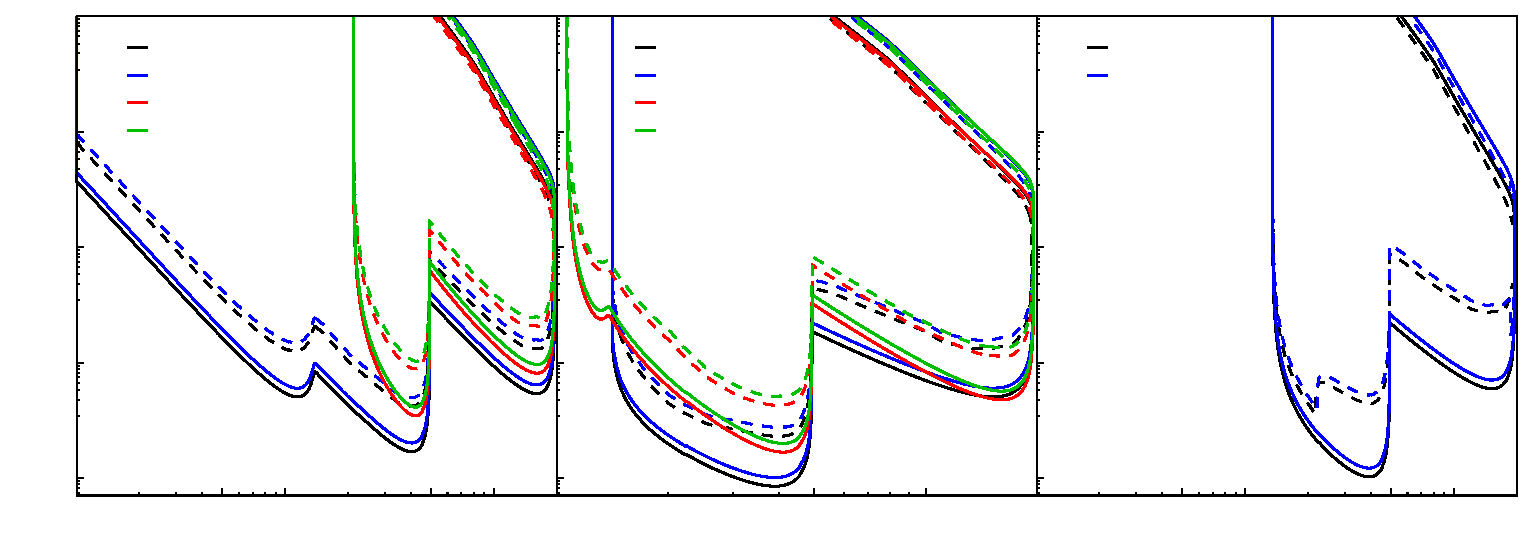
\includegraphics{pics/sensmulti_EW2_real}}%
    \gplfronttext
  \end{picture}%
\endgroup
}}
	\vspace{0.05em}

	%{\resizebox{\linewidth}{!}{\input{pics/sensmulti_MW.tex}}}
	{\resizebox{\linewidth}{!}{% GNUPLOT: LaTeX picture with Postscript
\begingroup
  \makeatletter
  \providecommand\color[2][]{%
    \GenericError{(gnuplot) \space\space\space\@spaces}{%
      Package color not loaded in conjunction with
      terminal option `colourtext'%
    }{See the gnuplot documentation for explanation.%
    }{Either use 'blacktext' in gnuplot or load the package
      color.sty in LaTeX.}%
    \renewcommand\color[2][]{}%
  }%
  \providecommand\includegraphics[2][]{%
    \GenericError{(gnuplot) \space\space\space\@spaces}{%
      Package graphicx or graphics not loaded%
    }{See the gnuplot documentation for explanation.%
    }{The gnuplot epslatex terminal needs graphicx.sty or graphics.sty.}%
    \renewcommand\includegraphics[2][]{}%
  }%
  \providecommand\rotatebox[2]{#2}%
  \@ifundefined{ifGPcolor}{%
    \newif\ifGPcolor
    \GPcolortrue
  }{}%
  \@ifundefined{ifGPblacktext}{%
    \newif\ifGPblacktext
    \GPblacktexttrue
  }{}%
  % define a \g@addto@macro without @ in the name:
  \let\gplgaddtomacro\g@addto@macro
  % define empty templates for all commands taking text:
  \gdef\gplbacktext{}%
  \gdef\gplfronttext{}%
  \makeatother
  \ifGPblacktext
    % no textcolor at all
    \def\colorrgb#1{}%
    \def\colorgray#1{}%
  \else
    % gray or color?
    \ifGPcolor
      \def\colorrgb#1{\color[rgb]{#1}}%
      \def\colorgray#1{\color[gray]{#1}}%
      \expandafter\def\csname LTw\endcsname{\color{white}}%
      \expandafter\def\csname LTb\endcsname{\color{black}}%
      \expandafter\def\csname LTa\endcsname{\color{black}}%
      \expandafter\def\csname LT0\endcsname{\color[rgb]{1,0,0}}%
      \expandafter\def\csname LT1\endcsname{\color[rgb]{0,1,0}}%
      \expandafter\def\csname LT2\endcsname{\color[rgb]{0,0,1}}%
      \expandafter\def\csname LT3\endcsname{\color[rgb]{1,0,1}}%
      \expandafter\def\csname LT4\endcsname{\color[rgb]{0,1,1}}%
      \expandafter\def\csname LT5\endcsname{\color[rgb]{1,1,0}}%
      \expandafter\def\csname LT6\endcsname{\color[rgb]{0,0,0}}%
      \expandafter\def\csname LT7\endcsname{\color[rgb]{1,0.3,0}}%
      \expandafter\def\csname LT8\endcsname{\color[rgb]{0.5,0.5,0.5}}%
    \else
      % gray
      \def\colorrgb#1{\color{black}}%
      \def\colorgray#1{\color[gray]{#1}}%
      \expandafter\def\csname LTw\endcsname{\color{white}}%
      \expandafter\def\csname LTb\endcsname{\color{black}}%
      \expandafter\def\csname LTa\endcsname{\color{black}}%
      \expandafter\def\csname LT0\endcsname{\color{black}}%
      \expandafter\def\csname LT1\endcsname{\color{black}}%
      \expandafter\def\csname LT2\endcsname{\color{black}}%
      \expandafter\def\csname LT3\endcsname{\color{black}}%
      \expandafter\def\csname LT4\endcsname{\color{black}}%
      \expandafter\def\csname LT5\endcsname{\color{black}}%
      \expandafter\def\csname LT6\endcsname{\color{black}}%
      \expandafter\def\csname LT7\endcsname{\color{black}}%
      \expandafter\def\csname LT8\endcsname{\color{black}}%
    \fi
  \fi
    \setlength{\unitlength}{0.0500bp}%
    \ifx\gptboxheight\undefined%
      \newlength{\gptboxheight}%
      \newlength{\gptboxwidth}%
      \newsavebox{\gptboxtext}%
    \fi%
    \setlength{\fboxrule}{0.5pt}%
    \setlength{\fboxsep}{1pt}%
\begin{picture}(14400.00,5040.00)%
    \gplgaddtomacro\gplbacktext{%
      \csname LTb\endcsname%%
      \put(444,607){\makebox(0,0)[r]{\strut{}\np{e-10}}}%
      \put(444,1715){\makebox(0,0)[r]{\strut{}\np{e-8}}}%
      \put(444,2823){\makebox(0,0)[r]{\strut{}\np{e-6}}}%
      \put(444,3931){\makebox(0,0)[r]{\strut{}\np{e-4}}}%
      \put(444,5039){\makebox(0,0)[r]{\strut{}\np{e-2}}}%
      \put(1975,220){\makebox(0,0){\strut{}$0.05$}}%
      \put(3978,220){\makebox(0,0){\strut{}$0.5$}}%
      \put(576,220){\makebox(0,0){\strut{}$0.01$}}%
      \put(2578,220){\makebox(0,0){\strut{}$0.1$}}%
      \put(4580,220){\makebox(0,0){\strut{}$1$}}%
    }%
    \gplgaddtomacro\gplfronttext{%
      \csname LTb\endcsname%%
      \put(-436,2739){\rotatebox{-270}{\makebox(0,0){\strut{}$ |U_{\mu N}|^2 $}}}%
      \put(2879,-110){\makebox(0,0){\strut{}Mass (GeV)}}%
      \csname LTb\endcsname%%
      \put(1388,1583){\makebox(0,0)[l]{\strut{}$\nu e e $ Majorana}}%
      \csname LTb\endcsname%%
      \put(1388,1319){\makebox(0,0)[l]{\strut{}$\nu e e $ Dirac}}%
      \csname LTb\endcsname%%
      \put(1388,1055){\makebox(0,0)[l]{\strut{}$\nu \mu \mu $ Majorana}}%
      \csname LTb\endcsname%%
      \put(1388,791){\makebox(0,0)[l]{\strut{}$\nu \mu \mu $ Dirac}}%
    }%
    \gplgaddtomacro\gplbacktext{%
      \csname LTb\endcsname%%
      \put(5052,607){\makebox(0,0)[r]{\strut{}}}%
      \put(5052,1715){\makebox(0,0)[r]{\strut{}}}%
      \put(5052,2823){\makebox(0,0)[r]{\strut{}}}%
      \put(5052,3931){\makebox(0,0)[r]{\strut{}}}%
      \put(5052,5039){\makebox(0,0)[r]{\strut{}}}%
      \put(7659,220){\makebox(0,0){\strut{}$0.5$}}%
      \put(5184,220){\makebox(0,0){\strut{}$0.1$}}%
      \put(8725,220){\makebox(0,0){\strut{}$1$}}%
    }%
    \gplgaddtomacro\gplfronttext{%
      \csname LTb\endcsname%%
      \put(7487,-110){\makebox(0,0){\strut{}Mass (GeV)}}%
      \csname LTb\endcsname%%
      \put(8118,1583){\makebox(0,0)[l]{\strut{}$\mu \pi $ Majorana}}%
      \csname LTb\endcsname%%
      \put(8118,1319){\makebox(0,0)[l]{\strut{}$\mu \pi $ Dirac}}%
      \csname LTb\endcsname%%
      \put(8118,1055){\makebox(0,0)[l]{\strut{}$\nu e \mu $ Majorana}}%
      \csname LTb\endcsname%%
      \put(8118,791){\makebox(0,0)[l]{\strut{}$\nu e \mu $ Dirac}}%
    }%
    \gplgaddtomacro\gplbacktext{%
      \csname LTb\endcsname%%
      \put(9660,607){\makebox(0,0)[r]{\strut{}}}%
      \put(9660,1715){\makebox(0,0)[r]{\strut{}}}%
      \put(9660,2823){\makebox(0,0)[r]{\strut{}}}%
      \put(9660,3931){\makebox(0,0)[r]{\strut{}}}%
      \put(9660,5039){\makebox(0,0)[r]{\strut{}}}%
      \put(11191,220){\makebox(0,0){\strut{}$0.05$}}%
      \put(13194,220){\makebox(0,0){\strut{}$0.5$}}%
      \put(14399,220){\makebox(0,0){\strut{}$2$}}%
      \put(9792,220){\makebox(0,0){\strut{}$0.01$}}%
      \put(11794,220){\makebox(0,0){\strut{}$0.1$}}%
      \put(13796,220){\makebox(0,0){\strut{}$1$}}%
    }%
    \gplgaddtomacro\gplfronttext{%
      \csname LTb\endcsname%%
      \put(12095,-110){\makebox(0,0){\strut{}Mass (GeV)}}%
      \csname LTb\endcsname%%
      \put(10604,1583){\makebox(0,0)[l]{\strut{}$\nu \pi^0 $ Majorana}}%
      \csname LTb\endcsname%%
      \put(10604,1319){\makebox(0,0)[l]{\strut{}$\nu \pi^0 $ Dirac}}%
    }%
    \gplbacktext
    \put(0,0){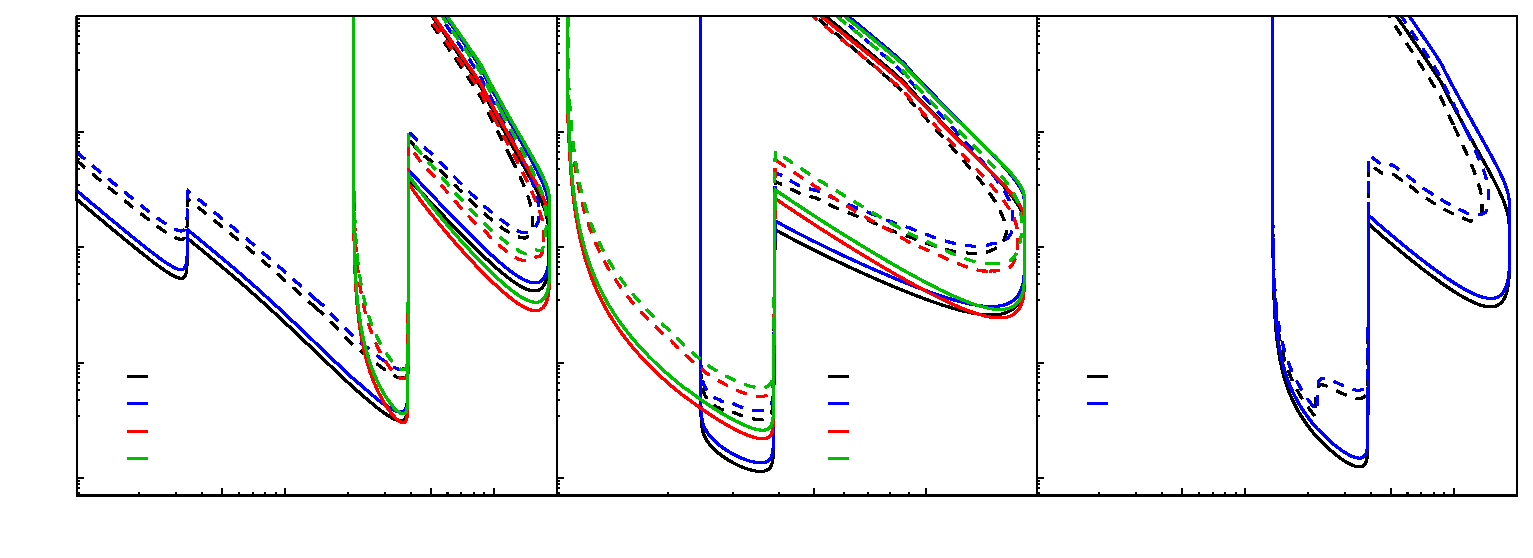
\includegraphics{pics/sensmulti_MW2_real}}%
    \gplfronttext
  \end{picture}%
\endgroup
}}
	\vspace{0.05em}

	%{\resizebox{\linewidth}{!}{\input{pics/sensmulti_TW.tex}}}
	{\resizebox{\linewidth}{!}{% GNUPLOT: LaTeX picture with Postscript
\begingroup
  \makeatletter
  \providecommand\color[2][]{%
    \GenericError{(gnuplot) \space\space\space\@spaces}{%
      Package color not loaded in conjunction with
      terminal option `colourtext'%
    }{See the gnuplot documentation for explanation.%
    }{Either use 'blacktext' in gnuplot or load the package
      color.sty in LaTeX.}%
    \renewcommand\color[2][]{}%
  }%
  \providecommand\includegraphics[2][]{%
    \GenericError{(gnuplot) \space\space\space\@spaces}{%
      Package graphicx or graphics not loaded%
    }{See the gnuplot documentation for explanation.%
    }{The gnuplot epslatex terminal needs graphicx.sty or graphics.sty.}%
    \renewcommand\includegraphics[2][]{}%
  }%
  \providecommand\rotatebox[2]{#2}%
  \@ifundefined{ifGPcolor}{%
    \newif\ifGPcolor
    \GPcolortrue
  }{}%
  \@ifundefined{ifGPblacktext}{%
    \newif\ifGPblacktext
    \GPblacktexttrue
  }{}%
  % define a \g@addto@macro without @ in the name:
  \let\gplgaddtomacro\g@addto@macro
  % define empty templates for all commands taking text:
  \gdef\gplbacktext{}%
  \gdef\gplfronttext{}%
  \makeatother
  \ifGPblacktext
    % no textcolor at all
    \def\colorrgb#1{}%
    \def\colorgray#1{}%
  \else
    % gray or color?
    \ifGPcolor
      \def\colorrgb#1{\color[rgb]{#1}}%
      \def\colorgray#1{\color[gray]{#1}}%
      \expandafter\def\csname LTw\endcsname{\color{white}}%
      \expandafter\def\csname LTb\endcsname{\color{black}}%
      \expandafter\def\csname LTa\endcsname{\color{black}}%
      \expandafter\def\csname LT0\endcsname{\color[rgb]{1,0,0}}%
      \expandafter\def\csname LT1\endcsname{\color[rgb]{0,1,0}}%
      \expandafter\def\csname LT2\endcsname{\color[rgb]{0,0,1}}%
      \expandafter\def\csname LT3\endcsname{\color[rgb]{1,0,1}}%
      \expandafter\def\csname LT4\endcsname{\color[rgb]{0,1,1}}%
      \expandafter\def\csname LT5\endcsname{\color[rgb]{1,1,0}}%
      \expandafter\def\csname LT6\endcsname{\color[rgb]{0,0,0}}%
      \expandafter\def\csname LT7\endcsname{\color[rgb]{1,0.3,0}}%
      \expandafter\def\csname LT8\endcsname{\color[rgb]{0.5,0.5,0.5}}%
    \else
      % gray
      \def\colorrgb#1{\color{black}}%
      \def\colorgray#1{\color[gray]{#1}}%
      \expandafter\def\csname LTw\endcsname{\color{white}}%
      \expandafter\def\csname LTb\endcsname{\color{black}}%
      \expandafter\def\csname LTa\endcsname{\color{black}}%
      \expandafter\def\csname LT0\endcsname{\color{black}}%
      \expandafter\def\csname LT1\endcsname{\color{black}}%
      \expandafter\def\csname LT2\endcsname{\color{black}}%
      \expandafter\def\csname LT3\endcsname{\color{black}}%
      \expandafter\def\csname LT4\endcsname{\color{black}}%
      \expandafter\def\csname LT5\endcsname{\color{black}}%
      \expandafter\def\csname LT6\endcsname{\color{black}}%
      \expandafter\def\csname LT7\endcsname{\color{black}}%
      \expandafter\def\csname LT8\endcsname{\color{black}}%
    \fi
  \fi
    \setlength{\unitlength}{0.0500bp}%
    \ifx\gptboxheight\undefined%
      \newlength{\gptboxheight}%
      \newlength{\gptboxwidth}%
      \newsavebox{\gptboxtext}%
    \fi%
    \setlength{\fboxrule}{0.5pt}%
    \setlength{\fboxsep}{1pt}%
\begin{picture}(14400.00,5040.00)%
    \gplgaddtomacro\gplbacktext{%
      \csname LTb\endcsname%%
      \put(2748,1097){\makebox(0,0)[r]{\strut{}\np{e-6}}}%
      \put(2748,2411){\makebox(0,0)[r]{\strut{}\np{e-4}}}%
      \put(2748,3725){\makebox(0,0)[r]{\strut{}\np{e-2}}}%
      \put(2748,5039){\makebox(0,0)[r]{\strut{}\np{1}}}%
      \put(4279,220){\makebox(0,0){\strut{}$0.05$}}%
      \put(6282,220){\makebox(0,0){\strut{}$0.5$}}%
      \put(2880,220){\makebox(0,0){\strut{}$0.01$}}%
      \put(4882,220){\makebox(0,0){\strut{}$0.1$}}%
      \put(6884,220){\makebox(0,0){\strut{}$1$}}%
    }%
    \gplgaddtomacro\gplfronttext{%
      \csname LTb\endcsname%%
      \put(2000,2739){\rotatebox{-270}{\makebox(0,0){\strut{}$ |U_{\tau N}|^2 $}}}%
      \put(5183,-110){\makebox(0,0){\strut{}Mass (GeV)}}%
      \csname LTb\endcsname%%
      \put(3692,2081){\makebox(0,0)[l]{\strut{}$\nu e e $ Majorana}}%
      \csname LTb\endcsname%%
      \put(3692,1817){\makebox(0,0)[l]{\strut{}$\nu e e $ Dirac}}%
      \csname LTb\endcsname%%
      \put(3692,1553){\makebox(0,0)[l]{\strut{}$\nu \mu \mu $ Majorana}}%
      \csname LTb\endcsname%%
      \put(3692,1289){\makebox(0,0)[l]{\strut{}$\nu \mu \mu $ Dirac}}%
    }%
    \gplgaddtomacro\gplbacktext{%
      \csname LTb\endcsname%%
      \put(7355,1097){\makebox(0,0)[r]{\strut{}}}%
      \put(7355,2411){\makebox(0,0)[r]{\strut{}}}%
      \put(7355,3725){\makebox(0,0)[r]{\strut{}}}%
      \put(7355,5039){\makebox(0,0)[r]{\strut{}}}%
      \put(8887,220){\makebox(0,0){\strut{}$0.05$}}%
      \put(10889,220){\makebox(0,0){\strut{}$0.5$}}%
      \put(12095,220){\makebox(0,0){\strut{}$2$}}%
      \put(7487,220){\makebox(0,0){\strut{}$0.01$}}%
      \put(9490,220){\makebox(0,0){\strut{}$0.1$}}%
      \put(11492,220){\makebox(0,0){\strut{}$1$}}%
    }%
    \gplgaddtomacro\gplfronttext{%
      \csname LTb\endcsname%%
      \put(9791,-110){\makebox(0,0){\strut{}Mass (GeV)}}%
      \csname LTb\endcsname%%
      \put(8299,2081){\makebox(0,0)[l]{\strut{}$\nu \pi^0 $ Majorana}}%
      \csname LTb\endcsname%%
      \put(8299,1817){\makebox(0,0)[l]{\strut{}$\nu \pi^0 $ Dirac}}%
    }%
    \gplbacktext
    \put(0,0){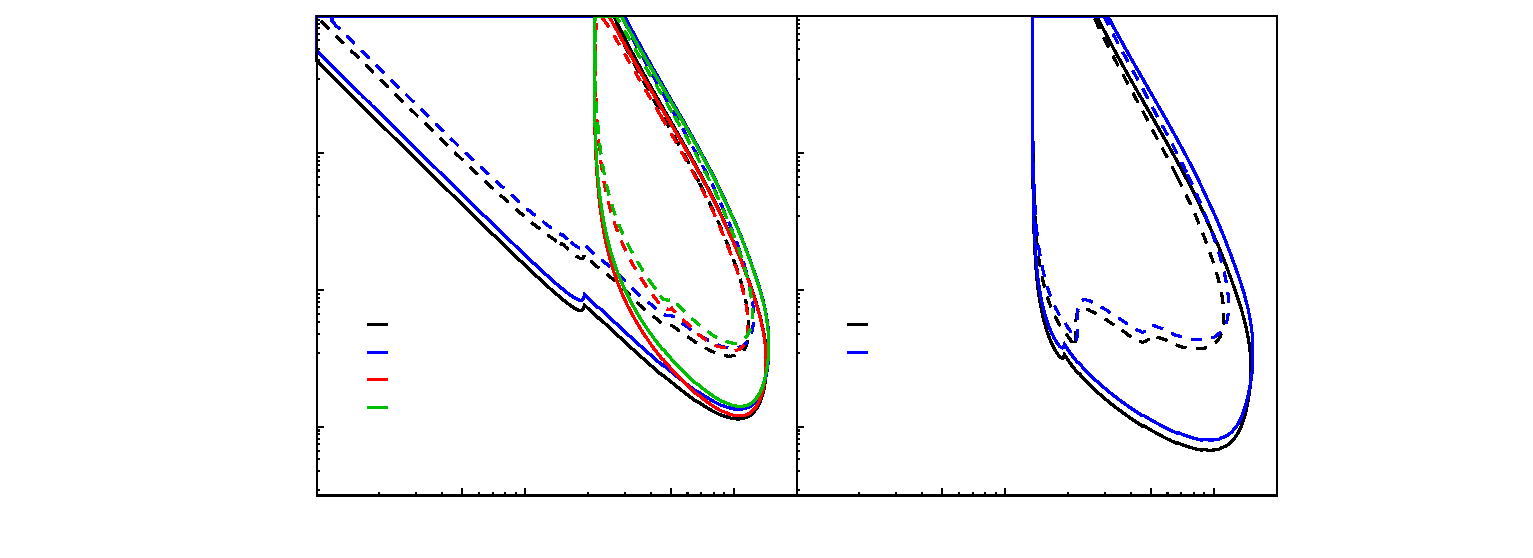
\includegraphics{pics/sensmulti_TW2_real}}%
    \gplfronttext
  \end{picture}%
\endgroup
}}

	\caption{The 90\,\% C.L. sensitivity regions to individual channels for dominant mixings %
		$|U_{e N}|^2$ (top), $|U_{\mu N}|^2$ (middle), and $|U_{\tau N}|^2$ (bottom) are shown.
		The solid lines correspond to the analysis before the background analysis, which is equivalent %
		to a weighting factor $W_d = 1$ (see~\refeq{eq:event}).
		The dashed lines are drawn after our background analysis.
		The distinction between the fermionic natures are explained in the colour key.}
	\label{fig:senseW}
\end{figure}

In this section, we present the sensitivity regions for the three mixings $|U_{e N}|^2$, $|U_{\mu N}|^2$, and %
$|U_{\tau N}|^2$, where we assume that just one mixing element dominates over the other two.
The~sensitivities for the decay channels $N\to\nu e^+ e^-$, $\nu e^\pm \mu^\mp$, $\nu \mu^+ \mu^-$, $\nu \pi^0$, % 
$e^\mp \pi^\pm$ ($|U_{e N}|^2$ only), and $\mu^\mp \pi^\pm$ ($|U_{\mu N}|^2$ only) are reported in \reffig{fig:senseW}.
The solid lines corresponds to a scenario in which zero background is assumed at the ND.
%The introduction of background worsens the sensitives, the lines of which are represented by dashed lines.
A background study is done for these channels (see~\refsec{sec:background}), to outline a more realistic sensitivity; %
the resulting regions are shown as dashed lines in \reffig{fig:senseW}.
As we expect that further improvements to background reduction can be achieved %
with a dedicated analysis by the experimental collaboration, %
the final sensitivity will lie somewhere between the lines with and without backgrounds.

For both the electronic and the muonic mixings, the two-body semi-leptonic decay modes are the ones providing %
the best sensitivity for sufficiently heavy masses.
With the channel $N\to e^\mp \pi^\pm$, the mixing can be constrained in the range %
$0.15\,\text{GeV} \lesssim m_N \lesssim 0.49\,\text{GeV}$ %
to be $|U_{e N}|^2 < \np{3e-9}$, with a minimum point $|U_{e N}|^2 < \np{7e-11}$ at $m_N \simeq 0.39$\,GeV.
Including the background rejection, the limits are loosened by a factor of $\sim$6.1.
The~channel $N\to \mu^\mp \pi^\pm$ can constrain the mixing $|U_{\mu N}|^2 < \np{5.6e-10}$ %
in the mass range \mbox{$0.25\,\text{GeV} \lesssim m_N \lesssim 0.39\,\text{GeV}$}, %
with the best limit $|U_{\mu N}|^2 < \np{1.3e-10}$ at $m_N \simeq 0.35$\,GeV.
In this case, the higher background reduce the bounds up to a factor of $\sim$14.3.
The NC decay $N\to \nu \pi^0$ is the channel most affected by background and with the worst signal efficiency: %
the limits are higher at most by a factor of~$\sim$29.6 for the electronic, %
$\sim$36.5 for the muonic, and~$\sim$42.5 for the tau mixing.
Assuming no background, instead, the constrains placed by this decay mode can be competitive, as the %
mixings are limited to be $|U_{e N}|^2 < \np{1.1e-10}$ at $m_N \simeq 0.39$\,GeV, %
$|U_{\mu N}|^2 < \np{1.5e-10}$ at $m_N \simeq 0.35$\,GeV, %
and $|U_{\tau N}|^2 < \np{6.70e-7}$ at $m_N \simeq 0.95$\,GeV.
%This difference is due to the fact that charge-ID is not taken in account in our analysis.
There is no sensitivity to the channel $N\to\tau^\mp\pi^\pm$ because of the subdominant branching ratio %
and flux content.

The three-body lepton decays have a lower reach, but are more sensitive to masses above the kaon mass limit %
than the two-body semi-leptonic modes.
The channel $N\to \nu e^- e^+$ is the only one that covers the whole mass range of interest %
and the bounds are weakened by background reduction by a factor less than 6.
It can limit the electronic mixing down to $|U_{e N}|^2 < \np{2.5e-9}$ at $m_N \simeq 0.11$\,GeV, %
$|U_{e N}|^2 < \np{2.9e-10}$ at $m_N \simeq 0.39$\,GeV, and $|U_{e N}|^2 < \np{3.0e-9}$ at $m_N \simeq 1.6$\,GeV.
The channels $N \to\nu \mu^- \mu^+$ and $\nu e^\pm \mu^\mp$ perform better with the muon mixing, %
despite suffering more from background rejection, up to a factor of 16 for the muon mixing and a factor of 17 %
for the tau mixing.
They respectively give the limits %
$|U_{\mu N}|^2 < \np{9.0e-10}$ at $m_N \simeq 0.37$\,GeV and $|U_{\mu N}|^2 < \np{8.2e-8}$ at $m_N \simeq 1.6$\,GeV, and %
$|U_{\mu N}|^2 < \np{4.7e-10}$ at $m_N \simeq 0.36$\,GeV and $|U_{\mu N}|^2 < \np{6.1e-8}$ at $m_N \simeq 1.6$\,GeV.
The $\tau$ sector can only be constrained by the two NC--mediated channels, %
which give very similar constraints near $m_N\simeq 1.0$\,GeV, these being $|U_{\tau N}|^2 < \np{2.2e-6}$ 
for the $\nu e^- e^+$ channel and $|U_{\tau N}|^2 < \np{2.2e-6}$ for the $\nu \mu^- \mu ^+$ channel.

%These regions are naturally weakened when the background analysis is taken in account.
%Instead of performing an event simulation for each value of the heavy neutrino mass, %
%we study the background expectancy only for 9 equally-spaced choices of heavy neutrino mass from 50 MeV to 450 MeV and we interpolate in between.
%%
%	%The weighting factors $W_d$ explained in section~\ref{sec:numevt} are extrapolated in the same manner.
%The channels less afflicted from background reduction analysis are the decays $N\to \ell_\alpha^- \pi^+$, %
%$N\to \nu e^-e^+$, and $N\to \nu e^\mp\mu^\pm$, the sensitivities of which are reduced by less than a factor of 10.
%The other channels present more background and the reduction in the sensitivity is slightly more than one order of magnitude.
%No background analysis is made for masses above the kaon mass.

\begin{figure}
	\centering
	%{\resizebox{\linewidth}{!}{\input{pics/sens_EM_V.tex}}}
	{\resizebox{\linewidth}{!}{% GNUPLOT: LaTeX picture with Postscript
\begingroup
  \makeatletter
  \providecommand\color[2][]{%
    \GenericError{(gnuplot) \space\space\space\@spaces}{%
      Package color not loaded in conjunction with
      terminal option `colourtext'%
    }{See the gnuplot documentation for explanation.%
    }{Either use 'blacktext' in gnuplot or load the package
      color.sty in LaTeX.}%
    \renewcommand\color[2][]{}%
  }%
  \providecommand\includegraphics[2][]{%
    \GenericError{(gnuplot) \space\space\space\@spaces}{%
      Package graphicx or graphics not loaded%
    }{See the gnuplot documentation for explanation.%
    }{The gnuplot epslatex terminal needs graphicx.sty or graphics.sty.}%
    \renewcommand\includegraphics[2][]{}%
  }%
  \providecommand\rotatebox[2]{#2}%
  \@ifundefined{ifGPcolor}{%
    \newif\ifGPcolor
    \GPcolortrue
  }{}%
  \@ifundefined{ifGPblacktext}{%
    \newif\ifGPblacktext
    \GPblacktexttrue
  }{}%
  % define a \g@addto@macro without @ in the name:
  \let\gplgaddtomacro\g@addto@macro
  % define empty templates for all commands taking text:
  \gdef\gplbacktext{}%
  \gdef\gplfronttext{}%
  \makeatother
  \ifGPblacktext
    % no textcolor at all
    \def\colorrgb#1{}%
    \def\colorgray#1{}%
  \else
    % gray or color?
    \ifGPcolor
      \def\colorrgb#1{\color[rgb]{#1}}%
      \def\colorgray#1{\color[gray]{#1}}%
      \expandafter\def\csname LTw\endcsname{\color{white}}%
      \expandafter\def\csname LTb\endcsname{\color{black}}%
      \expandafter\def\csname LTa\endcsname{\color{black}}%
      \expandafter\def\csname LT0\endcsname{\color[rgb]{1,0,0}}%
      \expandafter\def\csname LT1\endcsname{\color[rgb]{0,1,0}}%
      \expandafter\def\csname LT2\endcsname{\color[rgb]{0,0,1}}%
      \expandafter\def\csname LT3\endcsname{\color[rgb]{1,0,1}}%
      \expandafter\def\csname LT4\endcsname{\color[rgb]{0,1,1}}%
      \expandafter\def\csname LT5\endcsname{\color[rgb]{1,1,0}}%
      \expandafter\def\csname LT6\endcsname{\color[rgb]{0,0,0}}%
      \expandafter\def\csname LT7\endcsname{\color[rgb]{1,0.3,0}}%
      \expandafter\def\csname LT8\endcsname{\color[rgb]{0.5,0.5,0.5}}%
    \else
      % gray
      \def\colorrgb#1{\color{black}}%
      \def\colorgray#1{\color[gray]{#1}}%
      \expandafter\def\csname LTw\endcsname{\color{white}}%
      \expandafter\def\csname LTb\endcsname{\color{black}}%
      \expandafter\def\csname LTa\endcsname{\color{black}}%
      \expandafter\def\csname LT0\endcsname{\color{black}}%
      \expandafter\def\csname LT1\endcsname{\color{black}}%
      \expandafter\def\csname LT2\endcsname{\color{black}}%
      \expandafter\def\csname LT3\endcsname{\color{black}}%
      \expandafter\def\csname LT4\endcsname{\color{black}}%
      \expandafter\def\csname LT5\endcsname{\color{black}}%
      \expandafter\def\csname LT6\endcsname{\color{black}}%
      \expandafter\def\csname LT7\endcsname{\color{black}}%
      \expandafter\def\csname LT8\endcsname{\color{black}}%
    \fi
  \fi
    \setlength{\unitlength}{0.0500bp}%
    \ifx\gptboxheight\undefined%
      \newlength{\gptboxheight}%
      \newlength{\gptboxwidth}%
      \newsavebox{\gptboxtext}%
    \fi%
    \setlength{\fboxrule}{0.5pt}%
    \setlength{\fboxsep}{1pt}%
\begin{picture}(14400.00,5040.00)%
    \gplgaddtomacro\gplbacktext{%
      \csname LTb\endcsname%%
      \put(444,951){\makebox(0,0)[r]{\strut{}\np{e-8}}}%
      \put(444,1973){\makebox(0,0)[r]{\strut{}\np{e-6}}}%
      \put(444,2995){\makebox(0,0)[r]{\strut{}\np{e-4}}}%
      \put(444,4017){\makebox(0,0)[r]{\strut{}\np{e-2}}}%
      \put(444,5039){\makebox(0,0)[r]{\strut{}\np{e0}}}%
      \put(1015,220){\makebox(0,0){\strut{}$0.5$}}%
      \put(2379,220){\makebox(0,0){\strut{}$1$}}%
    }%
    \gplgaddtomacro\gplfronttext{%
      \csname LTb\endcsname%%
      \put(-304,2739){\rotatebox{-270}{\makebox(0,0){\strut{}$ |U_{e N}|^2 $}}}%
      \put(2159,-110){\makebox(0,0){\strut{}Mass (GeV)}}%
      \csname LTb\endcsname%%
      \put(2838,4753){\makebox(0,0)[l]{\strut{}$e K$}}%
      \csname LTb\endcsname%%
      \put(2838,4489){\makebox(0,0)[l]{\strut{}$e K^*$}}%
      \csname LTb\endcsname%%
      \put(2838,4225){\makebox(0,0)[l]{\strut{}$e \rho$}}%
      \csname LTb\endcsname%%
      \put(2838,3961){\makebox(0,0)[l]{\strut{}$\nu\rho^0$}}%
    }%
    \gplgaddtomacro\gplbacktext{%
      \csname LTb\endcsname%%
      \put(3611,951){\makebox(0,0)[r]{\strut{}}}%
      \put(3611,1973){\makebox(0,0)[r]{\strut{}}}%
      \put(3611,2995){\makebox(0,0)[r]{\strut{}}}%
      \put(3611,4017){\makebox(0,0)[r]{\strut{}}}%
      \put(3611,5039){\makebox(0,0)[r]{\strut{}}}%
      \put(4182,220){\makebox(0,0){\strut{}$0.5$}}%
      \put(6911,220){\makebox(0,0){\strut{}$2$}}%
      \put(5547,220){\makebox(0,0){\strut{}$1$}}%
    }%
    \gplgaddtomacro\gplfronttext{%
      \csname LTb\endcsname%%
      \put(5327,-110){\makebox(0,0){\strut{}Mass (GeV)}}%
      \csname LTb\endcsname%%
      \put(6006,4753){\makebox(0,0)[l]{\strut{}$\nu\eta$}}%
      \csname LTb\endcsname%%
      \put(6006,4489){\makebox(0,0)[l]{\strut{}$\nu\eta'$}}%
      \csname LTb\endcsname%%
      \put(6006,4225){\makebox(0,0)[l]{\strut{}$\nu\omega$}}%
      \csname LTb\endcsname%%
      \put(6006,3961){\makebox(0,0)[l]{\strut{}$\nu\phi$}}%
    }%
    \gplgaddtomacro\gplbacktext{%
      \csname LTb\endcsname%%
      \put(7932,951){\makebox(0,0)[r]{\strut{}\np{e-8}}}%
      \put(7932,1973){\makebox(0,0)[r]{\strut{}\np{e-6}}}%
      \put(7932,2995){\makebox(0,0)[r]{\strut{}\np{e-4}}}%
      \put(7932,4017){\makebox(0,0)[r]{\strut{}\np{e-2}}}%
      \put(7932,5039){\makebox(0,0)[r]{\strut{}\np{e0}}}%
      \put(8064,220){\makebox(0,0){\strut{}$0.5$}}%
      \put(9648,220){\makebox(0,0){\strut{}$1$}}%
    }%
    \gplgaddtomacro\gplfronttext{%
      \csname LTb\endcsname%%
      \put(7184,2739){\rotatebox{-270}{\makebox(0,0){\strut{}$ |U_{\mu 4}|^2 $}}}%
      \put(9647,-110){\makebox(0,0){\strut{}Mass (GeV)}}%
      \csname LTb\endcsname%%
      \put(10107,4753){\makebox(0,0)[l]{\strut{}$\mu K$}}%
      \csname LTb\endcsname%%
      \put(10107,4489){\makebox(0,0)[l]{\strut{}$\mu K^*$}}%
      \csname LTb\endcsname%%
      \put(10107,4225){\makebox(0,0)[l]{\strut{}$\mu \rho$}}%
      \csname LTb\endcsname%%
      \put(10107,3961){\makebox(0,0)[l]{\strut{}$\nu \rho^0$}}%
    }%
    \gplgaddtomacro\gplbacktext{%
      \csname LTb\endcsname%%
      \put(11100,951){\makebox(0,0)[r]{\strut{}}}%
      \put(11100,1973){\makebox(0,0)[r]{\strut{}}}%
      \put(11100,2995){\makebox(0,0)[r]{\strut{}}}%
      \put(11100,4017){\makebox(0,0)[r]{\strut{}}}%
      \put(11100,5039){\makebox(0,0)[r]{\strut{}}}%
      \put(11232,220){\makebox(0,0){\strut{}$0.5$}}%
      \put(14399,220){\makebox(0,0){\strut{}$2$}}%
      \put(12816,220){\makebox(0,0){\strut{}$1$}}%
    }%
    \gplgaddtomacro\gplfronttext{%
      \csname LTb\endcsname%%
      \put(12815,-110){\makebox(0,0){\strut{}Mass (GeV)}}%
      \csname LTb\endcsname%%
      \put(13275,4753){\makebox(0,0)[l]{\strut{}$\nu\eta$}}%
      \csname LTb\endcsname%%
      \put(13275,4489){\makebox(0,0)[l]{\strut{}$\nu\eta'$}}%
      \csname LTb\endcsname%%
      \put(13275,4225){\makebox(0,0)[l]{\strut{}$\nu\omega$}}%
      \csname LTb\endcsname%%
      \put(13275,3961){\makebox(0,0)[l]{\strut{}$\nu\phi$}}%
    }%
    \gplbacktext
    \put(0,0){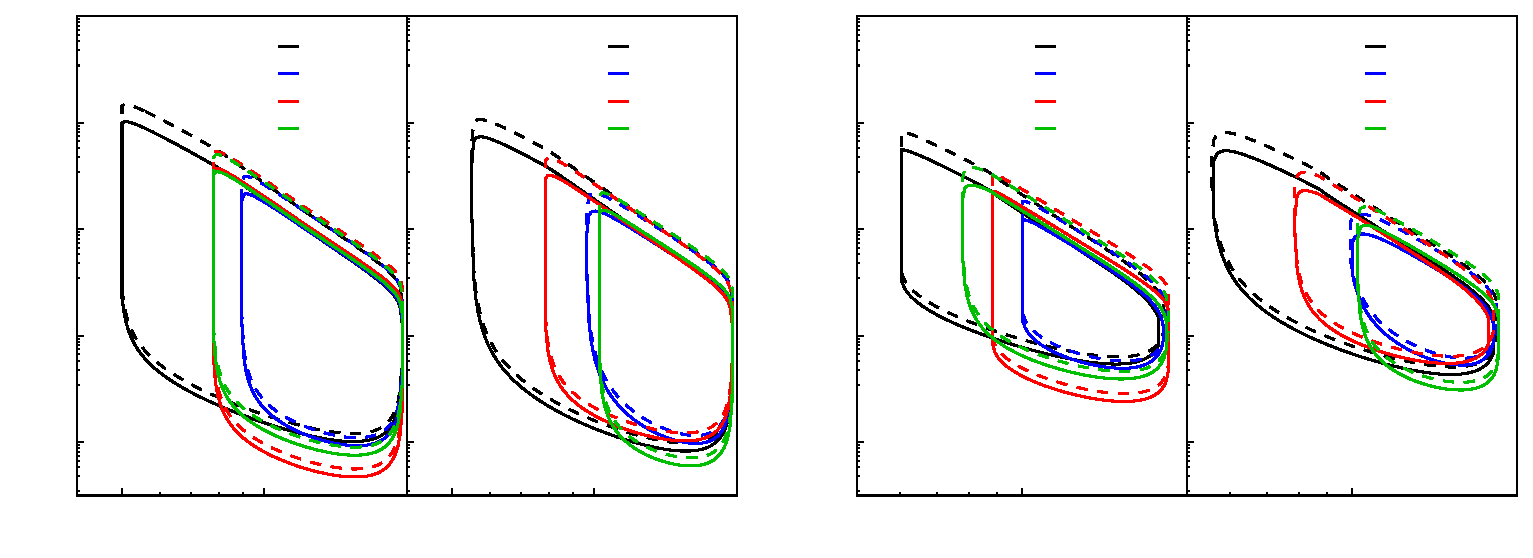
\includegraphics{pics/sensmulti_EM_V2_real}}%
    \gplfronttext
  \end{picture}%
\endgroup
}}
	\vspace{0.05em}

	%{\resizebox{\linewidth}{!}{\input{pics/sens_T_V.tex}}}
	{\resizebox{\linewidth}{!}{% GNUPLOT: LaTeX picture with Postscript
\begingroup
  \makeatletter
  \providecommand\color[2][]{%
    \GenericError{(gnuplot) \space\space\space\@spaces}{%
      Package color not loaded in conjunction with
      terminal option `colourtext'%
    }{See the gnuplot documentation for explanation.%
    }{Either use 'blacktext' in gnuplot or load the package
      color.sty in LaTeX.}%
    \renewcommand\color[2][]{}%
  }%
  \providecommand\includegraphics[2][]{%
    \GenericError{(gnuplot) \space\space\space\@spaces}{%
      Package graphicx or graphics not loaded%
    }{See the gnuplot documentation for explanation.%
    }{The gnuplot epslatex terminal needs graphicx.sty or graphics.sty.}%
    \renewcommand\includegraphics[2][]{}%
  }%
  \providecommand\rotatebox[2]{#2}%
  \@ifundefined{ifGPcolor}{%
    \newif\ifGPcolor
    \GPcolortrue
  }{}%
  \@ifundefined{ifGPblacktext}{%
    \newif\ifGPblacktext
    \GPblacktexttrue
  }{}%
  % define a \g@addto@macro without @ in the name:
  \let\gplgaddtomacro\g@addto@macro
  % define empty templates for all commands taking text:
  \gdef\gplbacktext{}%
  \gdef\gplfronttext{}%
  \makeatother
  \ifGPblacktext
    % no textcolor at all
    \def\colorrgb#1{}%
    \def\colorgray#1{}%
  \else
    % gray or color?
    \ifGPcolor
      \def\colorrgb#1{\color[rgb]{#1}}%
      \def\colorgray#1{\color[gray]{#1}}%
      \expandafter\def\csname LTw\endcsname{\color{white}}%
      \expandafter\def\csname LTb\endcsname{\color{black}}%
      \expandafter\def\csname LTa\endcsname{\color{black}}%
      \expandafter\def\csname LT0\endcsname{\color[rgb]{1,0,0}}%
      \expandafter\def\csname LT1\endcsname{\color[rgb]{0,1,0}}%
      \expandafter\def\csname LT2\endcsname{\color[rgb]{0,0,1}}%
      \expandafter\def\csname LT3\endcsname{\color[rgb]{1,0,1}}%
      \expandafter\def\csname LT4\endcsname{\color[rgb]{0,1,1}}%
      \expandafter\def\csname LT5\endcsname{\color[rgb]{1,1,0}}%
      \expandafter\def\csname LT6\endcsname{\color[rgb]{0,0,0}}%
      \expandafter\def\csname LT7\endcsname{\color[rgb]{1,0.3,0}}%
      \expandafter\def\csname LT8\endcsname{\color[rgb]{0.5,0.5,0.5}}%
    \else
      % gray
      \def\colorrgb#1{\color{black}}%
      \def\colorgray#1{\color[gray]{#1}}%
      \expandafter\def\csname LTw\endcsname{\color{white}}%
      \expandafter\def\csname LTb\endcsname{\color{black}}%
      \expandafter\def\csname LTa\endcsname{\color{black}}%
      \expandafter\def\csname LT0\endcsname{\color{black}}%
      \expandafter\def\csname LT1\endcsname{\color{black}}%
      \expandafter\def\csname LT2\endcsname{\color{black}}%
      \expandafter\def\csname LT3\endcsname{\color{black}}%
      \expandafter\def\csname LT4\endcsname{\color{black}}%
      \expandafter\def\csname LT5\endcsname{\color{black}}%
      \expandafter\def\csname LT6\endcsname{\color{black}}%
      \expandafter\def\csname LT7\endcsname{\color{black}}%
      \expandafter\def\csname LT8\endcsname{\color{black}}%
    \fi
  \fi
    \setlength{\unitlength}{0.0500bp}%
    \ifx\gptboxheight\undefined%
      \newlength{\gptboxheight}%
      \newlength{\gptboxwidth}%
      \newsavebox{\gptboxtext}%
    \fi%
    \setlength{\fboxrule}{0.5pt}%
    \setlength{\fboxsep}{1pt}%
\begin{picture}(14400.00,5040.00)%
    \gplgaddtomacro\gplbacktext{%
      \csname LTb\endcsname%%
      \put(4188,1097){\makebox(0,0)[r]{\strut{}\np{e-6}}}%
      \put(4188,2411){\makebox(0,0)[r]{\strut{}\np{e-4}}}%
      \put(4188,3725){\makebox(0,0)[r]{\strut{}\np{e-2}}}%
      \put(4188,5039){\makebox(0,0)[r]{\strut{}\np{1}}}%
      \put(4759,220){\makebox(0,0){\strut{}$0.5$}}%
      \put(6123,220){\makebox(0,0){\strut{}$1$}}%
    }%
    \gplgaddtomacro\gplfronttext{%
      \csname LTb\endcsname%%
      \put(3440,2739){\rotatebox{-270}{\makebox(0,0){\strut{}$ |U_{\tau N}|^2 $}}}%
      \put(5903,-110){\makebox(0,0){\strut{}Mass (GeV)}}%
      \csname LTb\endcsname%%
      \put(6582,4709){\makebox(0,0)[l]{\strut{}$\nu\eta$}}%
      \csname LTb\endcsname%%
      \put(6582,4445){\makebox(0,0)[l]{\strut{}$\nu\eta'$}}%
      \csname LTb\endcsname%%
      \put(6582,4181){\makebox(0,0)[l]{\strut{}$\nu\phi$}}%
    }%
    \gplgaddtomacro\gplbacktext{%
      \csname LTb\endcsname%%
      \put(7355,1097){\makebox(0,0)[r]{\strut{}}}%
      \put(7355,2411){\makebox(0,0)[r]{\strut{}}}%
      \put(7355,3725){\makebox(0,0)[r]{\strut{}}}%
      \put(7355,5039){\makebox(0,0)[r]{\strut{}}}%
      \put(7926,220){\makebox(0,0){\strut{}$0.5$}}%
      \put(10655,220){\makebox(0,0){\strut{}$2$}}%
      \put(9291,220){\makebox(0,0){\strut{}$1$}}%
    }%
    \gplgaddtomacro\gplfronttext{%
      \csname LTb\endcsname%%
      \put(9071,-110){\makebox(0,0){\strut{}Mass (GeV)}}%
      \csname LTb\endcsname%%
      \put(9750,4709){\makebox(0,0)[l]{\strut{}$\nu\omega$}}%
      \csname LTb\endcsname%%
      \put(9750,4445){\makebox(0,0)[l]{\strut{}$\nu\rho^0$}}%
    }%
    \gplbacktext
    \put(0,0){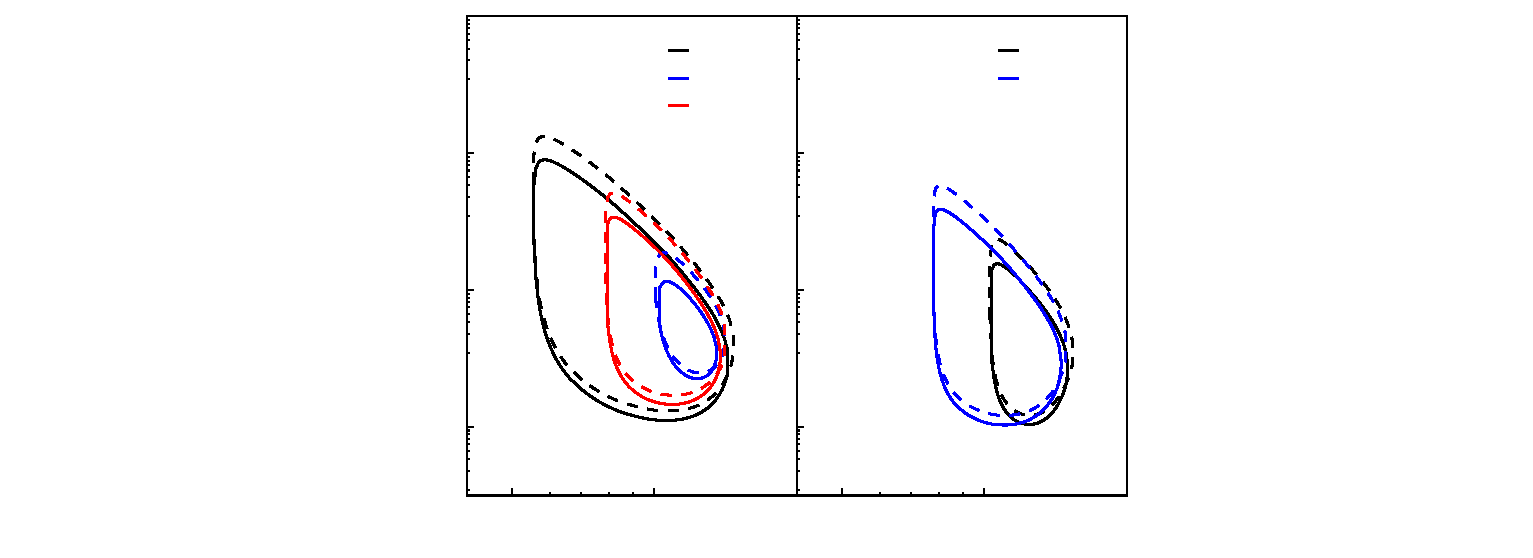
\includegraphics{pics/sensmulti_T_V2_real}}%
    \gplfronttext
  \end{picture}%
\endgroup
}}
	\caption{The 90\,\% C.L. sensitivity regions to individual channels for dominant mixings %
		$|U_{e N}|^2$ (top left), $|U_{\mu N}|^2$ (top right), and $|U_{\mu N}|^2$ (bottom) are presented for Majorana (solid lines) %
		and Dirac (dashed lines) neutrinos.
		No background analysis was performed for the channels shown here (see text).
		These channels become available only for masses above 0.5\,GeV.
	}
	\label{fig:senseV}
\end{figure}

A background study was not performed for all the other decay channels, which open up for masses above the $K^0$ mass, %
due to the fact that the final state particles need a more complex analysis.
The sensitivities to these modes are shown in~\reffig{fig:senseV}, and they can place some constraints to the mixing.
All the channels peak in their sensitivity for masses between $1.3$ and $1.8$\,GeV.
The best limits obtained for CC decays are %
$|U_{e N}|^2 < \np{2.3e-9}$ from $N \to e^\mp \rho^\pm$ and $|U_{\mu N}|^2 < \np{6.0e-8}$ from $N \to \mu^\mp \rho^\pm$; %
among the NC decays $|U_{e N}|^2 < \np{3.7e-9}$ and $|U_{\mu N}|^2 < \np{1.0e-7}$ both from $N \to \nu \phi$.
Even for these channels, there is no sensitivity to CC processes to the tau mixing, %
but interesting limits are set from $N\to \nu\eta$, $N\to \nu\omega$, and $\nu\rho^0$ to be respectively %
$|U_{\tau N}|^2 < \np{1.86e-6}$, $\np{3.24e-6}$, and~$\np{1.60e-6}$.

\subsection{Two dominant mixings}
\label{sec:bimax}

\begin{figure}
	\centering
	%{\resizebox{\linewidth}{!}{\input{pics/sens_EM.tex}}}
	{\resizebox{\linewidth}{!}{% GNUPLOT: LaTeX picture with Postscript
\begingroup
  \makeatletter
  \providecommand\color[2][]{%
    \GenericError{(gnuplot) \space\space\space\@spaces}{%
      Package color not loaded in conjunction with
      terminal option `colourtext'%
    }{See the gnuplot documentation for explanation.%
    }{Either use 'blacktext' in gnuplot or load the package
      color.sty in LaTeX.}%
    \renewcommand\color[2][]{}%
  }%
  \providecommand\includegraphics[2][]{%
    \GenericError{(gnuplot) \space\space\space\@spaces}{%
      Package graphicx or graphics not loaded%
    }{See the gnuplot documentation for explanation.%
    }{The gnuplot epslatex terminal needs graphicx.sty or graphics.sty.}%
    \renewcommand\includegraphics[2][]{}%
  }%
  \providecommand\rotatebox[2]{#2}%
  \@ifundefined{ifGPcolor}{%
    \newif\ifGPcolor
    \GPcolortrue
  }{}%
  \@ifundefined{ifGPblacktext}{%
    \newif\ifGPblacktext
    \GPblacktexttrue
  }{}%
  % define a \g@addto@macro without @ in the name:
  \let\gplgaddtomacro\g@addto@macro
  % define empty templates for all commands taking text:
  \gdef\gplbacktext{}%
  \gdef\gplfronttext{}%
  \makeatother
  \ifGPblacktext
    % no textcolor at all
    \def\colorrgb#1{}%
    \def\colorgray#1{}%
  \else
    % gray or color?
    \ifGPcolor
      \def\colorrgb#1{\color[rgb]{#1}}%
      \def\colorgray#1{\color[gray]{#1}}%
      \expandafter\def\csname LTw\endcsname{\color{white}}%
      \expandafter\def\csname LTb\endcsname{\color{black}}%
      \expandafter\def\csname LTa\endcsname{\color{black}}%
      \expandafter\def\csname LT0\endcsname{\color[rgb]{1,0,0}}%
      \expandafter\def\csname LT1\endcsname{\color[rgb]{0,1,0}}%
      \expandafter\def\csname LT2\endcsname{\color[rgb]{0,0,1}}%
      \expandafter\def\csname LT3\endcsname{\color[rgb]{1,0,1}}%
      \expandafter\def\csname LT4\endcsname{\color[rgb]{0,1,1}}%
      \expandafter\def\csname LT5\endcsname{\color[rgb]{1,1,0}}%
      \expandafter\def\csname LT6\endcsname{\color[rgb]{0,0,0}}%
      \expandafter\def\csname LT7\endcsname{\color[rgb]{1,0.3,0}}%
      \expandafter\def\csname LT8\endcsname{\color[rgb]{0.5,0.5,0.5}}%
    \else
      % gray
      \def\colorrgb#1{\color{black}}%
      \def\colorgray#1{\color[gray]{#1}}%
      \expandafter\def\csname LTw\endcsname{\color{white}}%
      \expandafter\def\csname LTb\endcsname{\color{black}}%
      \expandafter\def\csname LTa\endcsname{\color{black}}%
      \expandafter\def\csname LT0\endcsname{\color{black}}%
      \expandafter\def\csname LT1\endcsname{\color{black}}%
      \expandafter\def\csname LT2\endcsname{\color{black}}%
      \expandafter\def\csname LT3\endcsname{\color{black}}%
      \expandafter\def\csname LT4\endcsname{\color{black}}%
      \expandafter\def\csname LT5\endcsname{\color{black}}%
      \expandafter\def\csname LT6\endcsname{\color{black}}%
      \expandafter\def\csname LT7\endcsname{\color{black}}%
      \expandafter\def\csname LT8\endcsname{\color{black}}%
    \fi
  \fi
    \setlength{\unitlength}{0.0500bp}%
    \ifx\gptboxheight\undefined%
      \newlength{\gptboxheight}%
      \newlength{\gptboxwidth}%
      \newsavebox{\gptboxtext}%
    \fi%
    \setlength{\fboxrule}{0.5pt}%
    \setlength{\fboxsep}{1pt}%
\begin{picture}(14400.00,5040.00)%
    \gplgaddtomacro\gplbacktext{%
      \csname LTb\endcsname%%
      \put(444,574){\makebox(0,0)[r]{\strut{}\np{e-10}}}%
      \put(444,1467){\makebox(0,0)[r]{\strut{}\np{e-8}}}%
      \put(444,2360){\makebox(0,0)[r]{\strut{}\np{e-6}}}%
      \put(444,3253){\makebox(0,0)[r]{\strut{}\np{e-4}}}%
      \put(444,4146){\makebox(0,0)[r]{\strut{}\np{e-2}}}%
      \put(444,5039){\makebox(0,0)[r]{\strut{}\np{e0}}}%
      \put(2543,220){\makebox(0,0){\strut{}$0.5$}}%
      \put(816,220){\makebox(0,0){\strut{}$0.1$}}%
      \put(3287,220){\makebox(0,0){\strut{}$1$}}%
    }%
    \gplgaddtomacro\gplfronttext{%
      \csname LTb\endcsname%%
      \put(-436,2739){\rotatebox{-270}{\makebox(0,0){\strut{}$|U_{e N} U_{\mu N}|^2$}}}%
      \put(2303,-110){\makebox(0,0){\strut{}Mass (GeV)}}%
      \csname LTb\endcsname%%
      \put(3503,4864){\makebox(0,0)[l]{\strut{}$\nu e\mu$}}%
      \csname LTb\endcsname%%
      \put(3503,4600){\makebox(0,0)[l]{\strut{}$e\pi$}}%
      \csname LTb\endcsname%%
      \put(3503,4336){\makebox(0,0)[l]{\strut{}$\mu\pi$}}%
      \csname LTb\endcsname%%
      \put(3503,4072){\makebox(0,0)[l]{\strut{}$e K$}}%
      \csname LTb\endcsname%%
      \put(3503,3808){\makebox(0,0)[l]{\strut{}$\mu K$}}%
    }%
    \gplgaddtomacro\gplbacktext{%
      \csname LTb\endcsname%%
      \put(3900,574){\makebox(0,0)[r]{\strut{}}}%
      \put(3900,1467){\makebox(0,0)[r]{\strut{}}}%
      \put(3900,2360){\makebox(0,0)[r]{\strut{}}}%
      \put(3900,3253){\makebox(0,0)[r]{\strut{}}}%
      \put(3900,4146){\makebox(0,0)[r]{\strut{}}}%
      \put(3900,5039){\makebox(0,0)[r]{\strut{}}}%
      \put(5206,220){\makebox(0,0){\strut{}$1$}}%
    }%
    \gplgaddtomacro\gplfronttext{%
      \csname LTb\endcsname%%
      \put(5759,-110){\makebox(0,0){\strut{}Mass (GeV)}}%
      \csname LTb\endcsname%%
      \put(5665,4773){\makebox(0,0)[l]{\strut{}$e\rho$}}%
      \csname LTb\endcsname%%
      \put(5665,4509){\makebox(0,0)[l]{\strut{}$\mu\rho$}}%
      \csname LTb\endcsname%%
      \put(5665,4245){\makebox(0,0)[l]{\strut{}$e K^*$}}%
      \csname LTb\endcsname%%
      \put(5665,3981){\makebox(0,0)[l]{\strut{}$\mu K^*$}}%
    }%
    \gplgaddtomacro\gplbacktext{%
      \csname LTb\endcsname%%
      \put(7355,574){\makebox(0,0)[r]{\strut{}}}%
      \put(7355,1467){\makebox(0,0)[r]{\strut{}}}%
      \put(7355,2360){\makebox(0,0)[r]{\strut{}}}%
      \put(7355,3253){\makebox(0,0)[r]{\strut{}}}%
      \put(7355,4146){\makebox(0,0)[r]{\strut{}}}%
      \put(7355,5039){\makebox(0,0)[r]{\strut{}}}%
      \put(8537,220){\makebox(0,0){\strut{}$0.05$}}%
      \put(10039,220){\makebox(0,0){\strut{}$0.5$}}%
      \put(7487,220){\makebox(0,0){\strut{}$0.01$}}%
      \put(8989,220){\makebox(0,0){\strut{}$0.1$}}%
      \put(10491,220){\makebox(0,0){\strut{}$1$}}%
    }%
    \gplgaddtomacro\gplfronttext{%
      \csname LTb\endcsname%%
      \put(9215,-110){\makebox(0,0){\strut{}Mass (GeV)}}%
      \csname LTb\endcsname%%
      \put(8210,4773){\makebox(0,0)[l]{\strut{}$\nu e e$}}%
      \csname LTb\endcsname%%
      \put(8210,4509){\makebox(0,0)[l]{\strut{}$\nu\mu\mu$}}%
      \csname LTb\endcsname%%
      \put(8210,4245){\makebox(0,0)[l]{\strut{}$\nu\pi^0$}}%
    }%
    \gplgaddtomacro\gplbacktext{%
      \csname LTb\endcsname%%
      \put(10812,574){\makebox(0,0)[r]{\strut{}}}%
      \put(10812,1467){\makebox(0,0)[r]{\strut{}}}%
      \put(10812,2360){\makebox(0,0)[r]{\strut{}}}%
      \put(10812,3253){\makebox(0,0)[r]{\strut{}}}%
      \put(10812,4146){\makebox(0,0)[r]{\strut{}}}%
      \put(10812,5039){\makebox(0,0)[r]{\strut{}}}%
      \put(10944,220){\makebox(0,0){\strut{}$0.5$}}%
      \put(14399,220){\makebox(0,0){\strut{}$2$}}%
      \put(12672,220){\makebox(0,0){\strut{}$1$}}%
    }%
    \gplgaddtomacro\gplfronttext{%
      \csname LTb\endcsname%%
      \put(12671,-110){\makebox(0,0){\strut{}Mass (GeV)}}%
      \csname LTb\endcsname%%
      \put(14003,4773){\makebox(0,0)[l]{\strut{}$\nu\eta$}}%
      \csname LTb\endcsname%%
      \put(14003,4509){\makebox(0,0)[l]{\strut{}$\nu\eta'$}}%
      \csname LTb\endcsname%%
      \put(14003,4245){\makebox(0,0)[l]{\strut{}$\nu\rho^0$}}%
      \csname LTb\endcsname%%
      \put(14003,3981){\makebox(0,0)[l]{\strut{}$\nu\omega$}}%
      \csname LTb\endcsname%%
      \put(14003,3717){\makebox(0,0)[l]{\strut{}$\nu\phi$}}%
    }%
    \gplbacktext
    \put(0,0){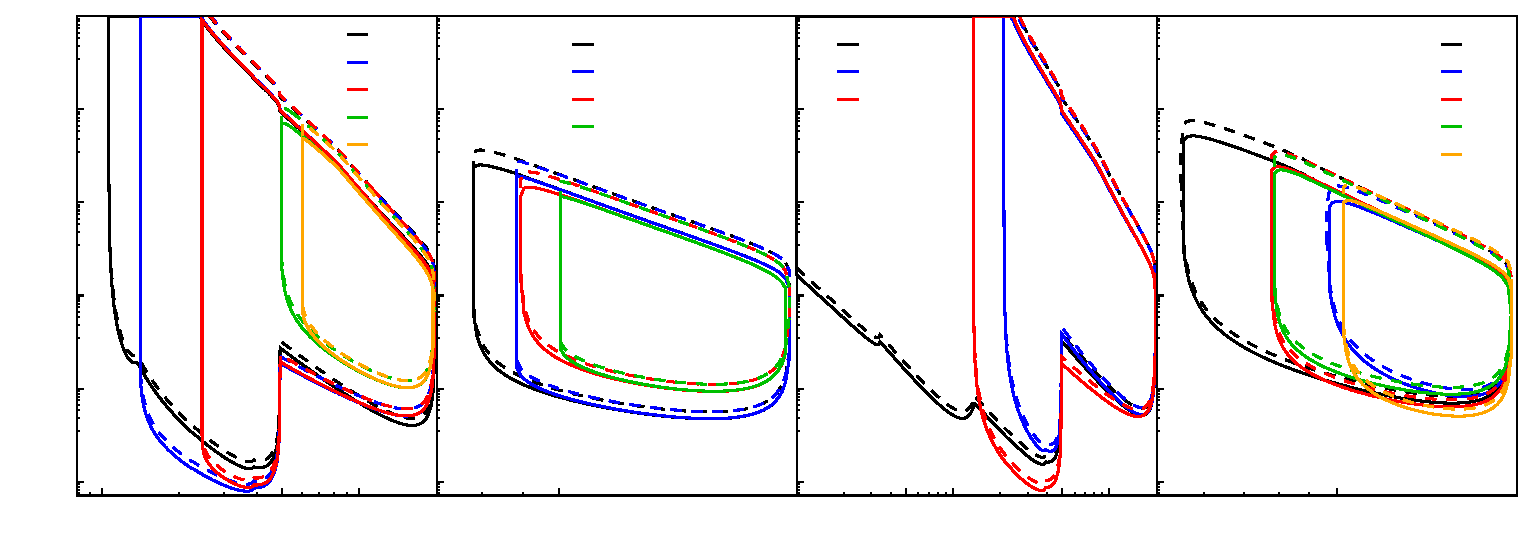
\includegraphics{pics/sensmulti_EM2_real}}%
    \gplfronttext
  \end{picture}%
\endgroup
}}
	\vspace{0.05em}

	%{\resizebox{\linewidth}{!}{\input{pics/sens_MT.tex}}}
	{\resizebox{\linewidth}{!}{% GNUPLOT: LaTeX picture with Postscript
\begingroup
  \makeatletter
  \providecommand\color[2][]{%
    \GenericError{(gnuplot) \space\space\space\@spaces}{%
      Package color not loaded in conjunction with
      terminal option `colourtext'%
    }{See the gnuplot documentation for explanation.%
    }{Either use 'blacktext' in gnuplot or load the package
      color.sty in LaTeX.}%
    \renewcommand\color[2][]{}%
  }%
  \providecommand\includegraphics[2][]{%
    \GenericError{(gnuplot) \space\space\space\@spaces}{%
      Package graphicx or graphics not loaded%
    }{See the gnuplot documentation for explanation.%
    }{The gnuplot epslatex terminal needs graphicx.sty or graphics.sty.}%
    \renewcommand\includegraphics[2][]{}%
  }%
  \providecommand\rotatebox[2]{#2}%
  \@ifundefined{ifGPcolor}{%
    \newif\ifGPcolor
    \GPcolortrue
  }{}%
  \@ifundefined{ifGPblacktext}{%
    \newif\ifGPblacktext
    \GPblacktexttrue
  }{}%
  % define a \g@addto@macro without @ in the name:
  \let\gplgaddtomacro\g@addto@macro
  % define empty templates for all commands taking text:
  \gdef\gplbacktext{}%
  \gdef\gplfronttext{}%
  \makeatother
  \ifGPblacktext
    % no textcolor at all
    \def\colorrgb#1{}%
    \def\colorgray#1{}%
  \else
    % gray or color?
    \ifGPcolor
      \def\colorrgb#1{\color[rgb]{#1}}%
      \def\colorgray#1{\color[gray]{#1}}%
      \expandafter\def\csname LTw\endcsname{\color{white}}%
      \expandafter\def\csname LTb\endcsname{\color{black}}%
      \expandafter\def\csname LTa\endcsname{\color{black}}%
      \expandafter\def\csname LT0\endcsname{\color[rgb]{1,0,0}}%
      \expandafter\def\csname LT1\endcsname{\color[rgb]{0,1,0}}%
      \expandafter\def\csname LT2\endcsname{\color[rgb]{0,0,1}}%
      \expandafter\def\csname LT3\endcsname{\color[rgb]{1,0,1}}%
      \expandafter\def\csname LT4\endcsname{\color[rgb]{0,1,1}}%
      \expandafter\def\csname LT5\endcsname{\color[rgb]{1,1,0}}%
      \expandafter\def\csname LT6\endcsname{\color[rgb]{0,0,0}}%
      \expandafter\def\csname LT7\endcsname{\color[rgb]{1,0.3,0}}%
      \expandafter\def\csname LT8\endcsname{\color[rgb]{0.5,0.5,0.5}}%
    \else
      % gray
      \def\colorrgb#1{\color{black}}%
      \def\colorgray#1{\color[gray]{#1}}%
      \expandafter\def\csname LTw\endcsname{\color{white}}%
      \expandafter\def\csname LTb\endcsname{\color{black}}%
      \expandafter\def\csname LTa\endcsname{\color{black}}%
      \expandafter\def\csname LT0\endcsname{\color{black}}%
      \expandafter\def\csname LT1\endcsname{\color{black}}%
      \expandafter\def\csname LT2\endcsname{\color{black}}%
      \expandafter\def\csname LT3\endcsname{\color{black}}%
      \expandafter\def\csname LT4\endcsname{\color{black}}%
      \expandafter\def\csname LT5\endcsname{\color{black}}%
      \expandafter\def\csname LT6\endcsname{\color{black}}%
      \expandafter\def\csname LT7\endcsname{\color{black}}%
      \expandafter\def\csname LT8\endcsname{\color{black}}%
    \fi
  \fi
    \setlength{\unitlength}{0.0500bp}%
    \ifx\gptboxheight\undefined%
      \newlength{\gptboxheight}%
      \newlength{\gptboxwidth}%
      \newsavebox{\gptboxtext}%
    \fi%
    \setlength{\fboxrule}{0.5pt}%
    \setlength{\fboxsep}{1pt}%
\begin{picture}(14400.00,5040.00)%
    \gplgaddtomacro\gplbacktext{%
      \csname LTb\endcsname%%
      \put(444,574){\makebox(0,0)[r]{\strut{}\np{e-10}}}%
      \put(444,1467){\makebox(0,0)[r]{\strut{}\np{e-8}}}%
      \put(444,2360){\makebox(0,0)[r]{\strut{}\np{e-6}}}%
      \put(444,3253){\makebox(0,0)[r]{\strut{}\np{e-4}}}%
      \put(444,4146){\makebox(0,0)[r]{\strut{}\np{e-2}}}%
      \put(444,5039){\makebox(0,0)[r]{\strut{}\np{1}}}%
      \put(2543,220){\makebox(0,0){\strut{}$0.5$}}%
      \put(816,220){\makebox(0,0){\strut{}$0.1$}}%
      \put(3287,220){\makebox(0,0){\strut{}$1$}}%
    }%
    \gplgaddtomacro\gplfronttext{%
      \csname LTb\endcsname%%
      \put(-436,2739){\rotatebox{-270}{\makebox(0,0){\strut{}$|U_{\mu N} U_{\tau N}|^2$}}}%
      \put(2303,-110){\makebox(0,0){\strut{}Mass $m_N$ (GeV)}}%
      \csname LTb\endcsname%%
      \put(3371,4844){\makebox(0,0)[l]{\strut{}$\nu e\mu$}}%
      \csname LTb\endcsname%%
      \put(3371,4580){\makebox(0,0)[l]{\strut{}$\mu\pi$}}%
      \csname LTb\endcsname%%
      \put(3371,4316){\makebox(0,0)[l]{\strut{}$\mu K$}}%
    }%
    \gplgaddtomacro\gplbacktext{%
      \csname LTb\endcsname%%
      \put(3900,574){\makebox(0,0)[r]{\strut{}}}%
      \put(3900,1467){\makebox(0,0)[r]{\strut{}}}%
      \put(3900,2360){\makebox(0,0)[r]{\strut{}}}%
      \put(3900,3253){\makebox(0,0)[r]{\strut{}}}%
      \put(3900,4146){\makebox(0,0)[r]{\strut{}}}%
      \put(3900,5039){\makebox(0,0)[r]{\strut{}}}%
      \put(5206,220){\makebox(0,0){\strut{}$1$}}%
    }%
    \gplgaddtomacro\gplfronttext{%
      \csname LTb\endcsname%%
      \put(5759,-110){\makebox(0,0){\strut{}Mass $m_N$ (GeV)}}%
      \csname LTb\endcsname%%
      \put(6827,4844){\makebox(0,0)[l]{\strut{}$e\rho$}}%
      \csname LTb\endcsname%%
      \put(6827,4580){\makebox(0,0)[l]{\strut{}$e K^*$}}%
    }%
    \gplgaddtomacro\gplbacktext{%
      \csname LTb\endcsname%%
      \put(7355,574){\makebox(0,0)[r]{\strut{}}}%
      \put(7355,1467){\makebox(0,0)[r]{\strut{}}}%
      \put(7355,2360){\makebox(0,0)[r]{\strut{}}}%
      \put(7355,3253){\makebox(0,0)[r]{\strut{}}}%
      \put(7355,4146){\makebox(0,0)[r]{\strut{}}}%
      \put(7355,5039){\makebox(0,0)[r]{\strut{}}}%
      \put(7487,220){\makebox(0,0){\strut{}$0.01$}}%
      \put(8989,220){\makebox(0,0){\strut{}$0.1$}}%
      \put(10491,220){\makebox(0,0){\strut{}$1$}}%
    }%
    \gplgaddtomacro\gplfronttext{%
      \csname LTb\endcsname%%
      \put(9215,-110){\makebox(0,0){\strut{}Mass $m_N$ (GeV)}}%
      \csname LTb\endcsname%%
      \put(8078,4844){\makebox(0,0)[l]{\strut{}$\nu e e$}}%
      \csname LTb\endcsname%%
      \put(8078,4580){\makebox(0,0)[l]{\strut{}$\nu\mu\mu$}}%
      \csname LTb\endcsname%%
      \put(8078,4316){\makebox(0,0)[l]{\strut{}$\nu\pi^0$}}%
    }%
    \gplgaddtomacro\gplbacktext{%
      \csname LTb\endcsname%%
      \put(10812,574){\makebox(0,0)[r]{\strut{}}}%
      \put(10812,1467){\makebox(0,0)[r]{\strut{}}}%
      \put(10812,2360){\makebox(0,0)[r]{\strut{}}}%
      \put(10812,3253){\makebox(0,0)[r]{\strut{}}}%
      \put(10812,4146){\makebox(0,0)[r]{\strut{}}}%
      \put(10812,5039){\makebox(0,0)[r]{\strut{}}}%
      \put(14399,220){\makebox(0,0){\strut{}$2$}}%
      \put(12672,220){\makebox(0,0){\strut{}$1$}}%
    }%
    \gplgaddtomacro\gplfronttext{%
      \csname LTb\endcsname%%
      \put(12671,-110){\makebox(0,0){\strut{}Mass $m_N$ (GeV)}}%
      \csname LTb\endcsname%%
      \put(13871,4844){\makebox(0,0)[l]{\strut{}$\nu\eta$}}%
      \csname LTb\endcsname%%
      \put(13871,4580){\makebox(0,0)[l]{\strut{}$\nu\eta'$}}%
      \csname LTb\endcsname%%
      \put(13871,4316){\makebox(0,0)[l]{\strut{}$\nu\rho^0$}}%
      \csname LTb\endcsname%%
      \put(13871,4052){\makebox(0,0)[l]{\strut{}$\nu\omega$}}%
      \csname LTb\endcsname%%
      \put(13871,3788){\makebox(0,0)[l]{\strut{}$\nu\phi$}}%
    }%
    \gplbacktext
    \put(0,0){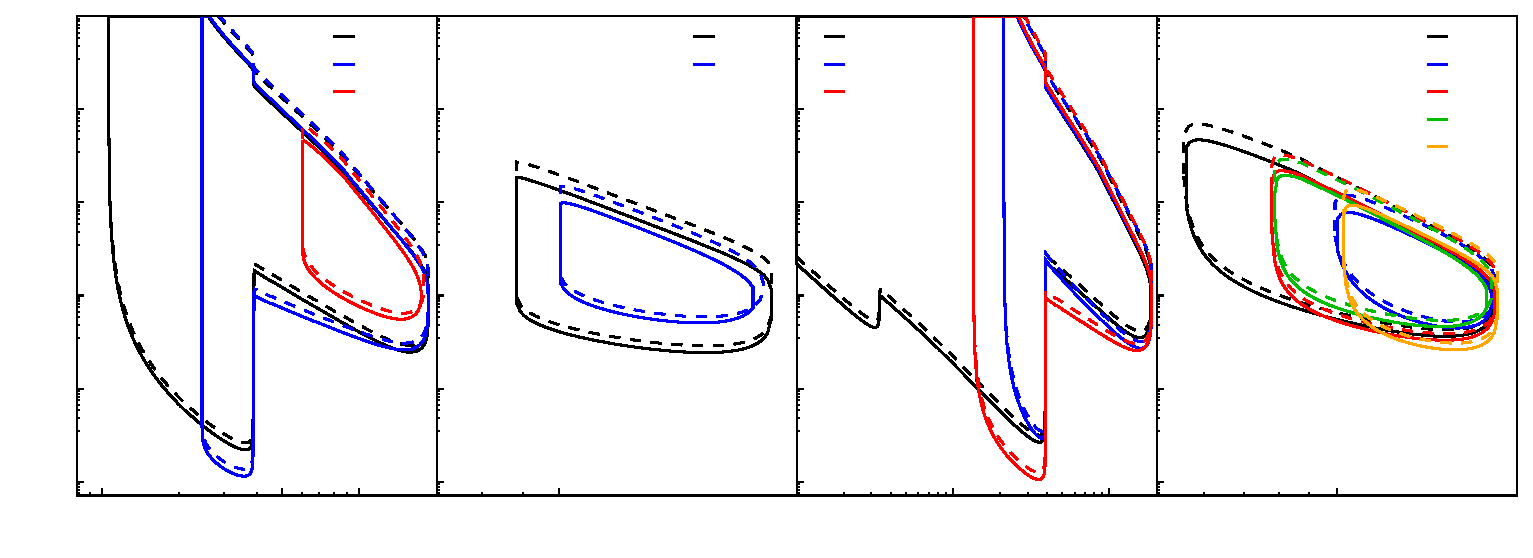
\includegraphics{pics/sensmulti_MT2_real}}%
    \gplfronttext
  \end{picture}%
\endgroup
}}
	\vspace{0.05em}

	%{\resizebox{\linewidth}{!}{\input{pics/sens_TE.tex}}}
	{\resizebox{\linewidth}{!}{% GNUPLOT: LaTeX picture with Postscript
\begingroup
  \makeatletter
  \providecommand\color[2][]{%
    \GenericError{(gnuplot) \space\space\space\@spaces}{%
      Package color not loaded in conjunction with
      terminal option `colourtext'%
    }{See the gnuplot documentation for explanation.%
    }{Either use 'blacktext' in gnuplot or load the package
      color.sty in LaTeX.}%
    \renewcommand\color[2][]{}%
  }%
  \providecommand\includegraphics[2][]{%
    \GenericError{(gnuplot) \space\space\space\@spaces}{%
      Package graphicx or graphics not loaded%
    }{See the gnuplot documentation for explanation.%
    }{The gnuplot epslatex terminal needs graphicx.sty or graphics.sty.}%
    \renewcommand\includegraphics[2][]{}%
  }%
  \providecommand\rotatebox[2]{#2}%
  \@ifundefined{ifGPcolor}{%
    \newif\ifGPcolor
    \GPcolortrue
  }{}%
  \@ifundefined{ifGPblacktext}{%
    \newif\ifGPblacktext
    \GPblacktexttrue
  }{}%
  % define a \g@addto@macro without @ in the name:
  \let\gplgaddtomacro\g@addto@macro
  % define empty templates for all commands taking text:
  \gdef\gplbacktext{}%
  \gdef\gplfronttext{}%
  \makeatother
  \ifGPblacktext
    % no textcolor at all
    \def\colorrgb#1{}%
    \def\colorgray#1{}%
  \else
    % gray or color?
    \ifGPcolor
      \def\colorrgb#1{\color[rgb]{#1}}%
      \def\colorgray#1{\color[gray]{#1}}%
      \expandafter\def\csname LTw\endcsname{\color{white}}%
      \expandafter\def\csname LTb\endcsname{\color{black}}%
      \expandafter\def\csname LTa\endcsname{\color{black}}%
      \expandafter\def\csname LT0\endcsname{\color[rgb]{1,0,0}}%
      \expandafter\def\csname LT1\endcsname{\color[rgb]{0,1,0}}%
      \expandafter\def\csname LT2\endcsname{\color[rgb]{0,0,1}}%
      \expandafter\def\csname LT3\endcsname{\color[rgb]{1,0,1}}%
      \expandafter\def\csname LT4\endcsname{\color[rgb]{0,1,1}}%
      \expandafter\def\csname LT5\endcsname{\color[rgb]{1,1,0}}%
      \expandafter\def\csname LT6\endcsname{\color[rgb]{0,0,0}}%
      \expandafter\def\csname LT7\endcsname{\color[rgb]{1,0.3,0}}%
      \expandafter\def\csname LT8\endcsname{\color[rgb]{0.5,0.5,0.5}}%
    \else
      % gray
      \def\colorrgb#1{\color{black}}%
      \def\colorgray#1{\color[gray]{#1}}%
      \expandafter\def\csname LTw\endcsname{\color{white}}%
      \expandafter\def\csname LTb\endcsname{\color{black}}%
      \expandafter\def\csname LTa\endcsname{\color{black}}%
      \expandafter\def\csname LT0\endcsname{\color{black}}%
      \expandafter\def\csname LT1\endcsname{\color{black}}%
      \expandafter\def\csname LT2\endcsname{\color{black}}%
      \expandafter\def\csname LT3\endcsname{\color{black}}%
      \expandafter\def\csname LT4\endcsname{\color{black}}%
      \expandafter\def\csname LT5\endcsname{\color{black}}%
      \expandafter\def\csname LT6\endcsname{\color{black}}%
      \expandafter\def\csname LT7\endcsname{\color{black}}%
      \expandafter\def\csname LT8\endcsname{\color{black}}%
    \fi
  \fi
    \setlength{\unitlength}{0.0500bp}%
    \ifx\gptboxheight\undefined%
      \newlength{\gptboxheight}%
      \newlength{\gptboxwidth}%
      \newsavebox{\gptboxtext}%
    \fi%
    \setlength{\fboxrule}{0.5pt}%
    \setlength{\fboxsep}{1pt}%
\begin{picture}(14400.00,5040.00)%
    \gplgaddtomacro\gplbacktext{%
      \csname LTb\endcsname%%
      \put(444,574){\makebox(0,0)[r]{\strut{}\np{e-10}}}%
      \put(444,1467){\makebox(0,0)[r]{\strut{}\np{e-8}}}%
      \put(444,2360){\makebox(0,0)[r]{\strut{}\np{e-6}}}%
      \put(444,3253){\makebox(0,0)[r]{\strut{}\np{e-4}}}%
      \put(444,4146){\makebox(0,0)[r]{\strut{}\np{e-2}}}%
      \put(444,5039){\makebox(0,0)[r]{\strut{}\np{e0}}}%
      \put(2543,220){\makebox(0,0){\strut{}$0.5$}}%
      \put(816,220){\makebox(0,0){\strut{}$0.1$}}%
      \put(3287,220){\makebox(0,0){\strut{}$1$}}%
    }%
    \gplgaddtomacro\gplfronttext{%
      \csname LTb\endcsname%%
      \put(-436,2739){\rotatebox{-270}{\makebox(0,0){\strut{}$|U_{e N} U_{\tau N}|^2$}}}%
      \put(2303,-110){\makebox(0,0){\strut{}Mass (GeV)}}%
      \csname LTb\endcsname%%
      \put(3371,4844){\makebox(0,0)[l]{\strut{}$\nu e\mu$}}%
      \csname LTb\endcsname%%
      \put(3371,4580){\makebox(0,0)[l]{\strut{}$e\pi$}}%
      \csname LTb\endcsname%%
      \put(3371,4316){\makebox(0,0)[l]{\strut{}$e K$}}%
    }%
    \gplgaddtomacro\gplbacktext{%
      \csname LTb\endcsname%%
      \put(3900,574){\makebox(0,0)[r]{\strut{}}}%
      \put(3900,1467){\makebox(0,0)[r]{\strut{}}}%
      \put(3900,2360){\makebox(0,0)[r]{\strut{}}}%
      \put(3900,3253){\makebox(0,0)[r]{\strut{}}}%
      \put(3900,4146){\makebox(0,0)[r]{\strut{}}}%
      \put(3900,5039){\makebox(0,0)[r]{\strut{}}}%
      \put(5206,220){\makebox(0,0){\strut{}$1$}}%
    }%
    \gplgaddtomacro\gplfronttext{%
      \csname LTb\endcsname%%
      \put(5759,-110){\makebox(0,0){\strut{}Mass (GeV)}}%
      \csname LTb\endcsname%%
      \put(6827,4844){\makebox(0,0)[l]{\strut{}$e\rho$}}%
      \csname LTb\endcsname%%
      \put(6827,4580){\makebox(0,0)[l]{\strut{}$e K^*$}}%
    }%
    \gplgaddtomacro\gplbacktext{%
      \csname LTb\endcsname%%
      \put(7355,574){\makebox(0,0)[r]{\strut{}}}%
      \put(7355,1467){\makebox(0,0)[r]{\strut{}}}%
      \put(7355,2360){\makebox(0,0)[r]{\strut{}}}%
      \put(7355,3253){\makebox(0,0)[r]{\strut{}}}%
      \put(7355,4146){\makebox(0,0)[r]{\strut{}}}%
      \put(7355,5039){\makebox(0,0)[r]{\strut{}}}%
      \put(7487,220){\makebox(0,0){\strut{}$0.01$}}%
      \put(8989,220){\makebox(0,0){\strut{}$0.1$}}%
      \put(10491,220){\makebox(0,0){\strut{}$1$}}%
    }%
    \gplgaddtomacro\gplfronttext{%
      \csname LTb\endcsname%%
      \put(9215,-110){\makebox(0,0){\strut{}Mass (GeV)}}%
      \csname LTb\endcsname%%
      \put(8078,4844){\makebox(0,0)[l]{\strut{}$\nu e e$}}%
      \csname LTb\endcsname%%
      \put(8078,4580){\makebox(0,0)[l]{\strut{}$\nu\mu\mu$}}%
      \csname LTb\endcsname%%
      \put(8078,4316){\makebox(0,0)[l]{\strut{}$\nu\pi^0$}}%
    }%
    \gplgaddtomacro\gplbacktext{%
      \csname LTb\endcsname%%
      \put(10812,574){\makebox(0,0)[r]{\strut{}}}%
      \put(10812,1467){\makebox(0,0)[r]{\strut{}}}%
      \put(10812,2360){\makebox(0,0)[r]{\strut{}}}%
      \put(10812,3253){\makebox(0,0)[r]{\strut{}}}%
      \put(10812,4146){\makebox(0,0)[r]{\strut{}}}%
      \put(10812,5039){\makebox(0,0)[r]{\strut{}}}%
      \put(14399,220){\makebox(0,0){\strut{}$2$}}%
      \put(12672,220){\makebox(0,0){\strut{}$1$}}%
    }%
    \gplgaddtomacro\gplfronttext{%
      \csname LTb\endcsname%%
      \put(12671,-110){\makebox(0,0){\strut{}Mass (GeV)}}%
      \csname LTb\endcsname%%
      \put(13871,4844){\makebox(0,0)[l]{\strut{}$\nu\eta$}}%
      \csname LTb\endcsname%%
      \put(13871,4580){\makebox(0,0)[l]{\strut{}$\nu\eta'$}}%
      \csname LTb\endcsname%%
      \put(13871,4316){\makebox(0,0)[l]{\strut{}$\nu\rho^0$}}%
      \csname LTb\endcsname%%
      \put(13871,4052){\makebox(0,0)[l]{\strut{}$\nu\omega$}}%
      \csname LTb\endcsname%%
      \put(13871,3788){\makebox(0,0)[l]{\strut{}$\nu\phi$}}%
    }%
    \gplbacktext
    \put(0,0){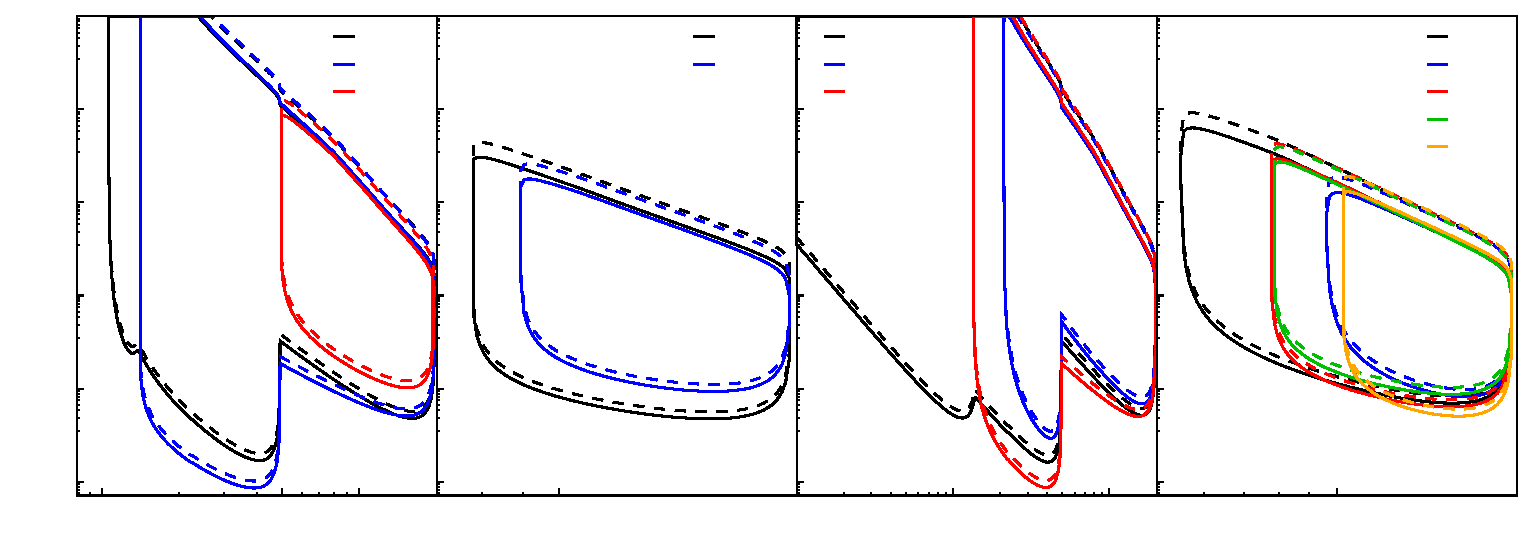
\includegraphics{pics/sensmulti_TE2_real}}%
    \gplfronttext
  \end{picture}%
\endgroup
}}
	\caption{The 90\,\% C.L. sensitivity regions to individual channels for two dominant mixings %
		$|U_{e N}^* U_{\mu N}|$ (top), $|U_{\mu N}^* U_{\tau N}|$ (middle), and $|U_{e N}^* U_{\tau N}|$ (bottom) are presented.
		All the modes considered in this work are shown here, but no background analysis is reported.
		As before, the solid lines correspond to the analysis with Majorana neutrinos, the dashed lines with Dirac neutrino.}
	\label{fig:senseMix}
\end{figure}

In this section we present the bounds in a scenario in which two mixing elements are comparable and dominant over the third one.
This case complements the previous analysis in \refsec{sec:dominant} as, by searching for HNL decays, %
the experiment can constrain certain combinations of the mixing elements.
This can happen when the neutrino is produced via one mixing and decays via another one, %
or when both mixing elements play a role in production and decay.
For instance, the decay $K^+ \to \mu^+ N$ yields heavy neutrinos with a flux proportional to %
$|U_{\mu N}|^2$, but they can afterwards decay into the channel $\nu e^+ e^-$ also via the electronic or the tau mixing.
It is important to highlight that, in the case in which one mixing is responsible %
for the production and a different mixing for the decay, %
then number of events is proportional to the product of the mixings %
$|U_{\alpha N}||U_{\beta N}|$ if the studied channel is CC--mediated.
However, if the decay channel is also sensitive to a NC exchange, the number of events is instead proportional to %
$|U_{\alpha N}|\sqrt{|U_{\alpha N}|^2 + |U_{\beta N}|^2}$.
In the remainder of this section, we will use the combination of two mixings represented by $|U_{\alpha N}^* U_{\beta N}|$ %
\enlargethispage{\baselineskip}
for comparing bounds and sensitivity plots.

%However, if two mixings are non-zero, nothing prevents the production and the decay to be mediated by both of them. 
The combinations of mixing terms is relevant to charged Lepton Flavour Violating (cLFV) %
decays or flavour changing neutral current processes %
which can be enhanced in presence of nearly-sterile neutrinos.
For example, the well-known decay $\mu^+ \to e^+ \gamma$ has a branching ratio which is sensitive to extra neutrino states.
This reads
\begin{equation}
	\label{eq:meg}
	\text{Br}(\mu^+ \to e^+ \gamma) = \frac{3 \alpha}{32 \pi} \abs{\sum_i \hat{U}_{\mu i}^*\, \hat{U}_{e i}\,G\qty(\frac{m_i^2}{M_W^2})} \ ,
\end{equation}
where $G(x)$ is the loop function of the process~\cite{Ilakovac:1994kj}.
The current upper limit is set by the MEG experiment to be %
$\text{Br}(\mu^+ \to e^+\gamma) < \np{4.2e-13}$~\cite{TheMEG:2016wtm}.
Despite being one of the best constrained cLFV process, the bounds on $|U_{e N}^* U_{\mu N}|$ are not as good as the ones imposed %
by other processes, like $\mu \to e e e$ or $\mu - e$ conversion on nuclei~\cite{Alonso:2012ji}.
For instance, the constraint from conversion on Au is $|U_{e N}^* U_{\mu N}| < \np{1.6e-5}$ %
for HNL masses larger than 0.1\,GeV~\cite{Deshpande:2011uv}.
The branching ratio of other cLFV channels, like $\tau \to e \gamma$ or $\tau \to \mu \gamma$ are not as well constrained %
and so the bounds achievable on the combination of heavy neutrino mixings are expected to be less %
stringent~\cite{Buras:2010cp, Abada:2016vzu}.
Stronger bounds come from study of three-body decays of charm and bottom mesons to charged leptons with different flavour %
and tau decays to pseudo-scalar mesons and a charged lepton: from the search for %
the decay $K \to e \mu \pi$ the bound $|U_{e N}^* U_{\mu N}| < \np{e-9}$ is reached for masses %
$0.15\,\text{GeV}\lesssim m_N \lesssim 0.50\,\text{GeV}$;
%\enlargethispage{\baselineskip}
the decays $\tau \to e \pi \pi$ and $\tau \to \mu \pi\pi$ set the limits %
$|U_{e N}^* U_{\tau N}|, |U_{\mu N}^* U_{\tau N}| < \np{5e-6}$ for the respective mass ranges %
$0.14\,\text{GeV}\lesssim m_N \lesssim 1.7\,\text{GeV}$ and %
$0.24\,\text{GeV}\lesssim m_N \lesssim 1.7\,\text{GeV}$~\cite{Helo:2010cw}.



Instead of dealing with a three-dimensional parameter scan, we simplify the study %
by assigning the same value to the two mixing parameters under consideration, for which the number %
of HNL decays is maximal.
The number of events is then reported as a function of the neutrino mass and the combination $|U_{\alpha N}^* U_{\beta N}|$.
The results for all channels considered in this work are shown in~\reffig{fig:senseMix}.
The best constraints come again from two-body semi-leptonic decays for all mixing combinations, %
the lowest upper limits being $|U_{e N}^* U_{\mu N}| < \np{6e-11}$ at $m_N \simeq 0.36$\,GeV, %
$|U_{\mu N}^* U_{\tau N}| < \np{1.3e-10}$ at $m_N \simeq 0.35$\,GeV, %
and $|U_{\tau N}^* U_{e N}| < \np{7e-11}$ at $m_N \simeq 0.39$\,GeV.
Amongst the three-body leptonic decay channels, $N\to\nu e e$ has the best sensitivity for masses $m_N < m_{K^0}$, %
but actually the mode $N\to \nu e^\mp \mu^\pm$ can be more constraining at higher masses.
Regarding the channels available only above the kaon mass threshold, decays to pseudo-scalar mesons are the most sensitive %
between C processes, whereas the decay $N \to \nu \phi$ gives the best constraint of the NC--mediated channels.
\section{Mass model constraints from DUNE ND}
\label{sec:combined}

%Finally, we make a comparison of this analysis with previous and recent results of beam dump experiment.
%and explain the how the experiment %
%can explore the parameter spaces of different neutrino mass models in the next section, \ref{sec:combined}.

From the results presented in the previous section, we find that the DUNE ND will be sensitive to very low couplings %
for experimentally accessible mass values.
These points of the parameter space corresponds to regions viable in some realisations of low scale neutrino mass models.
In view of the discussion regarding seesaw models in \refsec{sec:model}, we perform a mass matrix random scan to %
define such regions of the parameter space.
Following the previously introduced notation, we focus on three minimal ISS scenarios which predict a HNL with a mass accessible %
by the experiment and that satisfy the experimental evidence of neutrino oscillation~\cite{Abada:2014vea}.
In the first two cases, the heavy neutrino under study belongs to the lightest pseudo-Dirac pair %
of an ISS\,(2,2) and an ISS\,(2,3) realisation; the third scenario is an ISS\,(2,3) case %
in which the fourth Weyl state becomes a Majorana neutrino in the \mbox{MeV--GeV} region thanks to a high LNV parameter.
The details of this analysis are reported in this section, together with the overall sensitivities of DUNE ND to %
heavy neutrino discovery and low scale mass models. 
A comparison with future experiments is also included.

\subsection{Mass model scan}

%The DUNE experiment will be very sensitive to regions of the parameter space of interest with respect to low scale seesaw models.
We have randomly generated neutrino mass matrices and numerically diagonalised them.
The structure of the mass matrix is a generalised version of an ISS:
\begin{equation}
	\mathcal{M} = 
	\begin{pmatrix}
		0	& m_D^T	& 0	\\
		m_D	& \mu_R	& M^T_R	\\
		0	& M_R	& \mu_S
	\end{pmatrix}\ ,
\end{equation}
with two LNV submatrices, $\mu_R$ and $\mu_S$.
The number of physical parameters of a ISS\,$(a,b)$ mass matrix is $n_p = 7a + b +2 a\,b$~\cite{Abada:2014vea}. %
We choose a basis in which $m_D$ has complex entries but three of which are real, $M_R$ is diagonal and real, and $\mu_S$ has a real diagonal %
without loss of generality.
If the matrix entries respect the hierarchy \mbox{$\mu_{R,S} \ll m_D \ll M_R$}, the mass spectrum in %
the LNC limit is principally given by the diagonal values of $M_R$.
We then perturb the matrix to achieve the three minimal ISS scenarios introduced above; %
the randomly generated mass matrix $\mathcal{M}$ %
is then diagonalised using the Jacobi Singular Value Decomposition (SVD) as implemented in the Eigen library~\cite{Eigen:2010}.
The Takagi decomposition, %
\begin{equation*}
	\hat{U}^T \mathcal{M}\, \hat{U} = \text{diag}(m_1, m_2, m_3, ...)\ ,
\end{equation*}
is retrieved starting from the SVD decomposition $\mathcal{M} = V \Sigma U^\dagger$, %
from which the singular values $\Sigma$ are the non-negative square roots of the eigenvalues of $\mathcal{M}^\dagger \mathcal{M}$ %
and the unitary matrix is $\hat{U} = U \rho^\dagger$, where $\rho = (U^T V)^\frac{1}{2}$ is a unitary phase matrix.

Only matrices satisfying the current constraints on heavy neutral fermions are taken in account.
The first requirement is that the eigenvalues must give the correct mass squared splittings %
compatible within 3$\sigma$ with the measured values~\cite{Esteban:2018azc}.
The condition of matching also the measured mixing angles is relaxed because %
the entries of the PMNS matrix, $\mathcal{U}$, are the result of the random structure of $m_D$ and $\mu_S$.
Constraints on the unitarity of the mixing matrix are applied instead.
The deviation from unitarity are quantified by the following Hermitian matrix:
\begin{equation}
	\varepsilon_{\alpha \beta} \equiv |\delta_{\alpha \beta} - (\mathcal{U}\,\mathcal{U}^\dagger)_{\alpha \beta}| = %
	\abs{\sum_{i=4}^n \hat{U}_{\alpha i} \hat{U}_{\beta i}^*}\ .
\end{equation}
The non-unitarity of the PMNS matrix has been assessed in various experiments, and the constraints depend upon the mass scale of averaged out neutrinos.
For neutrino masses below the GeV scale, but heavy enough to decouple from flavour oscillations, %
non-unitarity effects are tested in neutrino oscillation experiment as an overall normalisation.
If the neutrino mass is above the GeV scale, electroweak precision experiments provide strong constraints on non-unitarity.
The constraints are summarised below (from~\refref{Antusch:2008tz, Fernandez-Martinez:2016lgt, Blennow:2016jkn})
\begin{align*}
	&\varepsilon_{\alpha \beta} <
	\begin{pmatrix}
		\np{2.4e-2}	& \np{1.3e-2}	& \np{3.5e-2}	\\
		\cdot		& \np{2.2e-2}	& \np{6.0e-3}	\\
		\cdot		& \cdot		& \np{1.0e-1}
	\end{pmatrix}\quad 
	\text{if 10\,eV} \lesssim m_N \lesssim \text{1\,GeV}\ ,\\
	&\varepsilon_{\alpha \beta} <
	\begin{pmatrix}
		\np{1.3e-3}	& \np{1.2e-5}	& \np{1.4e-3}	\\
		\cdot		& \np{2.2e-4}	& \np{6.0e-4}	\\
		\cdot		& \cdot		& \np{2.8e-3}
	\end{pmatrix}\quad
	\text{if}\ m_N \gtrsim \text{1\,GeV}\ .
\end{align*}

The $\mu_R$ and $\mu_S$ entries of the ISS matrices naturally lead to lepton flavour and lepton number violating processes.
The most constrained process is the decay rate of \mbox{$\mu^+ \to e^+\gamma$}, the branching ratio of which is given in \refeq{eq:meg}.
The current upper limit on the branching ratio is \np{4.2e-13}, but a future upgrade of the experiment %
foresees to reach a limit lower than \np{5e-14}.

Heavy neutrinos in a ISS model also contribute to the neutrinoless double beta decay.
The effective neutrino mass $m_{\beta\beta}$ receives further corrections with respect %
to the standard expression as
\begin{equation}
	m_{\beta\beta} \simeq \abs{\sum_i \hat{U}_{e i}^2 \frac{p^2\,m_i}{p^2 - m_i^2}}
\end{equation}
where $p^2 \simeq -\np{0.015}$\,GeV\tapi{2} is the typical virtual momentum of the exchanged neutrino.
The~contribution from masses above the 0.1\,GeV scale drops as $\flatfrac{1}{m^2_i}$ while it is constant for masses below~\cite{Blennow:2010th}.
It is interesting to note that the contributions given by pseudo-Dirac pairs are subject to partial cancellation, regulated by the LNV parameters.
In the LNC limit, the cancellation is maximum and the paired states do not take part in the $0\nu\beta\beta$ process.
The latest result from the KamLAND-Zen experiment~\cite{KamLAND-Zen:2016pfg} is interpreted as~\mbox{$m_{\beta\beta} < 61$\,meV}.
%The latest result from the GERDA experiment~\cite{Agostini:2017iyd} is interpreted as $m_{\beta\beta} < 150$\,meV.

We find, for the first two ISS scenarios, that the allowed ranges span in the space %
\mbox{$m_D \sim 10^{[3,6]}$\,eV}, \mbox{$M_R \sim 10^{[6,15]}$\,eV}, $\mu_S$ and $\mu_R \sim 10^{[-4,1]}$\,eV.
We check that each matrix generated respects the \emph{naturalness condition} in the 't Hooft sense~\cite{tHooft:1980xss} %
and that the mass spectrum presents a mass state accessible by the DUNE experiment.
For the third ISS case, large entries of the sub-matrix $\mu_S$ are necessary to give the Majorana state a mass that %
can be probed by the experiment.
We find the ranges of \mbox{$m_D \sim 10^{[3,10]}$\,eV}, $M_R \sim 10^{[7,15]}$\,eV, $\mu_S \sim 10^{[4,9]}$\,eV to respect %
the constraints.
The hierarchy and naturalness conditions are relaxed in this case.
It is found that the block $\mu_R$ does not influence the final mass spectrum; %
it usually gives contribution to the light neutrino masses at the loop level, in a region below the GeV scale that has been already excluded by experiments.
%The neutrino masses and the mixing elements are extracted from the mass matrices that survive all the experimental constraints.
The resulting points in the space $(m_N, |U_{\alpha N}|^2)$ are clustered together and the regions defined are overlaid in \reffig{fig:sensAll}.
Any combination of mass and mixing element inside these areas can be justified by a valid neutrino mass matrix %
which can explain the light neutrino masses and survive the experimental constraints.
The pseudo-Dirac pairs from the ISS\,(2,2) and ISS\,(2,3) scenarios give very similar regions, %
but Majorana states from the ISS\,(2,3) realisation can only be generated with very small couplings.
A type I seesaw band, corresponding to light neutrino mass between 20~meV and 200~meV, %
is plotted as well for comparison.

\subsection{Overall sensitivity}

We define the overall sensitivity of DUNE ND to the discovery of HNL as the combination of the sensitivities %
to some selected channels, presented in \reffig{fig:sensAll}.
These channels are $N \to \nu e^+ e^-$, $\nu e^\pm \mu^\mp$, $\nu \mu^+\mu^-$, $\nu\pi^0$, $e^\mp\pi^\pm$, and $\mu^\mp\pi^\pm$, %
and are preferred because of their good discovery prospect, for which backgrounds have also been studied.
They all give strong sensitivities, especially for masses below 0.5\,GeV, as shown in \refsec{sec:results}.
Their reach is due to high branching ratios and the HNL flux being more intense at such masses.
Also, the final state particles are all well-studied particles, most of which leave tracks in the detector %
that are easy to reconstruct, therefore allowing the background to be controlled with sufficient precision.
The neutrino spectrum component coming from the $D_s$ meson allows for weaker sensitivity %
to masses above the neutral kaon mass.
We conducted the sensitivity study for both scenarios, in which either a Majorana or a Dirac neutrino is the decaying~particle.

\begin{figure}
	\centering
	\noindent\makebox[\textwidth][c]{%
		\begin{minipage}{1.0\linewidth}
			\hspace{-1.5em}
			{\resizebox{0.5\linewidth}{!}{% GNUPLOT: LaTeX picture with Postscript
\begingroup
  \makeatletter
  \providecommand\color[2][]{%
    \GenericError{(gnuplot) \space\space\space\@spaces}{%
      Package color not loaded in conjunction with
      terminal option `colourtext'%
    }{See the gnuplot documentation for explanation.%
    }{Either use 'blacktext' in gnuplot or load the package
      color.sty in LaTeX.}%
    \renewcommand\color[2][]{}%
  }%
  \providecommand\includegraphics[2][]{%
    \GenericError{(gnuplot) \space\space\space\@spaces}{%
      Package graphicx or graphics not loaded%
    }{See the gnuplot documentation for explanation.%
    }{The gnuplot epslatex terminal needs graphicx.sty or graphics.sty.}%
    \renewcommand\includegraphics[2][]{}%
  }%
  \providecommand\rotatebox[2]{#2}%
  \@ifundefined{ifGPcolor}{%
    \newif\ifGPcolor
    \GPcolortrue
  }{}%
  \@ifundefined{ifGPblacktext}{%
    \newif\ifGPblacktext
    \GPblacktexttrue
  }{}%
  % define a \g@addto@macro without @ in the name:
  \let\gplgaddtomacro\g@addto@macro
  % define empty templates for all commands taking text:
  \gdef\gplbacktext{}%
  \gdef\gplfronttext{}%
  \makeatother
  \ifGPblacktext
    % no textcolor at all
    \def\colorrgb#1{}%
    \def\colorgray#1{}%
  \else
    % gray or color?
    \ifGPcolor
      \def\colorrgb#1{\color[rgb]{#1}}%
      \def\colorgray#1{\color[gray]{#1}}%
      \expandafter\def\csname LTw\endcsname{\color{white}}%
      \expandafter\def\csname LTb\endcsname{\color{black}}%
      \expandafter\def\csname LTa\endcsname{\color{black}}%
      \expandafter\def\csname LT0\endcsname{\color[rgb]{1,0,0}}%
      \expandafter\def\csname LT1\endcsname{\color[rgb]{0,1,0}}%
      \expandafter\def\csname LT2\endcsname{\color[rgb]{0,0,1}}%
      \expandafter\def\csname LT3\endcsname{\color[rgb]{1,0,1}}%
      \expandafter\def\csname LT4\endcsname{\color[rgb]{0,1,1}}%
      \expandafter\def\csname LT5\endcsname{\color[rgb]{1,1,0}}%
      \expandafter\def\csname LT6\endcsname{\color[rgb]{0,0,0}}%
      \expandafter\def\csname LT7\endcsname{\color[rgb]{1,0.3,0}}%
      \expandafter\def\csname LT8\endcsname{\color[rgb]{0.5,0.5,0.5}}%
    \else
      % gray
      \def\colorrgb#1{\color{black}}%
      \def\colorgray#1{\color[gray]{#1}}%
      \expandafter\def\csname LTw\endcsname{\color{white}}%
      \expandafter\def\csname LTb\endcsname{\color{black}}%
      \expandafter\def\csname LTa\endcsname{\color{black}}%
      \expandafter\def\csname LT0\endcsname{\color{black}}%
      \expandafter\def\csname LT1\endcsname{\color{black}}%
      \expandafter\def\csname LT2\endcsname{\color{black}}%
      \expandafter\def\csname LT3\endcsname{\color{black}}%
      \expandafter\def\csname LT4\endcsname{\color{black}}%
      \expandafter\def\csname LT5\endcsname{\color{black}}%
      \expandafter\def\csname LT6\endcsname{\color{black}}%
      \expandafter\def\csname LT7\endcsname{\color{black}}%
      \expandafter\def\csname LT8\endcsname{\color{black}}%
    \fi
  \fi
    \setlength{\unitlength}{0.0500bp}%
    \ifx\gptboxheight\undefined%
      \newlength{\gptboxheight}%
      \newlength{\gptboxwidth}%
      \newsavebox{\gptboxtext}%
    \fi%
    \setlength{\fboxrule}{0.5pt}%
    \setlength{\fboxsep}{1pt}%
\begin{picture}(7200.00,5040.00)%
    \gplgaddtomacro\gplbacktext{%
      \csname LTb\endcsname%%
      \put(849,1039){\makebox(0,0)[r]{\strut{}$10^{-10}$}}%
      \csname LTb\endcsname%%
      \put(849,1928){\makebox(0,0)[r]{\strut{}$10^{-8}$}}%
      \csname LTb\endcsname%%
      \put(849,2817){\makebox(0,0)[r]{\strut{}$10^{-6}$}}%
      \csname LTb\endcsname%%
      \put(849,3706){\makebox(0,0)[r]{\strut{}$10^{-4}$}}%
      \csname LTb\endcsname%%
      \put(849,4595){\makebox(0,0)[r]{\strut{}$10^{-2}$}}%
      \csname LTb\endcsname%%
      \put(2844,409){\makebox(0,0){\strut{}0.05}}%
      \csname LTb\endcsname%%
      \put(5552,409){\makebox(0,0){\strut{}0.5}}%
      \csname LTb\endcsname%%
      \put(7183,409){\makebox(0,0){\strut{}2}}%
      \csname LTb\endcsname%%
      \put(951,409){\makebox(0,0){\strut{}0.01}}%
      \csname LTb\endcsname%%
      \put(3659,409){\makebox(0,0){\strut{}0.1}}%
      \csname LTb\endcsname%%
      \put(6368,409){\makebox(0,0){\strut{}1}}%
    }%
    \gplgaddtomacro\gplfronttext{%
      \csname LTb\endcsname%%
      \put(153,2817){\rotatebox{-270}{\makebox(0,0){\strut{}$|U_{e N}|^2$}}}%
      \csname LTb\endcsname%%
      \put(4067,130){\makebox(0,0){\strut{}Mass $m_N$ (GeV)}}%
      \csname LTb\endcsname%%
      \put(4151,3713){\makebox(0,0)[l]{\strut{}FASER}}%
      \csname LTb\endcsname%%
      \put(4151,3917){\makebox(0,0)[l]{\strut{}MATHUSLA}}%
      \csname LTb\endcsname%%
      \put(4151,4121){\makebox(0,0)[l]{\strut{}NA62}}%
      \csname LTb\endcsname%%
      \put(4151,4325){\makebox(0,0)[l]{\strut{}SHiP}}%
      \csname LTb\endcsname%%
      \put(4151,4529){\makebox(0,0)[l]{\strut{}SBND}}%
      \csname LTb\endcsname%%
      \put(4151,4733){\makebox(0,0)[l]{\strut{}DUNE}}%
      \csname LTb\endcsname%%
      \put(4151,4937){\makebox(0,0)[l]{\strut{} }}%
      \csname LTb\endcsname%%
      \put(849,1039){\makebox(0,0)[r]{\strut{}$10^{-10}$}}%
      \csname LTb\endcsname%%
      \put(849,1928){\makebox(0,0)[r]{\strut{}$10^{-8}$}}%
      \csname LTb\endcsname%%
      \put(849,2817){\makebox(0,0)[r]{\strut{}$10^{-6}$}}%
      \csname LTb\endcsname%%
      \put(849,3706){\makebox(0,0)[r]{\strut{}$10^{-4}$}}%
      \csname LTb\endcsname%%
      \put(849,4595){\makebox(0,0)[r]{\strut{}$10^{-2}$}}%
      \csname LTb\endcsname%%
      \put(2844,409){\makebox(0,0){\strut{}0.05}}%
      \csname LTb\endcsname%%
      \put(5552,409){\makebox(0,0){\strut{}0.5}}%
      \csname LTb\endcsname%%
      \put(7183,409){\makebox(0,0){\strut{}2}}%
      \csname LTb\endcsname%%
      \put(951,409){\makebox(0,0){\strut{}0.01}}%
      \csname LTb\endcsname%%
      \put(3659,409){\makebox(0,0){\strut{}0.1}}%
      \csname LTb\endcsname%%
      \put(6368,409){\makebox(0,0){\strut{}1}}%
      \csname LTb\endcsname%%
      \put(2844,4284){\makebox(0,0){\strut{}\textbf{Excluded}}}%
      \csname LTb\endcsname%%
      \put(1766,996){\makebox(0,0){\strut{}\textbf{Weyl state}}}%
      \csname LTb\endcsname%%
      \put(1766,2373){\makebox(0,0){\strut{}\textbf{\shortstack{Pseudo-Dirac\\pair}}}}%
      \csname LTb\endcsname%%
      \put(2844,1484){\rotatebox{-5}{\makebox(0,0){\strut{}\textbf{Type I}}}}%
    }%
    \gplbacktext
    \put(0,0){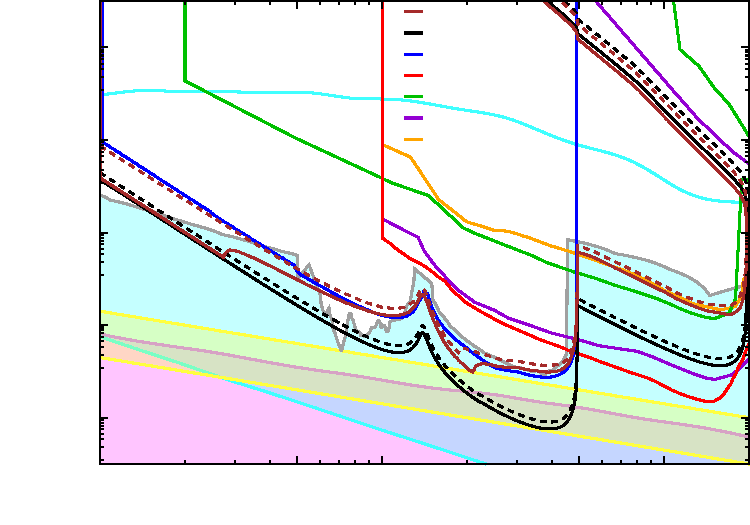
\includegraphics{pics/DUNE_HNL_E_real}}%
    \gplfronttext
  \end{picture}%
\endgroup
}}
			%\hspace{-0.5em}
			{\resizebox{0.5\linewidth}{!}{% GNUPLOT: LaTeX picture with Postscript
\begingroup
  \makeatletter
  \providecommand\color[2][]{%
    \GenericError{(gnuplot) \space\space\space\@spaces}{%
      Package color not loaded in conjunction with
      terminal option `colourtext'%
    }{See the gnuplot documentation for explanation.%
    }{Either use 'blacktext' in gnuplot or load the package
      color.sty in LaTeX.}%
    \renewcommand\color[2][]{}%
  }%
  \providecommand\includegraphics[2][]{%
    \GenericError{(gnuplot) \space\space\space\@spaces}{%
      Package graphicx or graphics not loaded%
    }{See the gnuplot documentation for explanation.%
    }{The gnuplot epslatex terminal needs graphicx.sty or graphics.sty.}%
    \renewcommand\includegraphics[2][]{}%
  }%
  \providecommand\rotatebox[2]{#2}%
  \@ifundefined{ifGPcolor}{%
    \newif\ifGPcolor
    \GPcolortrue
  }{}%
  \@ifundefined{ifGPblacktext}{%
    \newif\ifGPblacktext
    \GPblacktexttrue
  }{}%
  % define a \g@addto@macro without @ in the name:
  \let\gplgaddtomacro\g@addto@macro
  % define empty templates for all commands taking text:
  \gdef\gplbacktext{}%
  \gdef\gplfronttext{}%
  \makeatother
  \ifGPblacktext
    % no textcolor at all
    \def\colorrgb#1{}%
    \def\colorgray#1{}%
  \else
    % gray or color?
    \ifGPcolor
      \def\colorrgb#1{\color[rgb]{#1}}%
      \def\colorgray#1{\color[gray]{#1}}%
      \expandafter\def\csname LTw\endcsname{\color{white}}%
      \expandafter\def\csname LTb\endcsname{\color{black}}%
      \expandafter\def\csname LTa\endcsname{\color{black}}%
      \expandafter\def\csname LT0\endcsname{\color[rgb]{1,0,0}}%
      \expandafter\def\csname LT1\endcsname{\color[rgb]{0,1,0}}%
      \expandafter\def\csname LT2\endcsname{\color[rgb]{0,0,1}}%
      \expandafter\def\csname LT3\endcsname{\color[rgb]{1,0,1}}%
      \expandafter\def\csname LT4\endcsname{\color[rgb]{0,1,1}}%
      \expandafter\def\csname LT5\endcsname{\color[rgb]{1,1,0}}%
      \expandafter\def\csname LT6\endcsname{\color[rgb]{0,0,0}}%
      \expandafter\def\csname LT7\endcsname{\color[rgb]{1,0.3,0}}%
      \expandafter\def\csname LT8\endcsname{\color[rgb]{0.5,0.5,0.5}}%
    \else
      % gray
      \def\colorrgb#1{\color{black}}%
      \def\colorgray#1{\color[gray]{#1}}%
      \expandafter\def\csname LTw\endcsname{\color{white}}%
      \expandafter\def\csname LTb\endcsname{\color{black}}%
      \expandafter\def\csname LTa\endcsname{\color{black}}%
      \expandafter\def\csname LT0\endcsname{\color{black}}%
      \expandafter\def\csname LT1\endcsname{\color{black}}%
      \expandafter\def\csname LT2\endcsname{\color{black}}%
      \expandafter\def\csname LT3\endcsname{\color{black}}%
      \expandafter\def\csname LT4\endcsname{\color{black}}%
      \expandafter\def\csname LT5\endcsname{\color{black}}%
      \expandafter\def\csname LT6\endcsname{\color{black}}%
      \expandafter\def\csname LT7\endcsname{\color{black}}%
      \expandafter\def\csname LT8\endcsname{\color{black}}%
    \fi
  \fi
    \setlength{\unitlength}{0.0500bp}%
    \ifx\gptboxheight\undefined%
      \newlength{\gptboxheight}%
      \newlength{\gptboxwidth}%
      \newsavebox{\gptboxtext}%
    \fi%
    \setlength{\fboxrule}{0.5pt}%
    \setlength{\fboxsep}{1pt}%
\begin{picture}(7200.00,5040.00)%
    \gplgaddtomacro\gplbacktext{%
      \csname LTb\endcsname%%
      \put(849,1039){\makebox(0,0)[r]{\strut{}$10^{-10}$}}%
      \csname LTb\endcsname%%
      \put(849,1928){\makebox(0,0)[r]{\strut{}$10^{-8}$}}%
      \csname LTb\endcsname%%
      \put(849,2817){\makebox(0,0)[r]{\strut{}$10^{-6}$}}%
      \csname LTb\endcsname%%
      \put(849,3706){\makebox(0,0)[r]{\strut{}$10^{-4}$}}%
      \csname LTb\endcsname%%
      \put(849,4595){\makebox(0,0)[r]{\strut{}$10^{-2}$}}%
      \csname LTb\endcsname%%
      \put(2844,409){\makebox(0,0){\strut{}0.05}}%
      \csname LTb\endcsname%%
      \put(5552,409){\makebox(0,0){\strut{}0.5}}%
      \csname LTb\endcsname%%
      \put(7183,409){\makebox(0,0){\strut{}2}}%
      \csname LTb\endcsname%%
      \put(951,409){\makebox(0,0){\strut{}0.01}}%
      \csname LTb\endcsname%%
      \put(3659,409){\makebox(0,0){\strut{}0.1}}%
      \csname LTb\endcsname%%
      \put(6368,409){\makebox(0,0){\strut{}1}}%
    }%
    \gplgaddtomacro\gplfronttext{%
      \csname LTb\endcsname%%
      \put(153,2817){\rotatebox{-270}{\makebox(0,0){\strut{}$|U_{\mu N}|^2$}}}%
      \csname LTb\endcsname%%
      \put(4067,130){\makebox(0,0){\strut{}Mass $m_N$ (GeV)}}%
      \csname LTb\endcsname%%
      \put(4348,3713){\makebox(0,0)[l]{\strut{}FASER}}%
      \csname LTb\endcsname%%
      \put(4348,3917){\makebox(0,0)[l]{\strut{}MATHUSLA}}%
      \csname LTb\endcsname%%
      \put(4348,4121){\makebox(0,0)[l]{\strut{}NA62}}%
      \csname LTb\endcsname%%
      \put(4348,4325){\makebox(0,0)[l]{\strut{}SHiP}}%
      \csname LTb\endcsname%%
      \put(4348,4529){\makebox(0,0)[l]{\strut{}SBND}}%
      \csname LTb\endcsname%%
      \put(4348,4733){\makebox(0,0)[l]{\strut{}DUNE}}%
      \csname LTb\endcsname%%
      \put(4348,4937){\makebox(0,0)[l]{\strut{} }}%
      \csname LTb\endcsname%%
      \put(849,1039){\makebox(0,0)[r]{\strut{}$10^{-10}$}}%
      \csname LTb\endcsname%%
      \put(849,1928){\makebox(0,0)[r]{\strut{}$10^{-8}$}}%
      \csname LTb\endcsname%%
      \put(849,2817){\makebox(0,0)[r]{\strut{}$10^{-6}$}}%
      \csname LTb\endcsname%%
      \put(849,3706){\makebox(0,0)[r]{\strut{}$10^{-4}$}}%
      \csname LTb\endcsname%%
      \put(849,4595){\makebox(0,0)[r]{\strut{}$10^{-2}$}}%
      \csname LTb\endcsname%%
      \put(2844,409){\makebox(0,0){\strut{}0.05}}%
      \csname LTb\endcsname%%
      \put(5552,409){\makebox(0,0){\strut{}0.5}}%
      \csname LTb\endcsname%%
      \put(7183,409){\makebox(0,0){\strut{}2}}%
      \csname LTb\endcsname%%
      \put(951,409){\makebox(0,0){\strut{}0.01}}%
      \csname LTb\endcsname%%
      \put(3659,409){\makebox(0,0){\strut{}0.1}}%
      \csname LTb\endcsname%%
      \put(6368,409){\makebox(0,0){\strut{}1}}%
      \csname LTb\endcsname%%
      \put(4737,3261){\makebox(0,0){\strut{}\textbf{Excluded}}}%
      \csname LTb\endcsname%%
      \put(1766,996){\makebox(0,0){\strut{}\textbf{Weyl state}}}%
      \csname LTb\endcsname%%
      \put(2582,2239){\makebox(0,0){\strut{}\textbf{\shortstack{Pseudo-Dirac\\pair}}}}%
      \csname LTb\endcsname%%
      \put(2844,1484){\rotatebox{-5}{\makebox(0,0){\strut{}\textbf{Type I}}}}%
    }%
    \gplbacktext
    \put(0,0){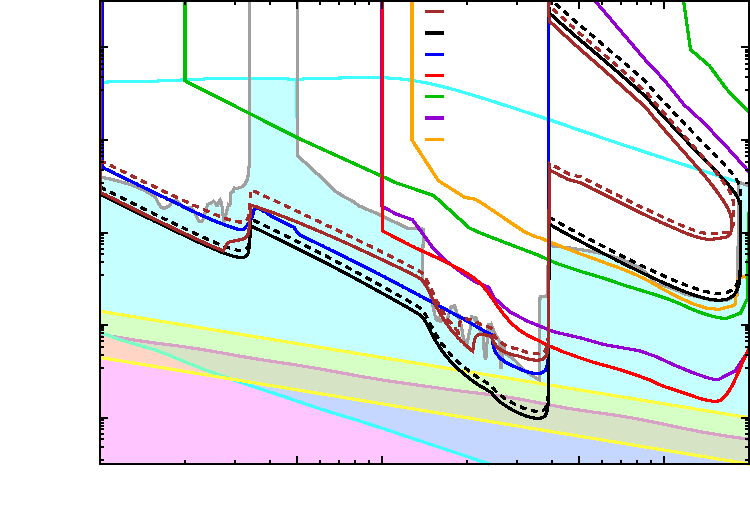
\includegraphics{pics/DUNE_HNL_M_real}}%
    \gplfronttext
  \end{picture}%
\endgroup
}}
		\end{minipage}
	}

	\vspace{0.5em}
	{\resizebox{0.5\linewidth}{!}{% GNUPLOT: LaTeX picture with Postscript
\begingroup
  \makeatletter
  \providecommand\color[2][]{%
    \GenericError{(gnuplot) \space\space\space\@spaces}{%
      Package color not loaded in conjunction with
      terminal option `colourtext'%
    }{See the gnuplot documentation for explanation.%
    }{Either use 'blacktext' in gnuplot or load the package
      color.sty in LaTeX.}%
    \renewcommand\color[2][]{}%
  }%
  \providecommand\includegraphics[2][]{%
    \GenericError{(gnuplot) \space\space\space\@spaces}{%
      Package graphicx or graphics not loaded%
    }{See the gnuplot documentation for explanation.%
    }{The gnuplot epslatex terminal needs graphicx.sty or graphics.sty.}%
    \renewcommand\includegraphics[2][]{}%
  }%
  \providecommand\rotatebox[2]{#2}%
  \@ifundefined{ifGPcolor}{%
    \newif\ifGPcolor
    \GPcolortrue
  }{}%
  \@ifundefined{ifGPblacktext}{%
    \newif\ifGPblacktext
    \GPblacktexttrue
  }{}%
  % define a \g@addto@macro without @ in the name:
  \let\gplgaddtomacro\g@addto@macro
  % define empty templates for all commands taking text:
  \gdef\gplbacktext{}%
  \gdef\gplfronttext{}%
  \makeatother
  \ifGPblacktext
    % no textcolor at all
    \def\colorrgb#1{}%
    \def\colorgray#1{}%
  \else
    % gray or color?
    \ifGPcolor
      \def\colorrgb#1{\color[rgb]{#1}}%
      \def\colorgray#1{\color[gray]{#1}}%
      \expandafter\def\csname LTw\endcsname{\color{white}}%
      \expandafter\def\csname LTb\endcsname{\color{black}}%
      \expandafter\def\csname LTa\endcsname{\color{black}}%
      \expandafter\def\csname LT0\endcsname{\color[rgb]{1,0,0}}%
      \expandafter\def\csname LT1\endcsname{\color[rgb]{0,1,0}}%
      \expandafter\def\csname LT2\endcsname{\color[rgb]{0,0,1}}%
      \expandafter\def\csname LT3\endcsname{\color[rgb]{1,0,1}}%
      \expandafter\def\csname LT4\endcsname{\color[rgb]{0,1,1}}%
      \expandafter\def\csname LT5\endcsname{\color[rgb]{1,1,0}}%
      \expandafter\def\csname LT6\endcsname{\color[rgb]{0,0,0}}%
      \expandafter\def\csname LT7\endcsname{\color[rgb]{1,0.3,0}}%
      \expandafter\def\csname LT8\endcsname{\color[rgb]{0.5,0.5,0.5}}%
    \else
      % gray
      \def\colorrgb#1{\color{black}}%
      \def\colorgray#1{\color[gray]{#1}}%
      \expandafter\def\csname LTw\endcsname{\color{white}}%
      \expandafter\def\csname LTb\endcsname{\color{black}}%
      \expandafter\def\csname LTa\endcsname{\color{black}}%
      \expandafter\def\csname LT0\endcsname{\color{black}}%
      \expandafter\def\csname LT1\endcsname{\color{black}}%
      \expandafter\def\csname LT2\endcsname{\color{black}}%
      \expandafter\def\csname LT3\endcsname{\color{black}}%
      \expandafter\def\csname LT4\endcsname{\color{black}}%
      \expandafter\def\csname LT5\endcsname{\color{black}}%
      \expandafter\def\csname LT6\endcsname{\color{black}}%
      \expandafter\def\csname LT7\endcsname{\color{black}}%
      \expandafter\def\csname LT8\endcsname{\color{black}}%
    \fi
  \fi
    \setlength{\unitlength}{0.0500bp}%
    \ifx\gptboxheight\undefined%
      \newlength{\gptboxheight}%
      \newlength{\gptboxwidth}%
      \newsavebox{\gptboxtext}%
    \fi%
    \setlength{\fboxrule}{0.5pt}%
    \setlength{\fboxsep}{1pt}%
\begin{picture}(7200.00,5040.00)%
    \gplgaddtomacro\gplbacktext{%
      \csname LTb\endcsname%%
      \put(849,595){\makebox(0,0)[r]{\strut{}$10^{-10}$}}%
      \csname LTb\endcsname%%
      \put(849,1484){\makebox(0,0)[r]{\strut{}$10^{-8}$}}%
      \csname LTb\endcsname%%
      \put(849,2373){\makebox(0,0)[r]{\strut{}$10^{-6}$}}%
      \csname LTb\endcsname%%
      \put(849,3261){\makebox(0,0)[r]{\strut{}$10^{-4}$}}%
      \csname LTb\endcsname%%
      \put(849,4150){\makebox(0,0)[r]{\strut{}$10^{-2}$}}%
      \csname LTb\endcsname%%
      \put(849,5039){\makebox(0,0)[r]{\strut{}$10^{0}$}}%
      \csname LTb\endcsname%%
      \put(2844,409){\makebox(0,0){\strut{}0.05}}%
      \csname LTb\endcsname%%
      \put(5552,409){\makebox(0,0){\strut{}0.5}}%
      \csname LTb\endcsname%%
      \put(7183,409){\makebox(0,0){\strut{}2}}%
      \csname LTb\endcsname%%
      \put(951,409){\makebox(0,0){\strut{}0.01}}%
      \csname LTb\endcsname%%
      \put(3659,409){\makebox(0,0){\strut{}0.1}}%
      \csname LTb\endcsname%%
      \put(6368,409){\makebox(0,0){\strut{}1}}%
    }%
    \gplgaddtomacro\gplfronttext{%
      \csname LTb\endcsname%%
      \put(153,2817){\rotatebox{-270}{\makebox(0,0){\strut{}$|U_{\tau N}|^2$}}}%
      \csname LTb\endcsname%%
      \put(4067,130){\makebox(0,0){\strut{}Mass (GeV)}}%
      \csname LTb\endcsname%%
      \put(1808,2584){\makebox(0,0)[l]{\strut{}FASER}}%
      \csname LTb\endcsname%%
      \put(1808,2788){\makebox(0,0)[l]{\strut{}MATHUSLA}}%
      \csname LTb\endcsname%%
      \put(1808,2992){\makebox(0,0)[l]{\strut{}NA62}}%
      \csname LTb\endcsname%%
      \put(1808,3196){\makebox(0,0)[l]{\strut{}SHiP}}%
      \csname LTb\endcsname%%
      \put(1808,3400){\makebox(0,0)[l]{\strut{}DUNE}}%
      \csname LTb\endcsname%%
      \put(1808,3604){\makebox(0,0)[l]{\strut{} }}%
      \csname LTb\endcsname%%
      \put(849,595){\makebox(0,0)[r]{\strut{}$10^{-10}$}}%
      \csname LTb\endcsname%%
      \put(849,1484){\makebox(0,0)[r]{\strut{}$10^{-8}$}}%
      \csname LTb\endcsname%%
      \put(849,2373){\makebox(0,0)[r]{\strut{}$10^{-6}$}}%
      \csname LTb\endcsname%%
      \put(849,3261){\makebox(0,0)[r]{\strut{}$10^{-4}$}}%
      \csname LTb\endcsname%%
      \put(849,4150){\makebox(0,0)[r]{\strut{}$10^{-2}$}}%
      \csname LTb\endcsname%%
      \put(849,5039){\makebox(0,0)[r]{\strut{}$10^{0}$}}%
      \csname LTb\endcsname%%
      \put(2844,409){\makebox(0,0){\strut{}0.05}}%
      \csname LTb\endcsname%%
      \put(5552,409){\makebox(0,0){\strut{}0.5}}%
      \csname LTb\endcsname%%
      \put(7183,409){\makebox(0,0){\strut{}2}}%
      \csname LTb\endcsname%%
      \put(951,409){\makebox(0,0){\strut{}0.01}}%
      \csname LTb\endcsname%%
      \put(3659,409){\makebox(0,0){\strut{}0.1}}%
      \csname LTb\endcsname%%
      \put(6368,409){\makebox(0,0){\strut{}1}}%
      \csname LTb\endcsname%%
      \put(2844,4595){\makebox(0,0){\strut{}\textbf{Excluded}}}%
      \csname LTb\endcsname%%
      \put(1766,906){\makebox(0,0){\strut{}\textbf{Weyl state}}}%
      \csname LTb\endcsname%%
      \put(2844,1928){\makebox(0,0){\strut{}\textbf{\shortstack{Pseudo-Dirac\\pair}}}}%
      \csname LTb\endcsname%%
      \put(2844,1039){\rotatebox{-5}{\makebox(0,0){\strut{}\textbf{Type I}}}}%
    }%
    \gplbacktext
    \put(0,0){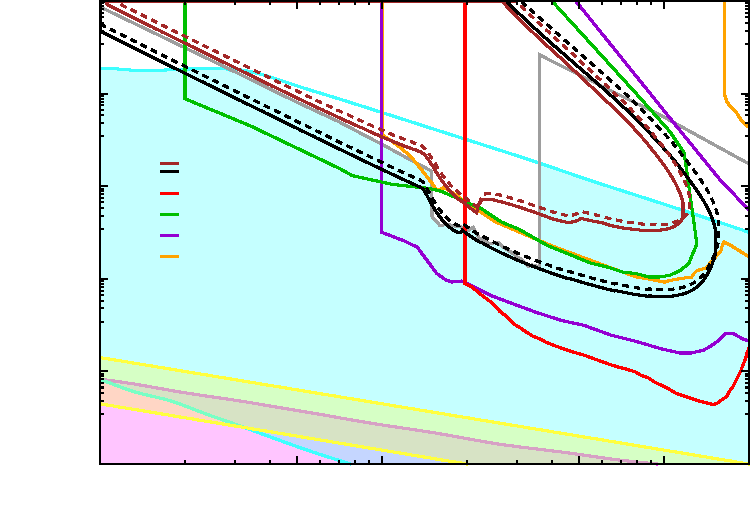
\includegraphics{pics/DUNE_HNL_T_real}}%
    \gplfronttext
  \end{picture}%
\endgroup
}}
	%
	\vspace{-0.2em}
	\caption{The 90\,\% C.L. sensitivity regions for dominant mixings %
		$|U_{e N}|^2$ (top left), $|U_{\mu N}|^2$ (top right), and $|U_{\tau N}|^2$ (bottom) are presented %
		combining results for channels with good discovery prospects (see text).
		The study is performed for Majorana neutrinos (solid) and Dirac neutrinos (dashed), %
		in the case of no background (black) and after the background analysis (brown).
		The region excluded by experimental constraints (grey) is obtained by combining the results from
		PS191~\cite{Bernardi:1985ny, Bernardi:1987ek}, %
		peak searches~\cite{Artamonov:2014urb, Britton:1992pg, Britton:1992xv, Aguilar-Arevalo:2017vlf, Aguilar-Arevalo:2019owf}, %
		CHARM~\cite{Vilain:1994vg}, NuTeV~\cite{Vaitaitis:1999wq}, DELPHI~\cite{Abreu:1996pa}, and T2K~\cite{Abe:2019kgx}.
		The sensitivity for DUNE ND (black) is compared to the predictions of future experiments, %
		SBN~\cite{Ballett:2016opr} (blue), %
		SHiP~\cite{Alekhin:2015byh} (red), NA62~\cite{Drewes:2018irr} (green), MATHUSLA~\cite{Curtin:2018mvb} (purple), %
		and FASER~\cite{Kling:2018wct} with 1\,m radius (orange).
		The shaded areas corresponds to possible neutrino mass models considered in this article: %
		the simulations of the ISS\,(2,2) and ISS\,(2,3) models where the lightest %
		pseudo-Dirac pair is the neutrino decaying in the ND (cyan); %
		the ISS\,(2,3) scenario when the single Majorana state is responsible for a signal (magenta); %
		the type~I seesaw scenario with a neutrino mass starting from \np{20}\,meV to \np{0.2}\,eV (yellow).}
	\label{fig:sensAll}
\end{figure}

To appreciate the ND performance, we make a comparison with results of previous experiments, %
in particular PS191~\cite{Bernardi:1985ny, Bernardi:1987ek}, peak searches~\cite{Artamonov:2014urb, Britton:1992pg, Britton:1992xv}, %
CHARM~\cite{Vilain:1994vg}, NuTeV~\cite{Vaitaitis:1999wq}, DELPHI~\cite{Abreu:1996pa}, and T2K~\cite{Abe:2019kgx}.
We find that the DUNE ND can increase the bound on the electronic and muonic mixing elements %
for masses $m_N < m_{K^0}$ with respect to past experiments.
The constraint on the tauonic mixing is at least comparable with previous measurements.
For masses above, for which neutrino production relies on charm meson decays, the existing bounds %
are improved for the electronic mixing and the tauonic mixing, while a conservative result %
can be achieved in the muonic case.
We also overlay the prospects for the SBN programme~\cite{Ballett:2016opr}, %
NA62~\cite{Drewes:2018irr}, and the proposed SHiP~\cite{Alekhin:2015byh}, MATHUSLA~\cite{Curtin:2018mvb}, %
and FASER~\cite{Kling:2018wct} with 1\,m radius.
DUNE ND will give the best sensitivity for masses below the 0.5\,GeV in all channels, but the tauonic one.
However, anywhere the $D_s$ meson production is involved, the experiment cannot outperform the predicted %
sensitivity of the SHiP experiment which will deploy a 400\,GeV proton beam on a titanium-zinc-molybdenum alloy %
target, enhancing the production of charm and bottom mesons.
MATHUSLA will have a similar sensitivity, collecting particles from the High Luminosity LHC phase.
NA62 gives better results for the $|U_{\mu N}|^2$ mixing, but DUNE has a better sensitivity %
to the electron and tau channels.
FASER is comparable to NA62 in sensitivity, but it can reach regions of the parameter space beyond the 2\,GeV limit %
to which DUNE is not sensitive.
Comparing to previous similar studies, the sensitivities estimated in this analysis give stronger %
or at least comparable bounds than the ones in \refref{Krasnov:2019kdc}, 
where a different ND configuration is assumed, and no background study was performed.
More specifically, the limits on $|U_{eN}|^2$ are stronger, even considering the background events.
This is true also for the limits on $|U_{\mu N}|^2$, but only for masses below 500 MeV: %
in \refref{Krasnov:2019kdc} the sensitivity to masses above this threshold is enhanced by the contribution %
from B meson, which is not estimated in this study.
For the same reason, the limits on $|U_{\tau N}|^2$ prove to be comparable to our result, %
despite accounting only for the $D_s$ meson component.

We then compare the overall sensitivity to regions allowed by neutrino mass models.
In the electronic and muonic channels, DUNE ND will be sensitive to a large part of the pseudo-Dirac regions, %
corresponding to ISS\,(2,2) and ISS\,(2,3) models, %
part of which have been already excluded by past experiments.
DUNE will close the gap and put to test type I seesaw parameters, especially for HNL masses between 0.2 and 0.5\,GeV, %
starting to reach the region of ISS\,(2,3) with large lepton number violation.
For the tauonic channel, the experiment will probe only a small portion %
of pseudo-Dirac pairs from ISS\,(2,2) and ISS\,(2,3) models.
The sensitivity is not high enough to reach type I and Majorana state regions, which not even the dedicated experiment SHiP can.

\begin{figure}
	\centering
	{\resizebox{\linewidth}{!}{% GNUPLOT: LaTeX picture with Postscript
\begingroup
  \makeatletter
  \providecommand\color[2][]{%
    \GenericError{(gnuplot) \space\space\space\@spaces}{%
      Package color not loaded in conjunction with
      terminal option `colourtext'%
    }{See the gnuplot documentation for explanation.%
    }{Either use 'blacktext' in gnuplot or load the package
      color.sty in LaTeX.}%
    \renewcommand\color[2][]{}%
  }%
  \providecommand\includegraphics[2][]{%
    \GenericError{(gnuplot) \space\space\space\@spaces}{%
      Package graphicx or graphics not loaded%
    }{See the gnuplot documentation for explanation.%
    }{The gnuplot epslatex terminal needs graphicx.sty or graphics.sty.}%
    \renewcommand\includegraphics[2][]{}%
  }%
  \providecommand\rotatebox[2]{#2}%
  \@ifundefined{ifGPcolor}{%
    \newif\ifGPcolor
    \GPcolortrue
  }{}%
  \@ifundefined{ifGPblacktext}{%
    \newif\ifGPblacktext
    \GPblacktexttrue
  }{}%
  % define a \g@addto@macro without @ in the name:
  \let\gplgaddtomacro\g@addto@macro
  % define empty templates for all commands taking text:
  \gdef\gplbacktext{}%
  \gdef\gplfronttext{}%
  \makeatother
  \ifGPblacktext
    % no textcolor at all
    \def\colorrgb#1{}%
    \def\colorgray#1{}%
  \else
    % gray or color?
    \ifGPcolor
      \def\colorrgb#1{\color[rgb]{#1}}%
      \def\colorgray#1{\color[gray]{#1}}%
      \expandafter\def\csname LTw\endcsname{\color{white}}%
      \expandafter\def\csname LTb\endcsname{\color{black}}%
      \expandafter\def\csname LTa\endcsname{\color{black}}%
      \expandafter\def\csname LT0\endcsname{\color[rgb]{1,0,0}}%
      \expandafter\def\csname LT1\endcsname{\color[rgb]{0,1,0}}%
      \expandafter\def\csname LT2\endcsname{\color[rgb]{0,0,1}}%
      \expandafter\def\csname LT3\endcsname{\color[rgb]{1,0,1}}%
      \expandafter\def\csname LT4\endcsname{\color[rgb]{0,1,1}}%
      \expandafter\def\csname LT5\endcsname{\color[rgb]{1,1,0}}%
      \expandafter\def\csname LT6\endcsname{\color[rgb]{0,0,0}}%
      \expandafter\def\csname LT7\endcsname{\color[rgb]{1,0.3,0}}%
      \expandafter\def\csname LT8\endcsname{\color[rgb]{0.5,0.5,0.5}}%
    \else
      % gray
      \def\colorrgb#1{\color{black}}%
      \def\colorgray#1{\color[gray]{#1}}%
      \expandafter\def\csname LTw\endcsname{\color{white}}%
      \expandafter\def\csname LTb\endcsname{\color{black}}%
      \expandafter\def\csname LTa\endcsname{\color{black}}%
      \expandafter\def\csname LT0\endcsname{\color{black}}%
      \expandafter\def\csname LT1\endcsname{\color{black}}%
      \expandafter\def\csname LT2\endcsname{\color{black}}%
      \expandafter\def\csname LT3\endcsname{\color{black}}%
      \expandafter\def\csname LT4\endcsname{\color{black}}%
      \expandafter\def\csname LT5\endcsname{\color{black}}%
      \expandafter\def\csname LT6\endcsname{\color{black}}%
      \expandafter\def\csname LT7\endcsname{\color{black}}%
      \expandafter\def\csname LT8\endcsname{\color{black}}%
    \fi
  \fi
    \setlength{\unitlength}{0.0500bp}%
    \ifx\gptboxheight\undefined%
      \newlength{\gptboxheight}%
      \newlength{\gptboxwidth}%
      \newsavebox{\gptboxtext}%
    \fi%
    \setlength{\fboxrule}{0.5pt}%
    \setlength{\fboxsep}{1pt}%
\begin{picture}(14400.00,5040.00)%
    \gplgaddtomacro\gplbacktext{%
      \csname LTb\endcsname%%
      \put(444,972){\makebox(0,0)[r]{\strut{}\np{e-1}}}%
      \put(444,2740){\makebox(0,0)[r]{\strut{}\np{e0}}}%
      \put(444,4507){\makebox(0,0)[r]{\strut{}\np{e1}}}%
      \put(576,220){\makebox(0,0){\strut{}\np{e-10}}}%
      \put(1497,220){\makebox(0,0){\strut{}\np{e-8}}}%
      \put(2419,220){\makebox(0,0){\strut{}\np{e-6}}}%
      \put(3340,220){\makebox(0,0){\strut{}\np{e-4}}}%
      \put(4262,220){\makebox(0,0){\strut{}\np{e-2}}}%
    }%
    \gplgaddtomacro\gplfronttext{%
      \csname LTb\endcsname%%
      \put(-304,2739){\rotatebox{-270}{\makebox(0,0){\strut{}$\Delta m_{4 1}^2 $}}}%
      \put(2879,-110){\makebox(0,0){\strut{}$|U_{e 4}|^2$}}%
      \csname LTb\endcsname%%
      \put(1167,4844){\makebox(0,0)[l]{\strut{}DANSS}}%
      \csname LTb\endcsname%%
      \put(1167,4580){\makebox(0,0)[l]{\strut{}NEOS}}%
      \csname LTb\endcsname%%
      \put(1167,4316){\makebox(0,0)[l]{\strut{}STEREO}}%
      \csname LTb\endcsname%%
      \put(1167,4052){\makebox(0,0)[l]{\strut{}SK + IC}}%
    }%
    \gplgaddtomacro\gplbacktext{%
      \csname LTb\endcsname%%
      \put(5052,972){\makebox(0,0)[r]{\strut{}}}%
      \put(5052,2740){\makebox(0,0)[r]{\strut{}}}%
      \put(5052,4507){\makebox(0,0)[r]{\strut{}}}%
      \put(5184,220){\makebox(0,0){\strut{}\np{e-12}}}%
      \put(5952,220){\makebox(0,0){\strut{}\np{e-10}}}%
      \put(6720,220){\makebox(0,0){\strut{}\np{e-8}}}%
      \put(7488,220){\makebox(0,0){\strut{}\np{e-6}}}%
      \put(8255,220){\makebox(0,0){\strut{}\np{e-4}}}%
      \put(9023,220){\makebox(0,0){\strut{}\np{e-2}}}%
    }%
    \gplgaddtomacro\gplfronttext{%
      \csname LTb\endcsname%%
      \put(7487,-110){\makebox(0,0){\strut{}$4 |U_{e 4}|^2 |U_{\mu 4}|^2$}}%
      \csname LTb\endcsname%%
      \put(5775,4844){\makebox(0,0)[l]{\strut{}MiniBooNE}}%
      \csname LTb\endcsname%%
      \put(5775,4580){\makebox(0,0)[l]{\strut{}KARMEN}}%
      \csname LTb\endcsname%%
      \put(5775,4316){\makebox(0,0)[l]{\strut{}OPERA}}%
    }%
    \gplgaddtomacro\gplbacktext{%
      \csname LTb\endcsname%%
      \put(9660,972){\makebox(0,0)[r]{\strut{}}}%
      \put(9660,2740){\makebox(0,0)[r]{\strut{}}}%
      \put(9660,4507){\makebox(0,0)[r]{\strut{}}}%
      \put(14399,220){\makebox(0,0){\strut{}\np{e0}}}%
      \put(9792,220){\makebox(0,0){\strut{}\np{e-10}}}%
      \put(10713,220){\makebox(0,0){\strut{}\np{e-8}}}%
      \put(11635,220){\makebox(0,0){\strut{}\np{e-6}}}%
      \put(12556,220){\makebox(0,0){\strut{}\np{e-4}}}%
      \put(13478,220){\makebox(0,0){\strut{}\np{e-2}}}%
    }%
    \gplgaddtomacro\gplfronttext{%
      \csname LTb\endcsname%%
      \put(12095,-110){\makebox(0,0){\strut{}$|U_{\mu 4}|^2$}}%
      \csname LTb\endcsname%%
      \put(10383,4844){\makebox(0,0)[l]{\strut{}$\nu_\mu\to\nu_\mu$}}%
    }%
    \gplbacktext
    \put(0,0){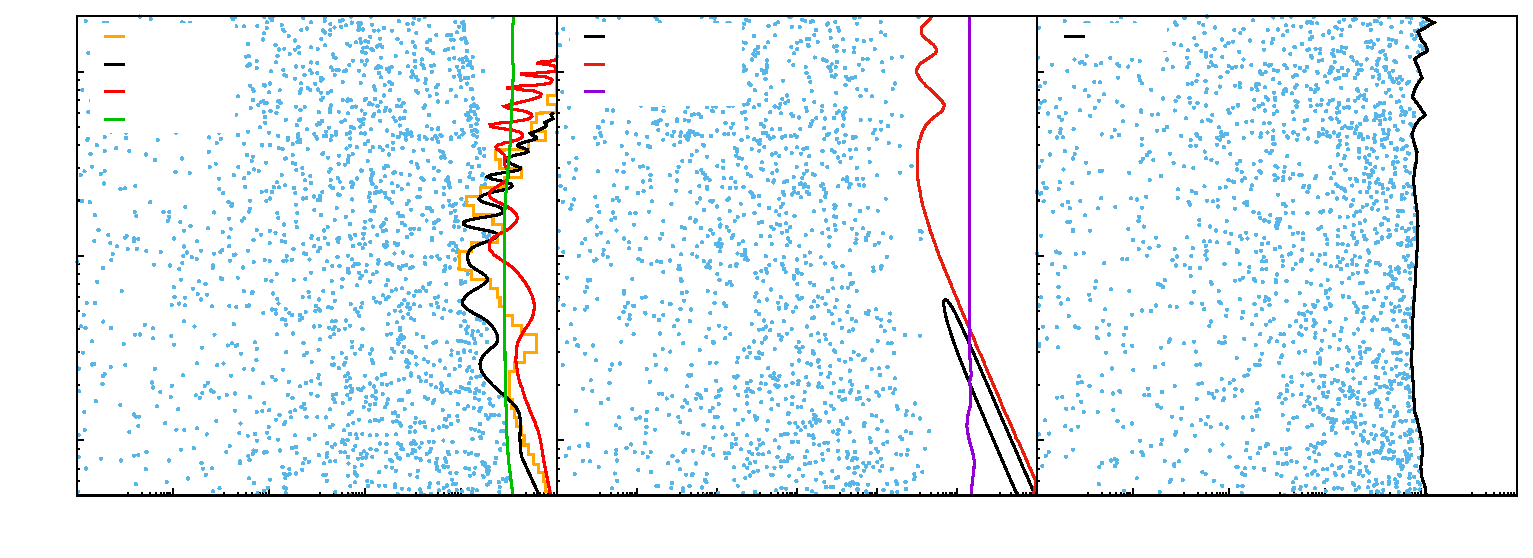
\includegraphics{pics/multiSBL}}%
    \gplfronttext
  \end{picture}%
\endgroup
}}
	%{\resizebox{0.5\linewidth}{!}{\input{pics/oscUe.tex}}}
	%\hspace{-1em}
	%{\resizebox{0.5\linewidth}{!}{\input{pics/oscUem.tex}}}
	%\hspace{-1em}
	%{\resizebox{0.5\linewidth}{!}{\input{pics/oscUm.tex}}}
	%
	\caption{One of the two ISS\,(2,3) realisations considered presents a Majorana state at masses comparable with SBL experiments.
		We show the results of the ISS\,(2,3) simulation (blue dots) for $\Delta m_{4 1}^2$ against combination of mixing angles and %
		the experimental result at 90\,\% C.L.: %
		$|U_{e 4}|^2$~(left) compared to Super-Kamiokande and IceCube combined~\cite{Dentler:2018sju} and DANSS~\cite{Alekseev:2018efk}, %
		\mbox{$\sin^2 2\theta{_\mu e} = 4|U_{e 4}|^2|U_{\mu 4}|^2$} (middle) compared to KARMEN2, OPERA and MiniBooNE~\cite{Aguilar-Arevalo:2018gpe},
		and $|U_{\mu 4}|^2$ (right) compared to a combined $\nu_\mu$ disappearance analysis~\cite{Dentler:2018sju}.
		Only the points generated by matrices which pass the experimental constraints are shown here.}
	\label{fig:sblosc}
\end{figure}

The ISS\,(2,3) scenario in which the pseudo-Dirac pair is accessible by the experiment also predicts a light %
Majorana state, the mass of which is controlled by the small LNV perturbations.
This entails the presence of a third mass splitting $\Delta m^2_{4 1}$, which could give %
an active-sterile oscillation signature in short baseline experiments.
In figure Fig.~\ref{fig:sblosc}, the new mass splitting is plotted against the mixings $|U_{e 4}|^2$, %
$|U_{\mu 4}|^2$ and the combination usually referred to as %
$\sin^2 2\theta_{\mu e} \equiv 4 |U_{e 4}|^2|U_{\mu 4}|^2$.
The mass splittings generated in the matrix scan span from %
$\Delta m^2_{3 1} \simeq \np{0.0025}$\,eV\tapi{2} up to \np{e4}\,eV\tapi{2}, and the squared mixings cover a large region, %
down to \np{e-14} for all the flavours.
The reactor anomalies could be soon excluded at the 90\,\% C.L. by the DANSS experiment~\cite{Alekseev:2018efk} %
and the allowed regions from LSND~\cite{Aguilar:2001ty} and %
MiniBooNE~\cite{Aguilar-Arevalo:2012fmn, Aguilar-Arevalo:2013pmq, Aguilar-Arevalo:2018gpe} %
require values of $\sin^2 2\theta_{\mu e} \gtrsim \np{e-3}$.
Given the results of the matrix scan, it is unlikely that one of the ISS\,(2,3) realisations %
considered in this work could link an heavy neutrino--like signal in DUNE ND and explain a short baseline anomaly at the same time, %
\enlargethispage{\baselineskip}
unless for sparse and very fine-tuned points.
